\noindent Unter einer Hypothese wird in der Statistik eine Annahme \"{u}ber einen Sachverhalt verstanden, der \"{u}ber die Verteilung einer Zufallsvariable beschrieben werden kann. Der Test einer Hypothese ist ein Pr\"{u}fverfahren, das angewendet wird, um die Hypothese anzunehmen oder zu verwerfen. Hypothesentests sind damit Grundlage f\"{u}r Entscheidungen, die Theorie der Hypothesentests wird deshalb auch als Theorie der Entscheidungen bezeichnet.\newline

\noindent \"{A}hnlich wie bei der Bestimmung von Konfidenzbereichen wird auch beim Testen von Hypothesen von der Stichprobe auf die Grundgesamtheit geschlossen. Deshalb gibt es beim Hypothesentest keine vollkommen sicheren Schl\"{u}sse, eine Hypothese wird immer in Kombination mit einem definierten Fehlerrisiko getestet. Ein Hypothesentest sagt aus, ob auf Basis der vorliegenden Stichprobe eine Hypothese aufrechterhalten werden kann oder verworfen werden muss. \newline

\noindent In der Praxis kann meist zumindest n\"{a}herungsweise von einer normalverteilten Grundgesamtheit ausgegangen werden. Deshalb wird bei der folgenden Diskussion von Hypothesentests von normalverteilten Grundgesamtheiten ausgegangen. 


\subsection{Motivation mit einem einf\"{u}hrenden Beispiel}

\noindent Zur Kontrolle von Fertigungsprozessen werden an vielen Stellen Prozesskontrollen durchgef\"{u}hrt. Dadurch soll sichergestellt werden, dass die einzelnen Fertigungsschritte gem\"{a}{\ss} ihrer Spezifikation arbeiten. Signifikante Abweichungen von diesem Soll-Zustand werden durch die Prozesskontrolle erkannt und anschlie{\ss}end beseitigt. Als Beispiel wird das Gewicht einer Kleberaupe betrachtet. Zur Prozesskontrolle wird eine Stichprobe von N = 5 Teilen ausgew\"{a}hlt und das Gewicht der Kleberaupe vermessen. Das Gewicht aller gefertigten Teile soll als Mittelwert µ das spezifizierte Klebergewicht µ$_{0}$ aufweisen. Falls das Gewicht signifikant abweicht, muss bei den Maschineneinstellungen die Sollmenge korrigiert werden. Eine signifikante Abweichung soll auf Basis des Stichprobenmittelwertes $\overline{\mathrm{x}}$ erkannt werden. Die Standardabweichung $\sigma$ f\"{u}r den Prozess ergibt sich aus der Fertigungseinrichtung, sie wird in diesem Kapitel als bekannt vorausgesetzt. \newline

\noindent Die Aufgabe kann mit einem Hypothesentest gel\"{o}st werden, der mit den folgenden Hypothesen arbeitet:

\begin{itemize}
    \item Nullhypothese H$_{0}$: Mittelwert stimmt mit dem spezifizierten Wert \"{u}berein, µ = µ$_{0}$
    \item Alternativhypothese H$_{1}$: Mittelwert weicht signifikant von dem spezifizierten Wert ab, µ $\neq$ µ$_{0}$
\end{itemize}

\noindent Eine starke Abweichung des Stichprobenmittelwertes $\overline{\mathrm{x}}$ von dem spezifizierten Sollwert µ$_{0}$ w\"{u}rde signalisieren, dass der Fertigungsprozess \"{u}berpr\"{u}ft werden muss. Zur Bestimmung des Grenzwertes, bei dem die Hypothese gerade eben noch akzeptiert wird, wird davon ausgegangen, dass die Null-Hypothese H$_{0}$ gilt. In dem Fall weist der Stichprobenmittelwert eine Normalverteilung mit dem Mittelwert µ$_{0}$ und der Varianz $\sigma^{2}$/N auf. Die Verteilung ist in Bild \ref{fig:DiagnoseFeuchtesensor1} dargestellt.

\clearpage

\noindent 
\begin{figure}[H]
  \centerline{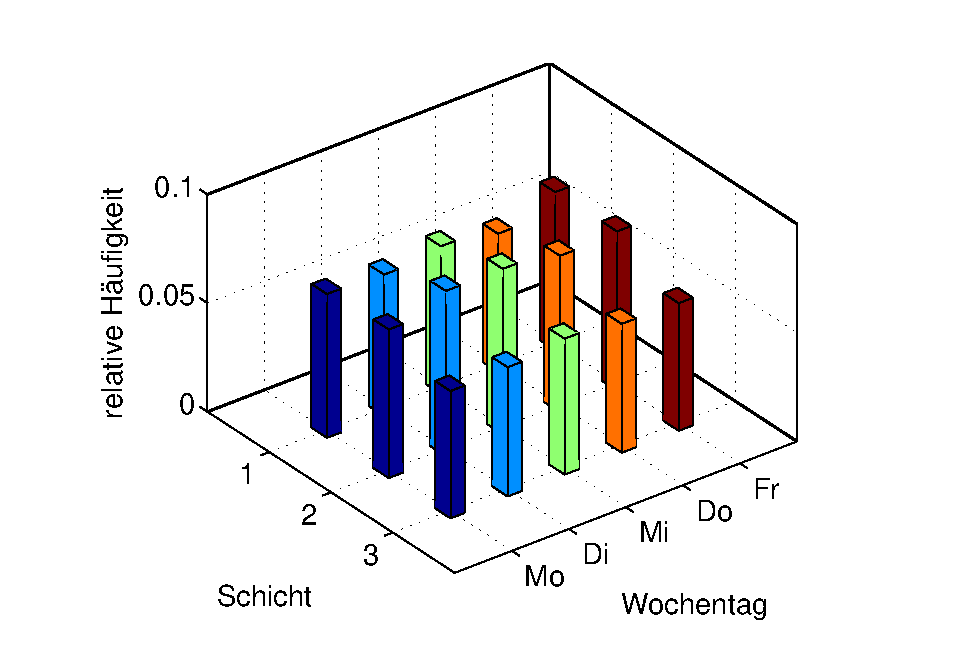
\includegraphics[width=0.5\textwidth]{Kapitel6/Bilder/image1}}
  \caption{Darstellung des Hypothesentests in der Wahrscheinlichkeitsdichte der Normalverteilung, die blauen Fl\"{a}chen entsprechen der Wahrscheinlichkeit P($\overline{\mathrm{x}}\mathrm{<}{\overline{\mathrm{x}}}_1$) und P($\overline{\mathrm{x}} \mathrm{>}{\overline{\mathrm{x}}}_2$)}
  \label{fig:DiagnoseFeuchtesensor1}
\end{figure}

\noindent Damit ein \"{u}ber die Stichprobe gesch\"{a}tzter Mittelwert $\overline{\mathrm{x}}$ mit einer spezifizierten Wahrscheinlichkeit zu der Normalverteilung mit dem Mittelwert µ$_{0}$ und der Varianz $\sigma^{2}$/N geh\"{o}rt, muss dieser in dem Intervall ${\overline{\mathrm{x}}}_1$ $\mathrm{<}$ $\overline{\mathrm{x}}$ $\leq$ ${\overline{\mathrm{x}}}_2$ liegen. Wird die Wahrscheinlichkeit daf\"{u}r mit $\gamma$ bezeichnet, gilt die Gleichung

\begin{equation}\label{eq:sixone}
P\left(\bar{x}_{1} <\bar{x}\le \bar{x}_{2} \right)=\gamma
\end{equation}

\noindent Das Intervall mit den Grenzen ${\overline{\mathrm{x}}}_1$ und ${\overline{\mathrm{x}}}_2$ wird als Annahmebereich f\"{u}r die Hypothese H${}_{0}$ bezeichnet. Liegt ein gesch\"{a}tzter Mittelwert $\overline{\mathrm{x}}$ au{\ss}erhalb des Intervalls ${\overline{\mathrm{x}}}_1$ $\mathrm{<}$ $\overline{\mathrm{x}}$ $\leq$ ${\overline{\mathrm{x}}}_2$, wird die Hypothese H${}_{0}$ verworfen, obwohl der gesch\"{a}tzte Mittelwert $\overline{\mathrm{x}}$ mit der Irrtumswahrscheinlichkeit

\begin{equation}\label{eq:sixtwo}
\alpha =1-\gamma
\end{equation}

\noindent zu der in Bild \ref{fig:DiagnoseFeuchtesensor1} dargestellten Verteilung geh\"{o}ren kann. Die Irrtumswahrscheinlichkeit wird auch als Signifikanzniveau $\alpha$ des statistischen Tests bezeichnet und zur Berechnung der Grenzen ${\overline{\mathrm{x}}}_1$ und ${\overline{\mathrm{x}}}_2$ herangezogen.\newline

\noindent Das Vorgehen zur Berechnung des Annahmebereiches entspricht weitgehend dem der Berechnung eines Konfidenzbereiches. Es beruht darauf, eine Zufallsvariable mit einer bekannten Verteilung zu finden, in deren Beschreibung die Hypothese H${}_{0}$ und der bekannte Parameter der Stichprobe vorkommen. F\"{u}r das Beispiel des Gewichts von Kleberaupen gilt dies f\"{u}r die standardnormalverteilte Zufallsvariable

\begin{equation}\label{eq:sixthree}
z=\dfrac{\bar{x}-\mu _{0}}{\sigma /\sqrt{N}}
\end{equation}

\noindent Mit dieser Verteilung wird nach Gleichung \eqref{eq:sixone} die Wahrscheinlichkeit $\gamma$, mit der die Variable z innerhalb des Intervalls c$_{1}$ {\dots} c$_{2}$ liegt, definiert als

\begin{equation}\label{eq:sixfour}
\gamma =P\left(c_{1} <z\le c_{2} \right)=F(c_{2})-F(c_{1})
\end{equation}

\noindent Bei Annahme eines symmetrischen Tests ergeben sich die Konstanten c$_{1}$ und c$_{2}$ aus den Bedingungen

\begin{equation}\label{eq:sixfive}
F(c_{1})=\dfrac{1-\gamma}{2} =\dfrac{\alpha}{2}
\end{equation}

\noindent und

\begin{equation}\label{eq:sixsix}
F(c_{2})=1-\dfrac{1-\gamma}{2} =1-\dfrac{\alpha}{2}
\end{equation}

\noindent Aufl\"{o}sen nach c$_{1}$ und c$_{2}$ f\"{u}hrt zu

\begin{equation}\label{eq:sixseven}
c_{1} =F^{-1} \left(\dfrac{\alpha }{2} \right)
\end{equation}

\noindent und

\begin{equation}\label{eq:sixeight}
c_{2} =F^{-1} \left(1-\dfrac{\alpha }{2} \right)
\end{equation}

\noindent Durch Umformungen von Gleichung \eqref{eq:sixfour} ergibt sich ein Ausdruck f\"{u}r den Annahmebereich der Nullhypothese, n\"{a}mlich dass der gesch\"{a}tzte Mittelwert $\overline{\mathrm{x}}$, mit einer spezifizierten Wahrscheinlichkeit $\gamma$, zu der Normalverteilung mit dem Mittelwert µ$_{0}$ und der Varianz $\sigma^{2}$/N geh\"{o}rt.

\begin{equation}\label{eq:sixnine}
\gamma =P\left(c_{1} <\dfrac{\bar{x}-\mu _{0} }{\sigma /\sqrt{N}} \le c_{2} \right)=P\left(\mu _{0} +\dfrac{c_{1} \cdot \sigma }{\sqrt{N}} <\bar{x}\le \mu _{0} +\dfrac{c_{2} \cdot \sigma }{\sqrt{N}} \right)
\end{equation}

\noindent F\"{u}r das Beispiel Prozesskontrolle von Kleberaupen soll der Annahmebereich daf\"{u}r berechnet werden, dass der Mittelwert aus einer Stichprobe mit N = 5 Teilen dem spezifizierten Mittelwert von µ$_{0}$ = 5.3 g entspricht. Die Standardabweichung des Prozesses betr\"{a}gt $\sigma$ = 0.23 g. F\"{u}r den Hypothesentest wird ein Signifikanzniveau von $\alpha$ = 5\% festgelegt, zu dem die kritischen Parameter c$_{1}$ = - 1.96 und c$_{2}$ = 1.96 geh\"{o}ren. Damit ergibt sich der Annahmebereich der Hypothese H$_{0}$ zu

\begin{equation}\label{eq:sixten}
\mu _{0} +\dfrac{c_{1} \cdot \sigma }{\sqrt{N} } =5.3-\dfrac{1.96\cdot 0.23}{\sqrt{5} } =5.0984<\bar{x}\le 5.5016=5.3+\dfrac{1.96\cdot 0.23}{\sqrt{5} } =\mu _{0} +\dfrac{c_{2} \cdot \sigma }{\sqrt{N} }
\end{equation}

\noindent Liegt der aus der Stichprobe berechnete Mittelwert innerhalb dieser Grenzen, wird die Nullhypothese angenommen. Bei einem Wert au{\ss}erhalb des berechneten Intervalls, muss die Nullhypothese auf Basis der vorliegenden Stichprobenwerte verworfen und die Alternativhypothese angenommen werden.

\clearpage

\subsection{Praktisches Durchf\"{u}hren von Hypothesentests}

\noindent Aufbauend auf dem einf\"{u}hrenden Beispiel wird im Folgenden das Vorgehen beim Hypothesentest pr\"{a}zisiert. Nach der Darstellung des allgemeinen Vorgehens werden Hypothesentests mit unterschiedlichen Verwerfungsbereichen diskutiert. Dabei wird zun\"{a}chst immer der Mittelwert bei bekannter Varianz bewertet. Eine Verallgemeinerung findet in den Abschnitten 6.5 und 6.6 statt.

\subsubsection{Allgemeines Vorgehen bei der Durchf\"{u}hrung eines Hypothesentests}

\noindent Die Durchf\"{u}hrung eines Hypothesentest teilt sich in folgende Schritte auf:\bigskip

{\fontfamily{phv}\selectfont
\noindent\textbf{Schritt 1: Aufgabenstellung}}\smallskip

\noindent Ein Hypothesentest baut auf einer inhaltlich klar formulierten Aufgabenstellung mit einem quantifizierten Ziel auf.\newline

\noindent In dem einf\"{u}hrenden Beispiel war anhand einer Stichprobe zu pr\"{u}fen, ob die normalverteilte Grundgesamtheit das spezifizierte Klebergewicht mit dem Mittelwert µ$_{0}$ = 5.3 g einh\"{a}lt.\bigskip

{\fontfamily{phv}\selectfont
\noindent\textbf{Schritt 2: Modellannahmen}}\smallskip

\noindent Im zweiten Schritt werden die Modellannahmen formuliert. Dazu geh\"{o}ren die Unabh\"{a}ngigkeit der Stichprobe, die R\"{u}ckf\"{u}hrung der Aufgabenstellung auf eine bekannte Verteilung und die Frage nach bekannten Parametern.\newline

\noindent In dem Beispiel zur Prozesskontrolle wurde eine normalverteilte Grundgesamtheit mit bekannter Varianz $\sigma^{2}$ angenommen. Es handelte sich damit um die Absch\"{a}tzung des Mittelwertes einer Grundgesamtheit mit bekannter Varianz, weshalb diese Aufgabe auf eine Standardnormalverteilung zur\"{u}ckgef\"{u}hrt werden konnte. Je nach Aufgabenstellung ergeben sich wie bei der Bestimmung des Konfidenzbereichs andere Zufallsvariablen und Verteilungen. In den Abschnitten 6.5 und 6.6 werden einige Zufallsvariablen vorgestellt.\bigskip

{\fontfamily{phv}\selectfont
\noindent\textbf{Schritt 3: Festlegen des Signifikanzniveaus}}\smallskip

\noindent Im n\"{a}chsten Schritt wird das Signifikanzniveau $\alpha$ festgelegt. Es legt die Wahrscheinlichkeit fest, mit der die Hypothese H$_{0}$ verworfen wird, obwohl sie richtig gewesen w\"{a}re. Das Signifikanzniveau ergibt sich aus der Aufgabenstellung und betr\"{a}gt typischerweise 1 oder 5 \%. Bei der Definition des Signifikanzniveaus ist die Kenntnis der Fehler zweiter Art notwendig, auf sie wird in Abschnitt 6.4 eingegangen.\newline

\noindent In dem Beispiel ergab sich das Signifikanzniveau $\alpha$ aus der Definition der Aussagesicherheit von $\gamma$ = 95 \% zu $\alpha$ = 1 - $\gamma$ = 5 \%. \bigskip

{\fontfamily{phv}\selectfont
\noindent\textbf{Schritt 4: Bestimmung des Verwerfungsbereiches}}\smallskip

\noindent Ist die Verteilung der Pr\"{u}fgr\"{o}{\ss}e $\overline{\mathrm{x}}$ bekannt, kann die Hypothese µ = µ$_{0}$ getestet werden. Als Alternative sind generell drei Varianten denkbar:

\begin{equation}\label{eq:sixeleven}
\mu >\mu _{0}
\end{equation}

\noindent Eine Alternativhypothese µ $\mathrm{>}$ µ$_{0}$ ergibt sich zum Beispiel bei der \"{U}berwachung von Schadstoffbelastungen. Wird ein Grenzwert deutlich unterschritten, ist das unkritisch, vielleicht sogar gew\"{u}nscht. Erst bei einer \"{U}berschreitung von Grenzwerten tritt eine Sch\"{a}digung von Mensch und Natur ein.

\begin{equation}\label{eq:sixtwelve}
\mu <\mu _{0}
\end{equation}

Die Variante µ $\mathrm{<}$ µ$_{0}$ tritt zum Beispiel bei Festigkeitsuntersuchungen auf, bei denen eine zu gro{\ss}e Festigkeit unproblematisch ist, eine Festigkeit unterhalb eines Grenzwertes jedoch direkt zum Versagen des Werkstoffes f\"{u}hren kann. 

\begin{equation}\label{eq:sixthirteen}
\mu \ne\mu _{0}
\end{equation}

\noindent Die zweiseitige Variante µ $\neq$ µ$_{0}$ ist die am h\"{a}ufigsten verwendete Alternativhypothese. Sie tritt zum Beispiel bei Ma{\ss}en auf, die weder zu gro{\ss} noch zu klein sein d\"{u}rfen, wie etwa bei dem Durchmesser einer Welle. Bei dem zweiseitigen Test werden zwei Grenzwerte µ$_{C1}$ und µ$_{C2}$ ben\"{o}tigt und der Verwerfungsbereich besteht aus zwei Teilbereichen. Die Summe der Wahrscheinlichkeiten f\"{u}r beide Verwerfungsbereiche entspricht dem Signifikanzniveau $\alpha$.\newline

\noindent Bild \ref{fig:AnnahmeUndVerwerfungsbereiche} verdeutlicht die unterschiedlichen Annahme- und Verwerfungsbereiche beim Hypothesentest.

\clearpage

\noindent 
\begin{figure}[H]
  \centerline{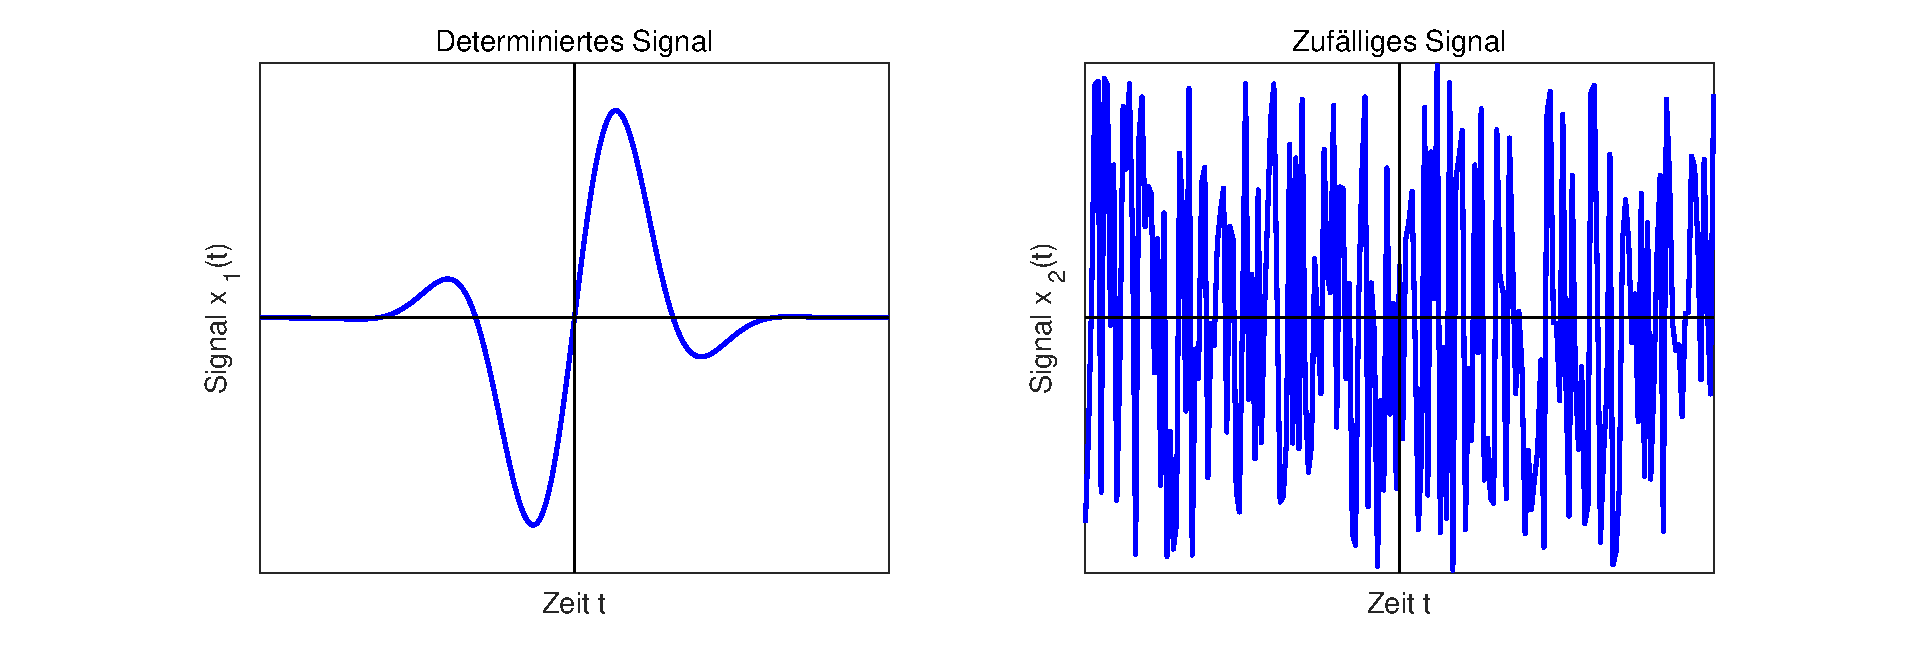
\includegraphics[width=0.5\textwidth]{Kapitel6/Bilder/image2}}
  \caption{Grafische Darstellung von Verwerfungsbereichen und Annahmebereichen f\"{u}r einen Test mit den Alternativhypothesen µ $\mathrm{>}$ µ$_{0}$, µ $\mathrm{<}$ µ$_{0}$ und µ $\neq$ µ$_{0}$}
  \label{fig:AnnahmeUndVerwerfungsbereiche}
\end{figure}

\noindent Nach der Festlegung des Verwerfungsbereichs und dem Signifikanzniveau k\"{o}nnen auf Basis der zugrunde liegenden Verteilung die Grenzen µ$_{C}$ beziehungsweise µ$_{C1}$ und µ$_{C2}$ bestimmt werden.\newline

\noindent Im einf\"{u}hrenden Beispiel zur Prozesskontrolle wurde ein zweiseitiger Test gew\"{a}hlt, da sowohl eine zu geringe, als auch eine zu gro{\ss}e Klebermenge kritisch ist. Das Signifikanzniveau von $\alpha$ = 5 \% wurde in Bild \ref{fig:DiagnoseFeuchtesensor1} \"{u}ber die blauen Fl\"{a}chen in der Wahrscheinlichkeitsdichte visualisiert.

\clearpage 

{\fontfamily{phv}\selectfont
\noindent\textbf{Schritt 5: Vergleich der Pr\"{u}fgr\"{o}{\ss}e mit den Grenzwerten}}\smallskip

\noindent F\"{u}r die konkret vorliegende Stichprobe wird abschlie{\ss}end die Pr\"{u}fgr\"{o}{\ss}e $\bar{x}$ berechnet und mit den Grenzwerten $\mu_{C}$ beziehungsweise $\mu_{C1}$ und $\mu_{C2}$ verglichen. Liegt die Pr\"{u}fgr\"{o}{\ss}e im Annahmebereich, wird die Null-Hypothese angenommen, andernfalls verworfen. \newline

\noindent In dem einleitenden Beispiel war die Pr\"{u}fverteilung eine Standardnormalverteilung. Das hat die Berechnung vergleichsweise einfach und \"{u}berschaubar gemacht. In vielen F\"{a}llen mit ausreichend gro{\ss}er Stichprobengr\"{o}{\ss}e ist es aufgrund des zentralen Grenzwertsatzes m\"{o}glich, die Normalverteilung zugrunde zu legen. 

\subsubsection{Hypothesentest mit einseitigem Verwerfungsbereich  \texorpdfstring{$\mu > \mu_{0}$}{Lg}}

\noindent Als Beispiel f\"{u}r einen Hypothesentest mit einseitigem Verwerfungsbereich $\mu > \mu_{0}$ wird der Kraftstoffverbrauch eines Fahrzeugtyps analysiert. In dem Beispiel liegen 40 Stichprobenwerte aus Fahrzeuguntersuchungen vor.\newline

\begin{table}[H]
\setlength{\arrayrulewidth}{.1em}
\caption{Beispiel zur Untersuchung des Kraftstoffverbrauchs eines Fahrzeugtyps}
\setlength{\fboxsep}{0pt}%
\colorbox{lightgray}{%
\arrayrulecolor{white}%
\begin{tabular}{wc{0cm}  wc{0.9cm} | wc{1.3cm} | wc{1.3cm} | wc{1.3cm} | wc{1.3cm} | wc{1.3cm} | wc{1.3cm} | wc{1.3cm} | wc{1.3cm} | wc{1.3cm} | wc{1.3cm}}
\hline\xrowht{15pt}

& \multicolumn{10}{c}{\fontfamily{phv}\selectfont\textbf{Benzinverbrauch V /  l/100 km}} \\ \hline \xrowht{15pt}

& 10.1 & 10.4 & 10.4 & 10.2 & 10.2 & 9.6 & 10.8 & 11.2 & 10.4 & 10.1\\ \hline\xrowht{15pt}
& 10.6 & 10.5 & 10.1 & 10.3 & 10.5 & 10.2 & 9.9 & 9.8 & 9 & 11.4\\ \hline\xrowht{15pt}
& 10.9 & 9.7 & 10.8 & 10.5 & 9.4 & 9.7 & 10.5 & 10.7 & 10 & 10.4\\ \hline\xrowht{15pt}
& 10 & 10.5 & 9.2 & 9.2 & 10.2 & 10.2 & 10.6 & 10.8 & 10.5 & 10.4\\  \hline

\end{tabular}%
}
\label{tab:sixone}
\end{table}

\noindent Es soll die Hypothese gepr\"{u}ft werden, dass die Grundgesamtheit, aus der die vorliegende Stichprobe entstammt, den Mittelwert $\mu_{0}$ = 10 l/100 km hat. Die Alternativhypothese besagt, dass er gr\"{o}{\ss}er ist. Als Signifikanzniveau wird der Wert $\alpha$ = 5 \% gew\"{a}hlt. Es wird davon ausgegangen, dass die Grundgesamtheit normalverteilt ist und eine Standardabweichung von $\sigma$ = 0.5 l/100 km aufweist.\newline

\noindent Es liegt eine Stichprobe mit bekannter Varianz vor, von der der Mittelwert getestet werden soll. Als geeignete Testgr\"{o}{\ss}e wird die Variable z gew\"{a}hlt.

\begin{equation}\label{eq:sixfourteen}
z=\dfrac{\bar{x}-\mu _{0}}{\sigma /\sqrt{N}}
\end{equation}

\noindent Nach der Aufgabenstellung soll gepr\"{u}ft werden, ob der Mittelwert µ maximal µ$_{0}$ = 10 l/100 km betr\"{a}gt. Wird der Mittelwert unterschritten, entspricht der Verbrauch trotzdem der Spezifikation. Der Verwerfungsbereich f\"{u}r die Hypothese ist deshalb µ $\mathrm{>}$ µ$_{0}$, er ist also einseitig. Damit kann die Aufgabe mithilfe der Wahrscheinlichkeitsdichte veranschaulicht werden, die ist in Bild \ref{fig:HypothesentestRechterVerwerfungsbereich} dargestellt.

\clearpage 

\noindent 
\begin{figure}[H]
  \centerline{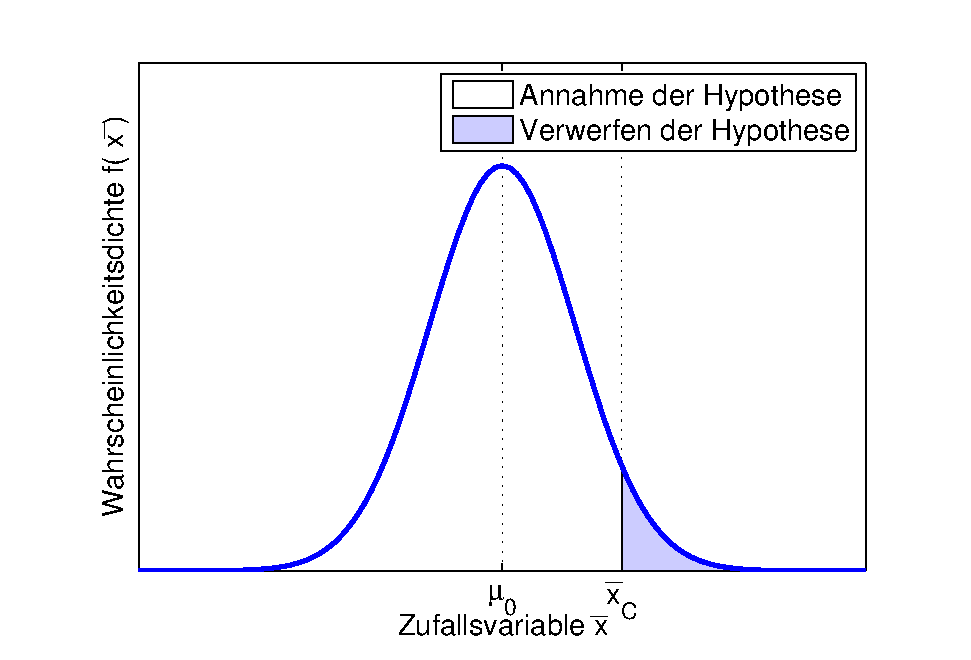
\includegraphics[width=0.5\textwidth]{Kapitel6/Bilder/image3}}
  \caption{Darstellung des Hypothesentests mit einseitigem Verwerfungsbereich µ $\mathrm{>}$ µ$_{0}$}
  \label{fig:HypothesentestRechterVerwerfungsbereich}
\end{figure}

\noindent Damit ein Stichprobenwert $\overline{\mathrm{x}}$ mit einer Sicherheit von 95 \% nicht zu der Normalverteilung geh\"{o}rt, muss er f\"{u}r diese Aufgabenstellung in dem Bereich der blauen Fl\"{a}che unter der Kurve liegen. Die Fl\"{a}che repr\"{a}sentiert die Wahrscheinlichkeit von 5 \%.\newline

\noindent Mit dieser Verteilung wird die Wahrscheinlichkeit $\gamma$, mit der die Variable z im Annahmebereich liegt, definiert als

\begin{equation}\label{eq:sixfifteen}
\gamma =1-\alpha =P(z<c)=F(c)
\end{equation}

\noindent Bei Annahme eines einseitigen Tests mit dem Verwerfungsbereich µ $\mathrm{>}$ µ$_{0}$ ergibt sich die Konstante c aus der Bedingung

\begin{equation}\label{eq:sixsixteen}
F\left(c\right)=1-\alpha =\gamma
\end{equation}

\noindent Aufl\"{o}sen nach c f\"{u}hrt zu

\begin{equation}\label{eq:sixseventeen}
c=F^{-1} (1-\alpha)
\end{equation}

\noindent Durch Umformungen von Gleichung \eqref{eq:sixfifteen} ergibt sich ein Ausdruck f\"{u}r den Annahmebereich der Nullhypothese, n\"{a}mlich dass der gesch\"{a}tzte Mittelwert $\overline{\mathrm{x}}$, mit einer spezifizierten Wahrscheinlichkeit $\gamma$, zu der Normalverteilung mit dem Mittelwert µ$_{0}$ und der Varianz $\sigma^{2}$/N geh\"{o}rt.

\begin{equation}\label{eq:sixeighteen}
\gamma =P\left(\dfrac{\bar{x}-\mu _{0} }{\sigma /\sqrt{N} } <c\right)=P\left(\bar{x}<\mu _{0} +\dfrac{c\cdot \sigma }{\sqrt{N} } \right)
\end{equation}

\noindent Die Konstante c ergibt sich zu 

\begin{equation}\label{eq:sixnineteen}
c=1.6449
\end{equation}

\noindent Damit ergibt sich der Annahmebereich zu

\begin{equation}\label{eq:sixtwenty}
\bar{x}<\mu _{0} +\dfrac{c\cdot \sigma }{\sqrt{N}} =10+\dfrac{1.6449\cdot 0.5}{\sqrt{40}} =10.13
\end{equation}

\noindent Der Mittelwert der vorliegenden Stichprobe liegt bei ${\overline{\mathrm{x}}}_0$ = 10.25 l/100 km und somit im Verwerfungsbereich des Hypothesentests.\noindent

\noindent Bei dem vorgestellten Test wird aus dem Signifikanzniveau $\alpha$ die Grenze µ$_{C}$ f\"{u}r die Pr\"{u}fgr\"{o}{\ss}e $\overline{\mathrm{x}}$ berechnet. Die Berechnung erfolgt \"{u}ber die zugrundeliegende Wahrscheinlichkeitsverteilung. Bei dieser Form des Hypothesentest kann nur ausgesagt werden, ob die Hypothese angenommen oder verworfen wird. Es fehlt eine quantitative Bewertung. Alternativ kann eine \"{U}berschreitungswahrscheinlichkeit p der Pr\"{u}fgr\"{o}{\ss}e ${\overline{\mathrm{x}}}_0$ bestimmt werden und mit dem Signifikanzniveau $\alpha$ verglichen werden. Diese Art des Tests ist standardm\"{a}{\ss}ig in statistischen Software-Paketen implementiert, da sie eine quantitative Bewertung erm\"{o}glicht. Bei Hypothesentests mit einseitigem Verwerfungsbereich µ $\mathrm{>}$ µ$_{0}$ muss f\"{u}r die Annahme der Nullhypothese die Bedingung

\begin{equation}\label{eq:sixtwentyone}
p=1-F(\bar{x}_{0})>\alpha
\end{equation}

\noindent erf\"{u}llt werden. Je gr\"{o}{\ss}er der Wert p ist, desto sicherer wird die Hypothese H$_{0}$ best\"{a}tigt. Bild \ref{fig:HypothesentestRechterVerwerfungsbereichPvalue} stellt die \"{U}berschreitungswahrscheinlichkeit p grafisch dar. 

\noindent 
\begin{figure}[H]
  \centerline{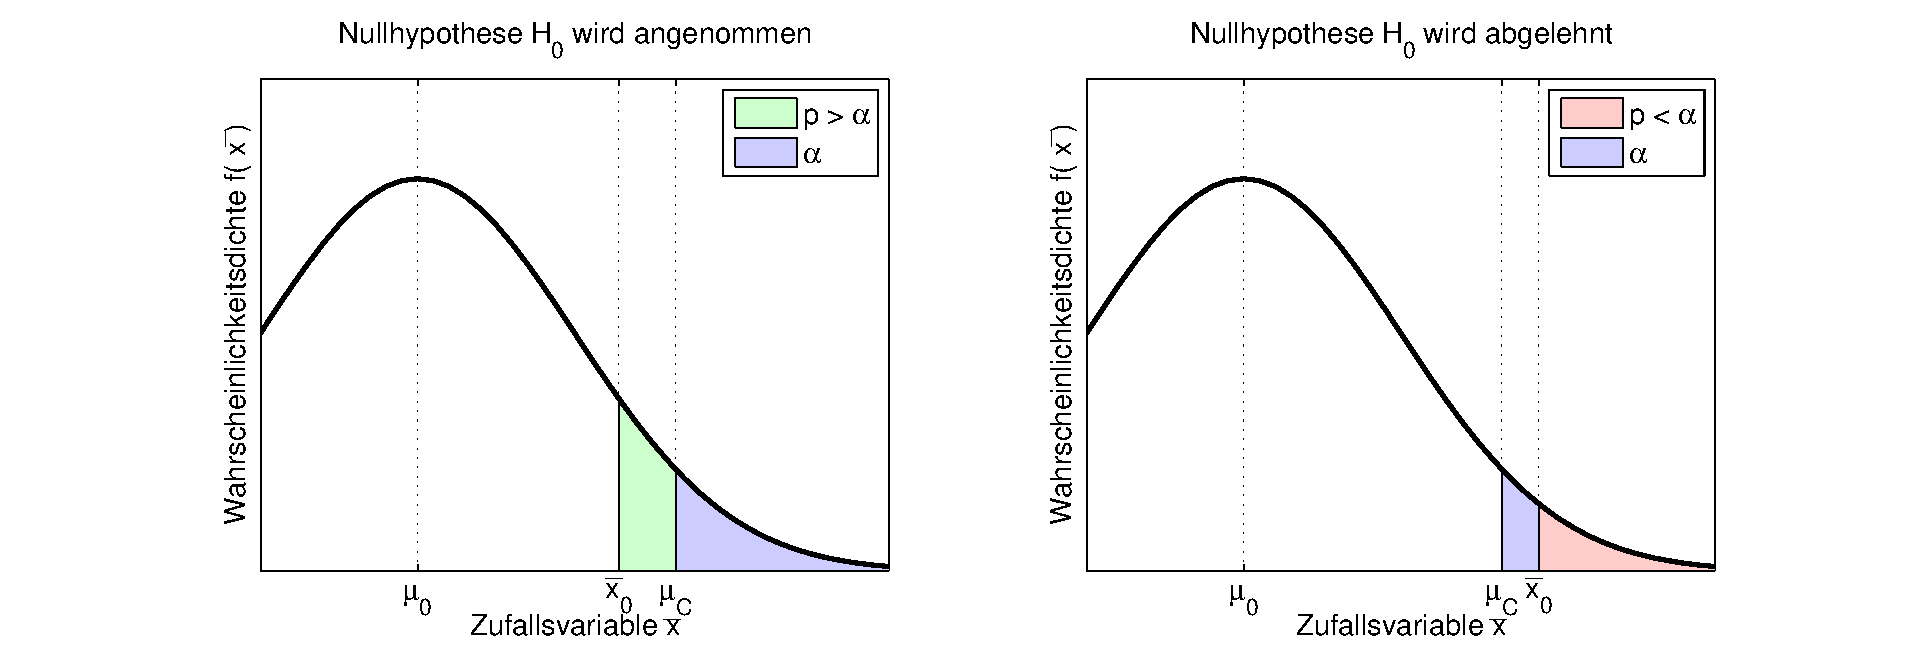
\includegraphics[width=1\textwidth]{Kapitel6/Bilder/image4}}
  \caption{\"{U}berschreitungswahrscheinlichkeit p beim Hypothesentest mit einseitigem Verwerfungsbereich µ $\mathrm{>}$ µ$_{0}$}
  \label{fig:HypothesentestRechterVerwerfungsbereichPvalue}
\end{figure}

\noindent F\"{u}r das Beispiel ergibt sich ein p-Wert aus der Standardnormalverteilung von

\begin{equation}\label{eq:sixtwentytwo}
p=1-F\left(\dfrac{\bar{x}-\mu _{0}}{\sigma /\sqrt{N}} \right)=1-F\left(\dfrac{10.25-10}{0.5/\sqrt{40} } \right)= 7.827\cdot 10^{-4} <0.05 = \alpha
\end{equation}

\noindent Der Wert liegt deutlich unter der Grenze von 5 \%, sodass die Nullhypothese verworfen werden muss. Der Kraftstoffverbrauch des Fahrzeugtyps liegt demnach statistisch gesehen \"{u}ber dem Spezifikationsbereich von 10 l/100 km.  

\subsubsection{Hypothesentest mit einseitigem Verwerfungsbereich \texorpdfstring{$\mu < \mu_{0}$}{Lg}}

\noindent Als Beispiel f\"{u}r einen Hypothesentest mit einseitigem Verwerfungsbereich $\mu < \mu_{0}$ wird die Zugfestigkeit von Folien untersucht. Dazu sind 30 Messwerte aus Zugversuchen gegeben, die in Tabelle \ref{tab:sixtwo} dargestellt sind.

\begin{table}[H]
\setlength{\arrayrulewidth}{.1em}
\caption{Beispiel zur Untersuchung der Zugfestigkeit von Folien}
\setlength{\fboxsep}{0pt}%
\colorbox{lightgray}{%
\arrayrulecolor{white}%
\begin{tabular}{wc{0.4cm}  wl{1.7cm} | wc{2.5cm} | wc{2.5cm} | wc{2.5cm} | wc{2.5cm} | wc{2.5cm} | wc{2.5cm} }
\hline\xrowht{15pt}

& \multicolumn{6}{c}{\fontfamily{phv}\selectfont\textbf{Zugfestigkeit $\beta_{Z}$  /  N/cm$^{2}$}} \\ \hline \xrowht{15pt}

& 44.00 & 44.50 & 44.50 & 44.40 & 42.50 & 40.80\\ \hline\xrowht{15pt}
& 43.30 & 43.50 & 46.70 & 44.90 & 43.90 & 43.70\\ \hline\xrowht{15pt}
& 42.90 & 44.10 & 42.00 & 44.00 & 44.80 & 43.50\\ \hline\xrowht{15pt}
& 43.80 & 43.80 & 42.80 & 44.30 & 41.10 & 45.80\\ \hline\xrowht{15pt}
& 43.20 & 44.20 & 42.50 & 46.10 & 44.50 & 43.20\\ \hline

\end{tabular}%
}
\label{tab:sixtwo}
\end{table}

\noindent Es soll die Hypothese gepr\"{u}ft werden, dass die Grundgesamtheit, aus der die Stichprobe von Messwerten genommen wurde, einen Mittelwert µ$_{0}$ $\geq$ 44 N/cm$^{2}$ hat. Es wird davon ausgegangen, dass die Grundgesamtheit normalverteilt ist und eine Standardabweichung von $\sigma$ = 1.29 N/cm² aufweist. Als Signifikanzniveau wird der Wert $\alpha$ = 5 \% gefordert.\newline

\noindent Es liegt eine Stichprobe mit bekannter Varianz vor, von der der Mittelwert getestet werden soll. Als geeignete Testgr\"{o}{\ss}e wird wieder die Variable z gew\"{a}hlt.

\begin{equation}\label{eq:sixtwentythree}
z=\dfrac{\bar{x}-\mu _{0}}{\sigma /\sqrt{N}}
\end{equation}

\noindent Nach der Aufgabenstellung soll gepr\"{u}ft werden, ob der Mittelwert µ mindestens µ$_{0}$ = 44 N/cm$^{2}$ betr\"{a}gt. Wird der Mittelwert \"{u}berschritten, entspricht die Folie trotzdem der Spezifikation. Der Verwerfungsbereich f\"{u}r die Hypothese ist deshalb µ $\mathrm{<}$ µ$_{0}$, er ist also einseitig.\newline

\noindent Wieder wird die Aufgabe mithilfe der Wahrscheinlichkeitsdichte veranschaulicht, sie ist in Bild \ref{fig:HypothesentestLinkerVerwerfungsbereich} dargestellt.

\noindent 
\begin{figure}[H]
  \centerline{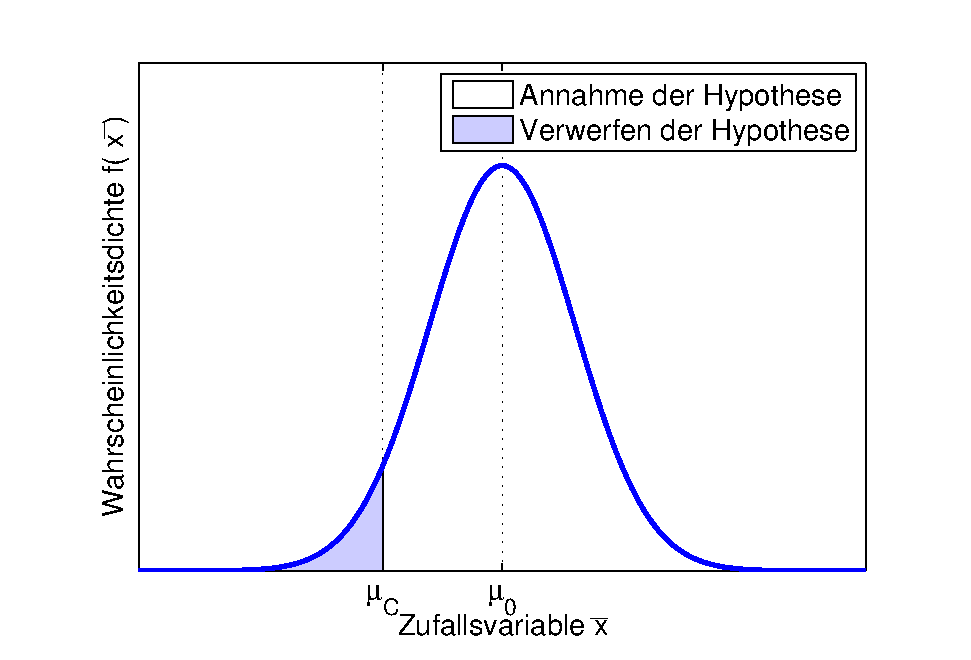
\includegraphics[width=0.5\textwidth]{Kapitel6/Bilder/image5}}
  \caption{Darstellung des Hypothesentests mit einseitigem Verwerfungsbereich µ $\mathrm{<}$ µ$_{0}$}
  \label{fig:HypothesentestLinkerVerwerfungsbereich}
\end{figure}

\noindent Damit ein Stichprobenwert $\overline{\mathrm{x}}$ mit einer Sicherheit von 95 \% nicht zu der Normalverteilung geh\"{o}rt, muss er f\"{u}r diese Aufgabenstellung in dem Bereich der blauen Fl\"{a}che unter der Kurve liegen. Die Fl\"{a}che repr\"{a}sentiert die Wahrscheinlichkeit von 5 \%. \newline

\noindent Mit dieser Verteilung wird wieder die Wahrscheinlichkeit $\gamma$, mit der die Variable z im Annahmebereich liegt, definiert als

\begin{equation}\label{eq:sixtwentyfour}
\gamma =1-\alpha =P(c<z)=1-F(c)
\end{equation}

\noindent Bei Annahme eines einseitigen Tests mit dem Verwerfungsbereich µ $\mathrm{<}$ µ$_{0}$ ergibt sich die Konstante c aus der Bedingung

\begin{equation}\label{eq:sixtwentyfive}
F(c)=1-\gamma =\alpha
\end{equation}

\noindent Aufl\"{o}sen nach c f\"{u}hrt zu

\begin{equation}\label{eq:sixtwentysix}
c=F^{-1} (\alpha)
\end{equation}

\noindent Durch Umformungen von Gleichung \eqref{eq:sixtwentyfour} ergibt sich ein Ausdruck f\"{u}r den Annahmebereich der Nullhypothese, dass der gesch\"{a}tzter Mittelwert $\overline{\mathrm{x}}$ mit einer spezifizierten Wahrscheinlichkeit $\gamma$ zu der Normalverteilung mit dem Mittelwert µ$_{0}$ und der Varianz $\sigma^{2}$/N geh\"{o}rt.

\begin{equation}\label{eq:sixtwentyseven}
\gamma =P\left(c<\dfrac{\bar{x}-\mu _{0} }{\sigma /\sqrt{N}} \right)=P\left(\mu _{0} +\dfrac{c\cdot \sigma }{\sqrt{N}} <\bar{x}\right)
\end{equation}

\noindent Die Konstante c ergibt sich zu

\begin{equation}\label{eq:sixtwentyeight}
c=-1.6449
\end{equation}

\noindent Damit lautet der Annahmebereich 

\begin{equation}\label{eq:sixtwentynine}
\bar{x}>\mu _{0} +\dfrac{c\cdot \sigma}{\sqrt{N}} =44-\dfrac{1.6449\cdot 1.29}{\sqrt{30}} =43.6126
\end{equation}

\noindent Der Mittelwert der vorliegenden Stichprobe liegt bei ${\overline{\mathrm{x}}}_0$ = 43.78 N/cm² und somit im Annahmebereich des Hypothesentests.

\noindent Alternativ kann wie im Abschnitt zuvor eine Unterschreitungswahrscheinlichkeit p der Pr\"{u}fgr\"{o}{\ss}e $\overline{\mathrm{x}}$ bestimmt werden und mit dem Signifikanzniveau $\alpha$ verglichen werden. Diese Art des Tests ist wie bereits erw\"{a}hnt standardm\"{a}{\ss}ig in statistischen Software-Paketen implementiert, da sie eine quantitative Bewertung erm\"{o}glicht. Bei Hypothesentests mit einseitigem Verwerfungsbereich µ $\mathrm{<}$ µ$_{0}$ muss f\"{u}r die Annahme der Nullhypothese die Bedingung

\begin{equation}\label{eq:sixthirty}
p=F(\bar{x}_{0})>\alpha
\end{equation}

\noindent erf\"{u}llt werden. Je gr\"{o}{\ss}er der Wert p ist, desto sicherer wird die Hypothese H$_{0}$ best\"{a}tigt. Bild \ref{fig:HypothesentestLinkerVerwerfungsbereichPvalue} stellt die \"{U}berschreitungswahrscheinlichkeit p grafisch dar. 

\noindent 
\begin{figure}[H]
  \centerline{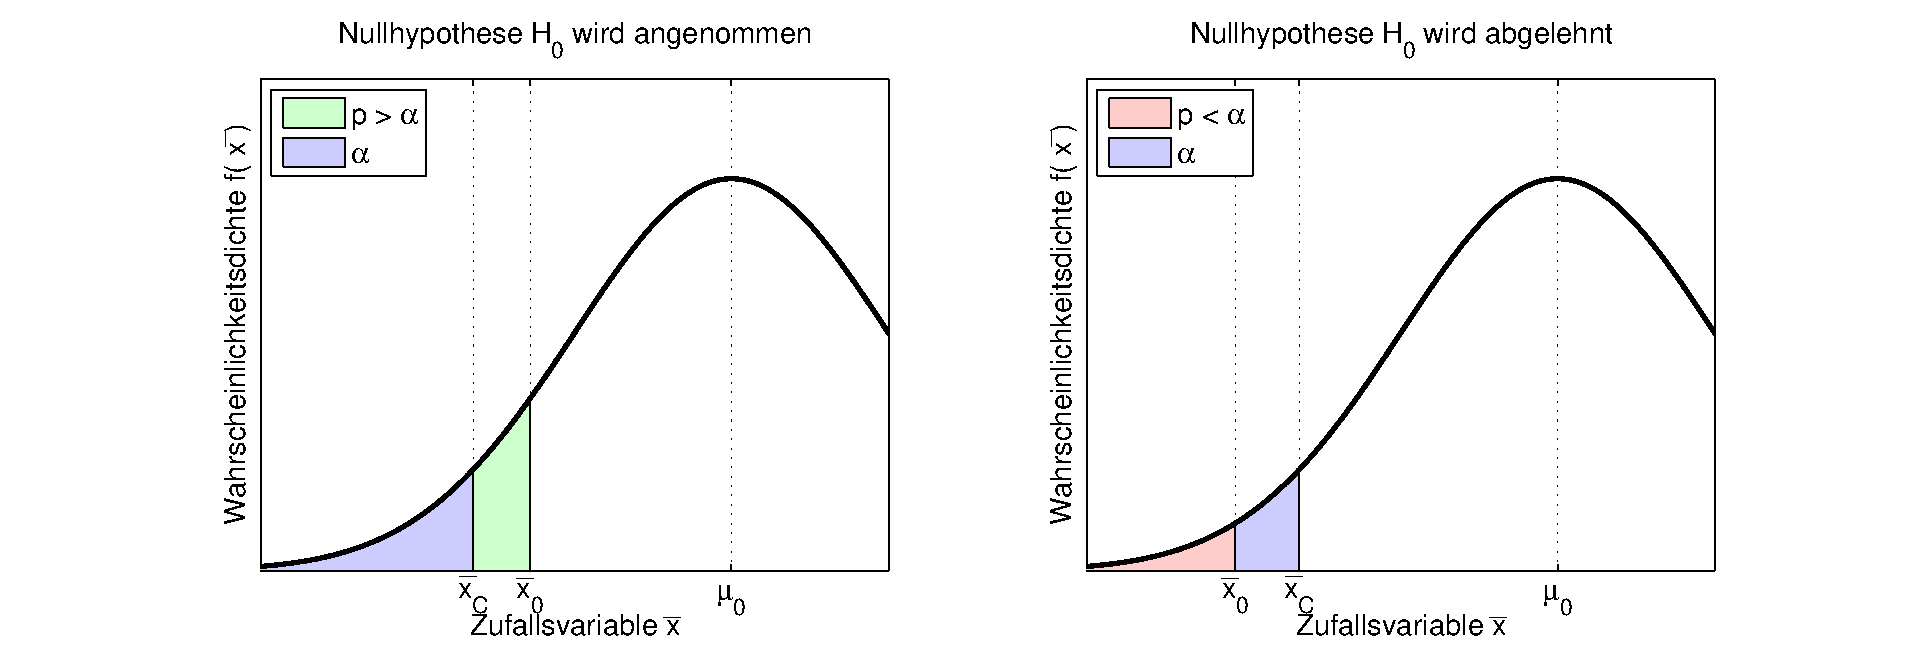
\includegraphics[width=1\textwidth]{Kapitel6/Bilder/image6}}
  \caption{\"{U}berschreitungswahrscheinlichkeit p beim Hypothesentest mit einseitigem Verwerfungsbereich µ $\mathrm{<}$ µ$_{0}$}
  \label{fig:HypothesentestLinkerVerwerfungsbereichPvalue}
\end{figure}

\noindent F\"{u}r das Beispiel ergibt sich ein p-Wert von

\begin{equation}\label{eq:sixthirtyone}
p=F\left(\dfrac{\bar{x}_{0} -\mu _{0} }{\sigma /\sqrt{N} } \right)=F\left(\dfrac{43.78-44}{1.29/\sqrt{30} } \right)={\rm 0.1751}>0.05=\alpha
\end{equation}

\noindent Die Bedingung f\"{u}r eine Annahme der Nullhypothese ist damit erf\"{u}llt.

\clearpage

\subsubsection{Hypothesentest mit zweiseitigem Verwerfungsbereich \texorpdfstring{$\mu \neq \mu_{0}$}{Lg}}

\noindent Der Fall eines Hypothesentests mit zweiseitigem Verwerfungsbereich $\mu \neq \mu_{0}$ wird an dem Beispiel von Drehteilen diskutiert. Dazu sind 20 Drehteile vermessen worden, deren Durchmesser in Tabelle \ref{tab:sixthree} dargestellt sind.

\begin{table}[H]
\setlength{\arrayrulewidth}{.1em}
\caption{Beispiel zur Untersuchung der Ma{\ss}haltigkeit von Drehteilen}
\setlength{\fboxsep}{0pt}%
\colorbox{lightgray}{%
\arrayrulecolor{white}%
\begin{tabular}{wc{0.7cm}  wl{1.9cm} | wc{3cm} | wc{3cm} | wc{3cm} | wc{3cm} | wc{3cm} }
\hline\xrowht{15pt}

& \multicolumn{5}{c}{\fontfamily{phv}\selectfont\textbf{Durchmesser Drehteile d / mm}} \\ \hline \xrowht{15pt}

& 50.89 & 51.01 & 50.94 & 50.84 & 50.27\\ \hline\xrowht{15pt}
& 50.36 & 50.09 & 50.80 & 50.47 & 50.94\\ \hline\xrowht{15pt}
& 50.69 & 50.70 & 50.57 & 50.06 & 50.51\\ \hline\xrowht{15pt}
& 50.66 & 51.07 & 50.50 & 50.48 & 50.64\\ \hline

\end{tabular}%
}
\label{tab:sixthree}
\end{table}

\noindent Es soll die Hypothese gepr\"{u}ft werden, dass die Grundgesamtheit, aus der die Stichprobe von Fertigungsteilen genommen wurde, einen Mittelwert µ$_{0}$ = 50.55 mm hat. Die Gegenhypothese ist, dass der Mittelwert signifikant davon abweicht. Es wird davon ausgegangen, dass die Grundgesamtheit normalverteilt ist und eine Standardabweichung von $\sigma$ = 0.29 mm aufweist. Als Signifikanzniveau wird der Wert $\alpha$ = 5 \% gefordert.\newline

\noindent Es liegt wieder eine Stichprobe mit bekannter Varianz vor, von der der Mittelwert getestet werden soll. Als geeignete Testgr\"{o}{\ss}e wird die Variable z gew\"{a}hlt.

\begin{equation}\label{eq:sixthirtytwo}
z=\dfrac{\bar{x}-\mu _{0} }{\sigma /\sqrt{N} }
\end{equation}

\noindent Nach der Aufgabenstellung soll gepr\"{u}ft werden, ob der Mittelwert µ genau µ$_{0}$ = 50.55 mm betr\"{a}gt. Der Verwerfungsbereich f\"{u}r die Hypothese ist µ $\neq$ µ$_{0}$, er ist also zweiseitig. Auch in diesem Fall kann die Aufgabe mithilfe der Wahrscheinlichkeitsdichte veranschaulicht werden, die ist in Bild \ref{fig:HypothesentestBeidseitigerVerwerfungsbereich} dargestellt.

\noindent 
\begin{figure}[H]
  \centerline{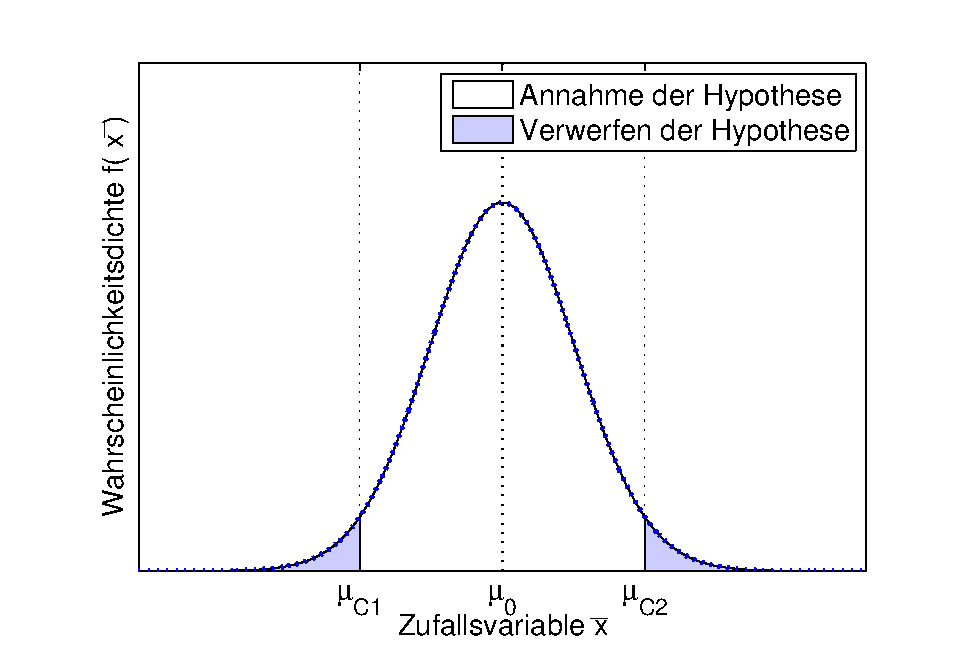
\includegraphics[width=0.5\textwidth]{Kapitel6/Bilder/image7}}
  \caption{Darstellung des Hypothesentests mit zweiseitigem Verwerfungsbereich µ $\neq$ µ$_{0}$}
  \label{fig:HypothesentestBeidseitigerVerwerfungsbereich}
\end{figure}

\noindent Damit ein Stichprobenwert $\overline{\mathrm{x}}$ mit einer Sicherheit von 95 \% nicht zu der Normalverteilung mit dem Mittelwert µ{}$_{0}$ und der Varianz $\sigma^{2}$/N geh\"{o}rt, muss er f\"{u}r diese Aufgabenstellung in dem Bereich der blauen Fl\"{a}che unter der Kurve liegen. Die Fl\"{a}che repr\"{a}sentiert insgesamt die Wahrscheinlichkeit von 5~\%, ist in diesem Fall aber in zwei Bereiche von jeweils 2.5 \% aufgeteilt. \newline

\noindent Mit dieser Verteilung wird nach Gleichung \eqref{eq:sixone} die Wahrscheinlichkeit $\gamma$, mit der die Variable z im Annahmebereich liegt, definiert als

\begin{equation}\label{eq:sixthirtythree}
\gamma =1-\alpha =P(c_{1} <z\le c_{2})=F(c_{2} )-F(c_{1})
\end{equation}

\noindent Bei Annahme eines zweiseitigen Tests mit dem Verwerfungsbereich µ $\neq$ µ$_{0}$ ergeben sich die Konstanten c$_{1}$ und c$_{2}$ aus den Bedingungen

\begin{equation}\label{eq:sixthirtyfour}
F(c_{1})=\dfrac{1-\gamma}{2} =\dfrac{\alpha}{2}
\end{equation}
\begin{equation}\label{eq:sixthirtyfive}
F(c_{2})=1-\dfrac{1-\gamma}{2} =1-\dfrac{\alpha}{2}
\end{equation}

\noindent Aufl\"{o}sen nach den Konstanten c$_{1}$ und c$_{2}$ f\"{u}hrt zu

\begin{equation}\label{eq:sixthirtysix}
c_{1} =F^{-1} \left(\dfrac{\alpha }{2} \right)
\end{equation}
\begin{equation}\label{eq:sixthirtyseven}
c_{2} =F^{-1} \left(1-\dfrac{\alpha }{2} \right)
\end{equation}

\noindent Durch Umformungen von Gleichung \eqref{eq:sixthirtythree} ergibt sich ein Ausdruck f\"{u}r den Annahmebereich der Nullhypothese, dass der gesch\"{a}tzter Mittelwert $\overline{\mathrm{x}}$ mit einer spezifizierten Wahrscheinlichkeit $\gamma$ zu der Normalverteilung mit dem Mittelwert µ$_{0}$ und der Varianz $\sigma^{2}$/N geh\"{o}rt.

\begin{equation}\label{eq:sixthirtyeight}
\gamma =P\left(c_{1} <\dfrac{\bar{x}-\mu _{0}}{\sigma /\sqrt{N}} \le c_{2} \right)=P\left(\mu _{0} +\dfrac{c_{1} \cdot \sigma }{\sqrt{N}} <\bar{x}\le \mu _{0} +\dfrac{c_{2} \cdot \sigma }{\sqrt{N}} \right)
\end{equation}

\noindent Die Konstante c$_{1}$ und c$_{2}$ ergeben sich zu

\begin{equation}\label{eq:sixthirtynine}
c_{1} =-1.96
\end{equation}
\begin{equation}\label{eq:sixfourty}
c_{2} =1.96
\end{equation}

\noindent Damit ergibt sich der Annahmebereich in diesem Beispiel zu

\begin{equation}\label{eq:sixfourtyone}
\mu _{0} +\dfrac{c_{1} \cdot \sigma }{\sqrt{N}} = 50.55-\dfrac{1.96\cdot 0.29}{\sqrt{20}} =50.42<\bar{x}\le 50.68= 50.55-\dfrac{1.96\cdot 0.29}{\sqrt{20}} =\mu _{0} +\dfrac{c_{2} \cdot \sigma}{\sqrt{N}}
\end{equation}

\noindent Der Mittelwert der vorliegenden Stichprobe liegt bei ${\overline{\mathrm{x}}}_0$ = 50.62 mm und somit im Annahmebereich des Hypothesentests.

\clearpage

\noindent Alternativ kann wie im Abschnitt zuvor eine Unterschreitungswahrscheinlichkeit p der Pr\"{u}fgr\"{o}{\ss}e ${\overline{\mathrm{x}}}_0$ bestimmt werden und mit dem Signifikanzniveau $\alpha$ verglichen werden. Bei Hypothesentests mit beidseitigem Verwerfungsbereich µ $\neq$ µ$_{0}$ m\"{u}ssen die Bedingungen

\begin{equation}\label{eq:sixfourtytwo}
p=F\left(\bar{x}_{0} \right)>\dfrac{\alpha }{2}
\end{equation}

\noindent und

\begin{equation}\label{eq:sixfourtythree}
p=F(\bar{x}_{0})<1-\dfrac{\alpha}{2}
\end{equation}

\noindent erf\"{u}llt werden. Je zentraler der Wert p zwischen den Grenzen $\alpha$/2 und 1 - $\alpha$/2 liegt, desto sicherer wird die Hypothese H$_{0}$ best\"{a}tigt. Bild \ref{fig:HypothesentestBeidseitigerVerwerfungsbereichPvalue} stellt die \"{U}berschreitungswahrscheinlichkeit p mit den unterschiedlichen Annahme- und Verwerfungsszenarien grafisch dar. 

\noindent 
\begin{figure}[H]
  \centerline{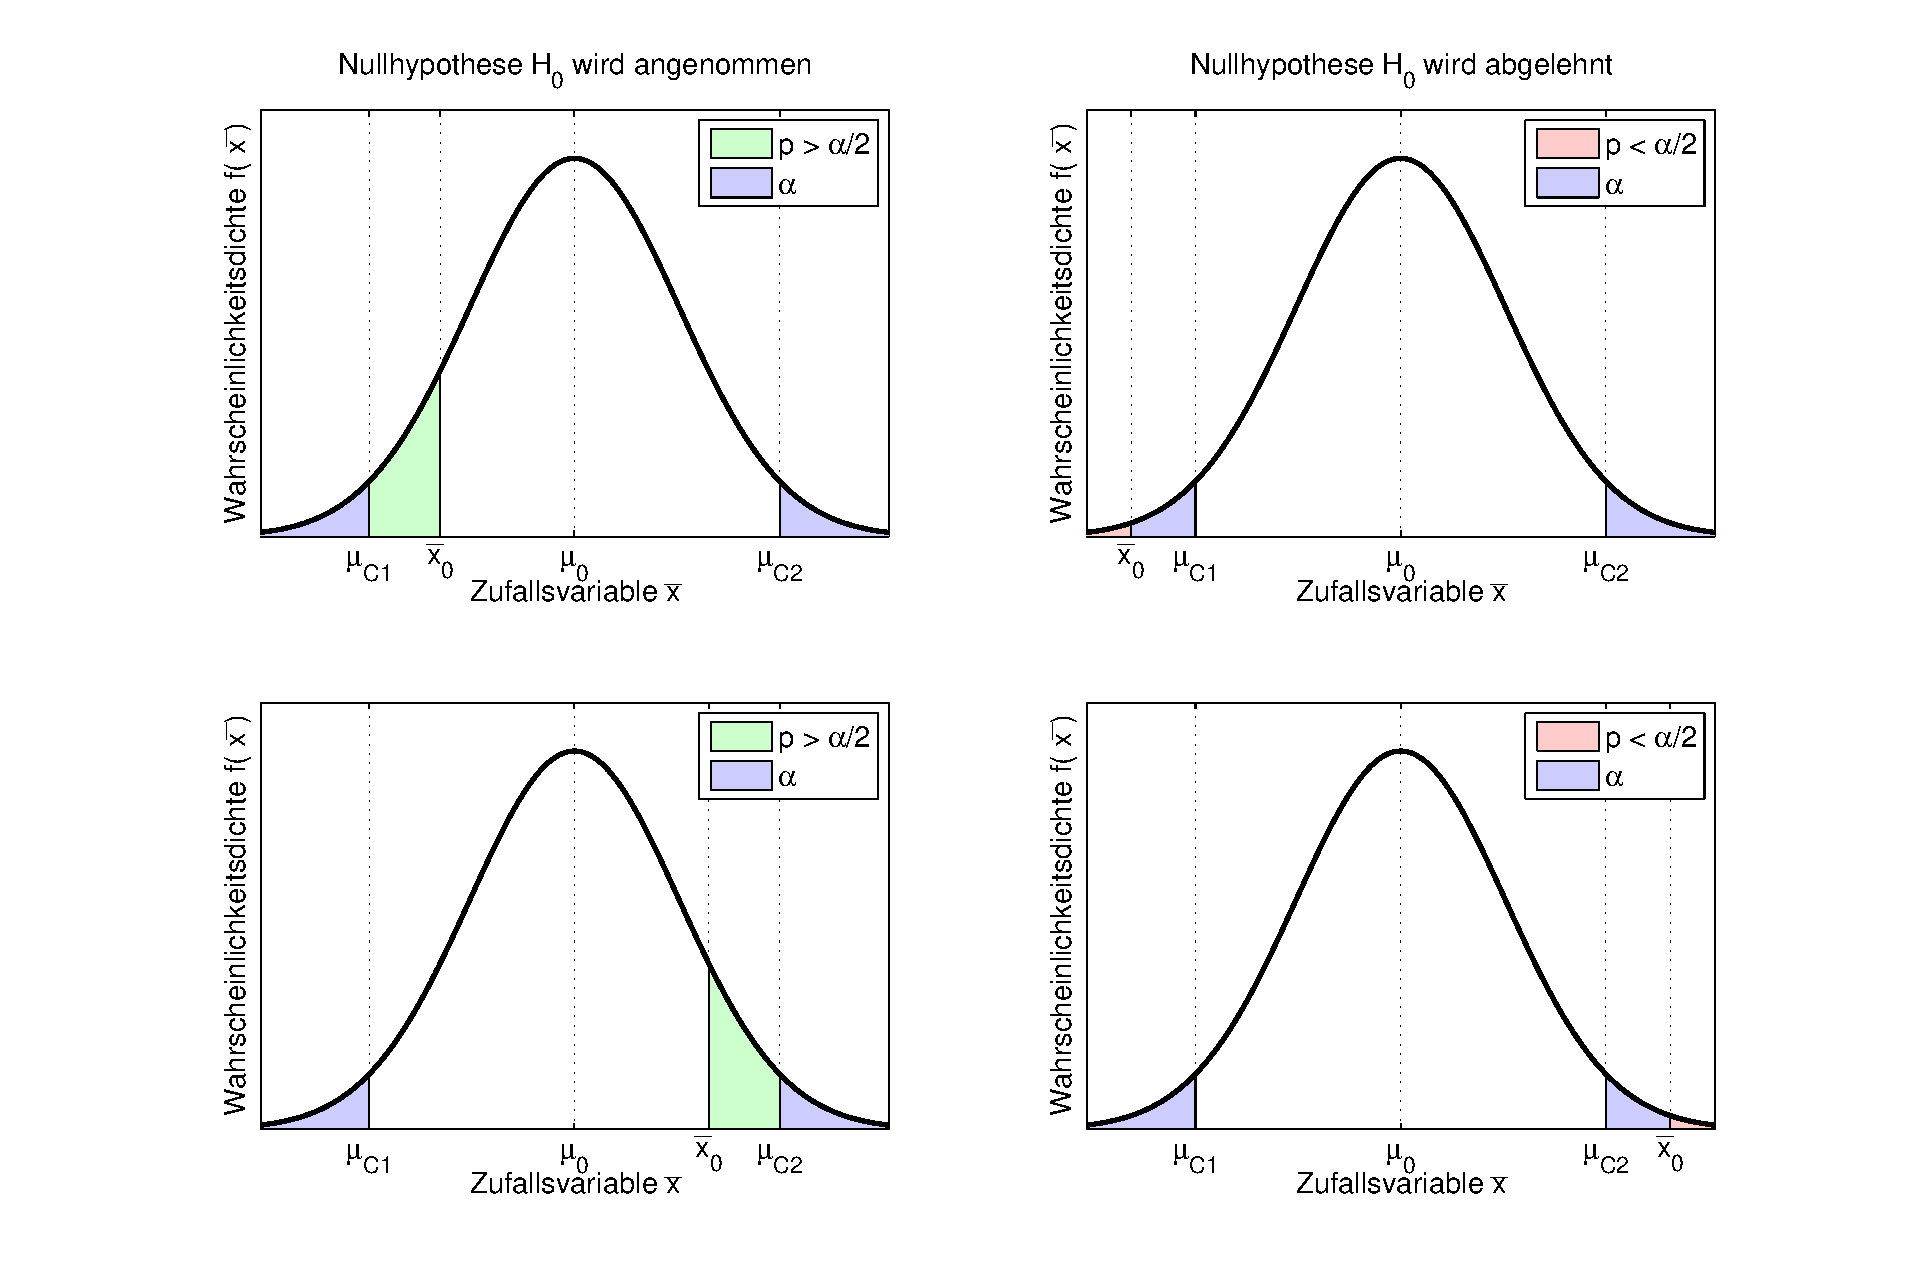
\includegraphics[width=1\textwidth]{Kapitel6/Bilder/image8}}
  \caption{\"{U}berschreitungswahrscheinlichkeit p beim Hypothesentest mit zweiseitigem Verwerfungsbereich µ $\neq$ µ${}_{0}$}
  \label{fig:HypothesentestBeidseitigerVerwerfungsbereichPvalue}
\end{figure}

\noindent Mit dem Mittelwert der vorliegenden Stichprobe von ${\overline{\mathrm{x}}}_0$ = 50.62 mm ergibt sich ein p-Wert von 

\begin{equation}\label{eq:sixfourtyfour}
p=F\left(\dfrac{\bar{x}_{0} -\mu _{0}}{\sigma /\sqrt{N}} \right)=F\left(\dfrac{50.62-50.55}{0.29/\sqrt{20}} \right)=0.8598
\end{equation}

\noindent Damit wird die Hypothese, dass die Grundgesamtheit einen Durchmesser von 50.55 mm besitzt, angenommen.

\clearpage

\subsection{Hypothesentest und Konfidenzbereich}

\noindent Bei einigen statistischen Verfahren wird statt des Hypothesentests eine Analyse des Konfidenzbereichs durchgef\"{u}hrt. Das Vorgehen zur Berechnung der Konfidenzbereiche und das Vorgehen zum Hypothesentest entsprechen einander. Beide Verfahren werden im Folgenden am Beispiel des Mittelwertes einer Grundgesamtheit mit bekannter Varianz miteinander verglichen.


\subsubsection{Hypothesentest}

\noindent Beim Hypothesentest wird gepr\"{u}ft, ob der Mittelwert einer vorliegenden Stichprobe mit der Wahrscheinlichkeit $\gamma$ in dem Annahmebereich mit den Grenzen µ$_{C1}$ und µ$_{C2}$ liegt. 

\begin{equation}\label{eq:sixfourtyfive}
\gamma =1-\alpha =P\left(\mu _{C1} <\bar{x}\le \mu _{C2} \right)
\end{equation}

\noindent Die Berechnung der Grenzen µ$_{C1}$ und µ$_{C2}$ beruht darauf, eine Zufallsvariable mit einer bekannten Verteilung zu finden, in deren Beschreibung die Hypothese H$_{0}$ und der bekannte Parameter der Stichprobe vorkommen. F\"{u}r das Beispiel des Mittelwertes gilt dies f\"{u}r die standardnormalverteilte Zufallsvariable

\begin{equation}\label{eq:sixfourtysix}
z=\dfrac{\bar{x}-\mu _{0}}{\sigma /\sqrt{N}}
\end{equation}

\noindent Mit dieser Verteilung wird nach Gleichung \eqref{eq:sixfourtyfive} die Wahrscheinlichkeit $\gamma$, mit der die Variable z innerhalb des Intervalls c$_{1}$ {\dots} c$_{2}$ liegt, definiert als

\begin{equation}\label{eq:sixfourtyseven}
\gamma =P\left(c_{1} <z\le c_{2} \right)=F(c_{2})-F(c_{1})
\end{equation}

\noindent Durch Umformungen von Gleichung \eqref{eq:sixfourtyseven} ergibt sich ein Ausdruck f\"{u}r den Annahmebereich der Nullhypothese, dass der vorliegende Mittelwert ${\overline{\mathrm{x}}}_0$ mit einer spezifizierten Wahrscheinlichkeit $\gamma$ zu der Normalverteilung mit dem Mittelwert µ$_{0}$ und der Varianz $\sigma^{2}$/N geh\"{o}rt.

\begin{equation}\label{eq:sixfourtyeight}
\gamma =P\left(c_{1} <\dfrac{\bar{x}_{0} -\mu _{0}}{\sigma /\sqrt{N}} \le c_{2} \right)=P\left(\mu _{0} +\dfrac{c_{1} \cdot \sigma }{\sqrt{N} } <\bar{x}_{0} \le \mu _{0} +\dfrac{c_{2} \cdot \sigma }{\sqrt{N}} \right)=P\left(\mu _{C1} <\bar{x}_{0} \le \mu _{C2} \right)
\end{equation}

\noindent Liegt er innerhalb des Annahmebereiches, wird die Hypothese angenommen, andernfalls abgelehnt.

\subsubsection{Konfidenzbereich}

\noindent Beim Konfidenzbereich wird auf Grundlage einer vorliegenden Stichprobe berechnet, in welchem Intervall der Mittelwert $\mu$ der Grundgesamtheit liegt. 

\begin{equation}\label{eq:sixfourtynine}
\gamma =1-\alpha =P\left(\mu _{C1} <\mu \le \mu _{C2} \right)
\end{equation}

\noindent Die Berechnung der Grenzen µ$_{C1}$ und µ$_{C2}$ beruht darauf, eine Zufallsvariable mit einer bekannten Verteilung zu finden, in deren Beschreibung der Parameter der Grundgesamtheit und der bekannte Parameter der Stichprobe vorkommen. F\"{u}r das Beispiel des Mittelwertes gilt dies f\"{u}r die standardnormalverteilte Zufallsvariable

\begin{equation}\label{eq:sixfifty}
z=\dfrac{\bar{x}-\mu}{\sigma /\sqrt{N}}
\end{equation}

\noindent Mit dieser Verteilung wird nach Gleichung \eqref{eq:sixfourtynine} die Wahrscheinlichkeit $\gamma$, mit der die Variable z innerhalb des Intervalls c$_{1}$ {\dots} c$_{2}$ liegt, definiert als

\begin{equation}\label{eq:sixfiftyone}
\gamma =P(c_{1} <z\le c_{2})=F(c_{2})-F(c_{1})
\end{equation}

\noindent Durch Umformungen von Gleichung \eqref{eq:sixfiftyone} ergibt sich ein Ausdruck f\"{u}r Konfidenzbereich des Mittelwertes der Grundgesamtheit.

\begin{equation}\label{eq:sixfiftytwo}
\gamma =P\left(c_{1} <\dfrac{\bar{x}-\mu }{\sigma /\sqrt{N}} \le c_{2} \right)=P\left(\bar{x}-\dfrac{c_{2} \cdot \sigma }{\sqrt{N}} <\mu \le \bar{x}-\dfrac{c_{1} \cdot \sigma }{\sqrt{N}} \right)=P\left(\mu _{C1} <\mu \le \mu _{C2} \right)
\end{equation}

\noindent In dem in Gleichung \eqref{eq:sixfiftytwo} definierten Intervall liegt der Mittelwert der Grundgesamtheit mit einer spezifizierten Wahrscheinlichkeit $\gamma$.

\subsubsection{Vergleich der beiden Verfahren}

\noindent Beide statistischen Verfahren erfolgen auf derselben Basis, werden aber f\"{u}r unterschiedliche Gr\"{o}{\ss}en durchgef\"{u}hrt. W\"{a}hrend bei der Bestimmung des Konfidenzbereiches der Mittelwert der Grundgesamtheit betrachtet wird, wird beim Hypothesentest der Mittelwert der Stichprobe analysiert. Ein Hypothesentest kann in die Betrachtung eines Konfidenzbereiches \"{u}berf\"{u}hrt werden. Um dies zu verdeutlichen, wird in Gleichung \eqref{eq:sixfiftythree} ausgehend vom Konfidenzbereich des Mittelwertes der Grundgesamtheit der Annahmebereich des Stichprobenmittelwerts bestimmt.

\begin{equation}\label{eq:sixfiftythree}
\gamma =P\left(\bar{x}-\dfrac{c_{2} \cdot \sigma }{\sqrt{N}} <\mu \le \bar{x}-\dfrac{c_{1} \cdot \sigma }{\sqrt{N}} \right)=P\left(-\dfrac{c_{2} \cdot \sigma }{\sqrt{N}} <\mu -\bar{x}\le \dfrac{c_{1} \cdot \sigma}{\sqrt{N}} \right)=P\left(\mu +\dfrac{c_{1} \cdot \sigma }{\sqrt{N}} <\bar{x}\le \mu +\dfrac{c_{2} \cdot \sigma }{\sqrt{N}} \right)
\end{equation}

\noindent Beide Verfahren f\"{u}hren aber nur zu derselben mathematischen Gleichung, wenn der Hypothesentest ein zweiseitiger Test mit der Alternativhypothese µ$_{1}$ $\neq$ µ$_{0}$ ist. Der Konfidenzbereich deckt damit nur einen Teil der M\"{o}glichkeiten eines Hypothesentests ab.\newline

\noindent Andererseits erlaubt er unter diesen Bedingungen eine einfache Interpretation: Schlie{\ss}t das Konfidenzintervall des Mittelwerts der Grundgesamtheit den Stichprobenwert ${\overline{\mathrm{x}}}_0$ ein, ist der Mittelwert $\mu$ der Grundgesamtheit nicht signifikant von ${\overline{\mathrm{x}}}_0$ verschieden.

\clearpage

\subsection{Sicherheit bei Hypothesentests}

\noindent Der Hypothesentest basiert auf einer Stichprobe und ist deshalb nicht sicher. Es kann zu Fehlentscheidungen kommen. Zur Bewertung der Aussagesicherheit wird an einem \"{u}bersichtlichen Paar von Nullhypothese und Alternativhypothese die Definition von Fehlern erster und zweiter Art eingef\"{u}hrt. Darauf aufbauend wird die G\"{u}tefunktion eines Hypothesentests bestimmt und der notwendige Stichprobenumfang errechnet, der f\"{u}r eine geforderte Aussagesicherheit notwendig ist.

\subsubsection{Fehler erster und zweiter Art}

\noindent Zur Einf\"{u}hrung der Fehler erster und zweiter Art wird wieder der Mittelwert einer Grundgesamtheit herangezogen. Ausgehend von der Nullhypothese 

\begin{equation}\label{eq:sixfiftyfour}
\mu =\mu _{0}
\end{equation}

\noindent wird zun\"{a}chst gegen die Alternativhypothese

\begin{equation}\label{eq:sixfiftyfive}
\mu =\mu _{1}
\end{equation}

getestet, wobei der Wert µ$_{1}$ gr\"{o}{\ss}er ist als der Wert µ$_{0}$. Bild \ref{fig:HypothesentestFehler} stellt die Situation mit zwei Wahrscheinlichkeitsdichten gleicher Varianz aber unterschiedlichen Mittelwerten µ$_{0}$ und µ$_{1}$ dar. Es existiert eine kritische Grenze µ$_{C}$, die zwischen den Werten µ$_{0}$ und µ$_{1}$ liegt. Aus der vorliegenden Stichprobe x$_{1}$, x$_{2}$, ..., x$_{N}$ wird ein Sch\"{a}tzwert f\"{u}r den Mittelwert berechnet.

\begin{equation}\label{eq:sixfiftysix}
\bar{x}=\dfrac{1}{N} \cdot \sum _{n=1}^{N}x_{n}
\end{equation}

\noindent Ist der berechnete Stichprobenmittelwert $\overline{\mathrm{x}}$ gr\"{o}{\ss}er als die Grenze µ$_{C}$, wird die Nullhypothese verworfen. Liegt der berechnete Stichprobenmittelwert unterhalb der kritischen Grenze µ$_{C}$, wird die Nullhypothese angenommen.\newline

\noindent Bei dem Hypothesentest k\"{o}nnen zwei Arten von Fehlern auftreten, die als Fehler erster und zweiter Art bezeichnet werden. Bild \ref{fig:HypothesentestFehler} verdeutlicht diese Zusammenh\"{a}nge grafisch.

\noindent 
\begin{figure}[H]
  \centerline{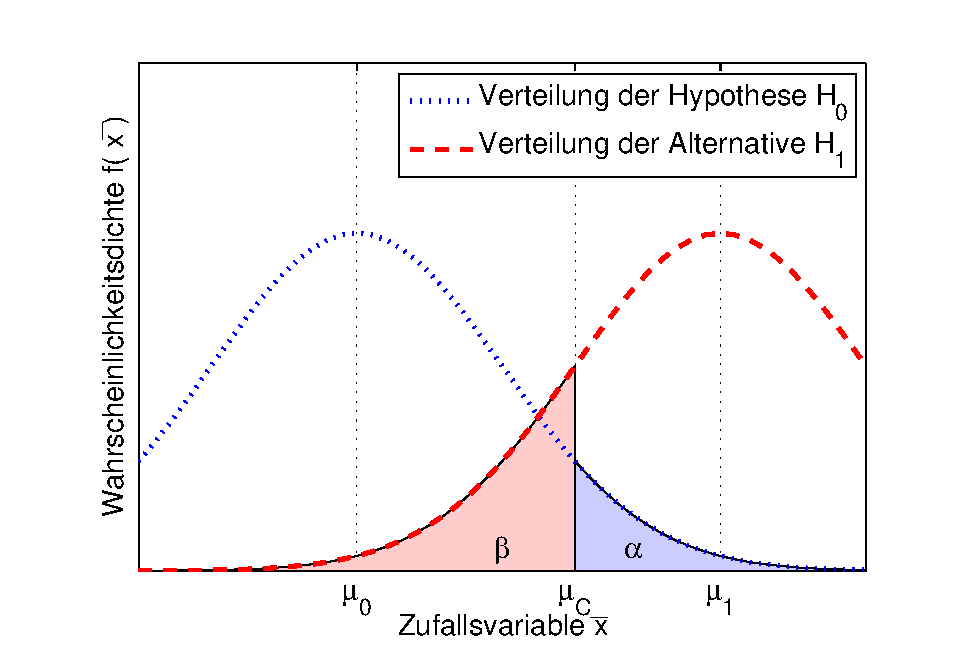
\includegraphics[width=0.5\textwidth]{Kapitel6/Bilder/image9}}
  \caption{Darstellung des Fehlers erster und zweiter Art beim Hypothesentest}
  \label{fig:HypothesentestFehler}
\end{figure}

\clearpage

{\fontfamily{phv}\selectfont
\noindent\textbf{Fehler erster Art}}\smallskip

\noindent Beim Fehler erster Art wird die Nullhypothese verworfen, obwohl sie richtig ist. Die Wahrscheinlichkeit, einen solchen Fehler zu begehen, entspricht der Irrtumswahrscheinlichkeit $\alpha$, die auch als Signifikanzniveau des Tests bezeichnet wird. Ein solcher Fehler wird begangen, wenn die Hypothese richtig ist und der berechnete Stichprobenwert $\overline{\mathrm{x}}$ trotzdem einen Wert annimmt, der oberhalb der kritischen Grenze µ$_{C}$ liegt. In diesem Fall gilt die bedingte Wahrscheinlichkeit

\begin{equation}\label{eq:sixfiftyseven}
P\left(\bar{x}>\mu _{C} |\mu =\mu _{0} \right)=\alpha
\end{equation}

\noindent In dem einf\"{u}hrenden Beispiel zur Prozesskontrolle ist ein Fehler erster Art, dass der Stichprobenmittelwert $\overline{\mathrm{x}}$ den Grenzwert µ$_{C2}$ \"{u}berschreitet, obwohl die Grundgesamtheit den richtigen Mittelwert µ$_{0}$ besitzt.\bigskip

{\fontfamily{phv}\selectfont
\noindent\textbf{Fehler zweiter Art}}\smallskip

\noindent Beim Fehler zweiter Art wird die Nullhypothese angenommen, obwohl diese falsch ist. Die zugeh\"{o}rige Wahrscheinlichkeit wird mit $\beta$ bezeichnet. Ein Fehler zweiter Art wird begangen, wenn die Nullhypothese falsch ist, der berechnete Stichprobenwert aber dennoch einen Wert annimmt, der unterhalb der kritischen Grenze µ$_{C}$ liegt. In diesem Fall gilt

\begin{equation}\label{eq:sixfiftyeight}
P\left(\bar{x}\le \mu _{C} |\mu =\mu _{1} \right)=\beta
\end{equation}

\noindent Der Wert (1 - $\beta$) ist die Wahrscheinlichkeit, einen Fehler zweiter Art zu vermeiden. Der Wert wird als G\"{u}te des Hypothesentests bezeichnet. \bigskip

{\fontfamily{phv}\selectfont
\noindent\textbf{Diskussion von Fehlern erster und zweiter Art}}\smallskip

\noindent Tabelle \ref{tab:sixfour} stellt die Situation von Annahme und Ablehnung einer Nullhypothese beim Hypothesentest und die damit verbundenen Fehler tabellarisch zusammen.

\begin{table}[H]
\setlength{\arrayrulewidth}{.1em}
\caption{\"{U}bersicht \"{u}ber richtige und falsche Entscheidungen beim Hypothesentest mit der entsprechenden Wahrscheinlichkeitsangabe}
\setlength{\fboxsep}{0pt}%
\colorbox{lightgray}{%
\arrayrulecolor{white}%
\begin{tabular}{| wc{1cm} | wc{1cm} | wc{7cm} | wc{7cm} }
\hline\xrowht{20pt}

\multirow{2}{*}{ } &  \multicolumn{3}{c}{\fontfamily{phv}\selectfont\textbf{Unbekannte Wirklichkeit}} \\ \xrowht{15pt}
& & {\fontfamily{phv}\selectfont\textbf{µ = µ$_{0}$}} & 
{\fontfamily{phv}\selectfont\textbf{µ = µ$_{1}$}} \\ \hline \xrowht{20pt}

\multirow{8}{*}{\fontfamily{phv}\selectfont\textbf{\begin{turn}{90}Angenommen\end{turn}}} & \multirow{3}{*}{\fontfamily{phv}\selectfont\textbf{\begin{turn}{90}µ = µ$_{0}$\end{turn}}} &
richtige Entscheidung & Fehler 2. Art\\\xrowht{20pt}

& & $p= 1 - \alpha$ & 
$p=\beta$ \\ \cline{2-4}\xrowht{20pt} 

& \multirow{3}{*}{\fontfamily{phv}\selectfont\textbf{\begin{turn}{90}µ = µ$_{1}$\end{turn}}} & Fehler 1. Art & richtige Entscheidung\\\xrowht{20pt}
& & $p= \alpha$ & $p=1 - \beta$ \\ \hline 

\end{tabular}%
}
\label{tab:sixfour}
\end{table}

\noindent Die Wahl des Parameters µ$_{C}$ bestimmt die Wahrscheinlichkeit der Fehlentscheidung. Der Parameter µ$_{C}$ sollte daher so gew\"{a}hlt werden, dass die Fehlerwahrscheinlichkeiten $\alpha$ und $\beta$ m\"{o}glichst klein werden. Bild \ref{fig:HypothesentestFehler} zeigt, dass diese Forderungen sich gegenseitig widersprechen. Um $\alpha$ zu minimieren, muss die kritische Grenze µ$_{C}$ nach rechts verschoben werden. Dann wird aber die Fehlerwahrscheinlichkeit $\beta$ gr\"{o}{\ss}er. Bei der praktischen Durchf\"{u}hrung von Hypothesentests wird zun\"{a}chst das Signifikanzniveau $\alpha$ festgelegt. Daraus ergibt sich die Grenze des Annahmebereiches µ$_{C}$ und mit dem Parameter µ$_{C}$ wird die Fehlerwahrscheinlichkeit $\beta$ des Fehlers zweiter Art berechnet.\newline

\noindent Die Annahme einer Hypothese ist stets von der vorliegenden Stichprobe und dem gew\"{a}hlten Signifikanzniveau $\alpha$ abh\"{a}ngig. Aus der Annahme einer Hypothese auf Basis eines Hypothesentests folgt daher nicht, dass die Hypothese die einzig m\"{o}gliche ist. Ein Hypothesentest sagt lediglich aus, ob auf Basis der vorliegenden Stichprobe und dem gew\"{a}hlten Signifikanzniveau $\alpha$ eine Hypothese aufrechterhalten werden kann oder verworfen werden muss. Oftmals ist auch die Fehlerwahrscheinlichkeit $\beta$ des Hypothesentests nicht bekannt, sodass weitere Bewertungen der Entscheidung nicht m\"{o}glich sind. Das Risiko erster Art kann dann zwar klein gew\"{a}hlt werden, dadurch steigt jedoch das Risiko zweiter Art. 

\subsubsection{G\"{u}tefunktion eines Hypothesentests}

\noindent Die G\"{u}tefunktion eines Hypothesentests erlaubt, Aussagen \"{u}ber die Qualit\"{a}t des statistischen Tests zu machen. Sie wird deshalb zum Vergleich unterschiedlicher Tests zu einem Testproblem herangezogen. Falls mehrere konkurrierende Tests existieren, wird der Test ausgew\"{a}hlt, der bei gleichem Stichprobenumfang die gr\"{o}{\ss}te G\"{u}te beziehungsweise die gr\"{o}{\ss}te Trennsch\"{a}rfe besitzt. F\"{u}r die bekannten Alternativhypothesen

\begin{equation}\label{eq:sixfiftynine}
\mu _{1} >\mu _ 0
\end{equation}
\begin{equation}\label{eq:sixsixty}
\mu _{1} <\mu _ 0
\end{equation}
\begin{equation}\label{eq:sixsixtyone}
\mu _{1} \ne \mu _ 0
\end{equation}

\noindent wird die G\"{u}te (1 - $\beta$) als Funktion der alternativen Pr\"{u}fgr\"{o}{\ss}e µ$_{1}$ beschrieben. Es wird deshalb nicht mehr von der G\"{u}te, sondern von einer G\"{u}tefunktion gesprochen.\newline

\noindent Die G\"{u}tefunktion eines Hypothesentests wird an einem Beispiel mit einer normalverteilten Grundgesamtheit und bekannter Varianz $\sigma^{2}$= 9 diskutiert. Unter Verwendung einer Stichprobe mit einem Umfang von N = 10 Messwerten und dem Stichprobenmittelwert $\overline{\mathrm{x}}$ soll die Nullhypothese µ = µ$_{0}$ = 24 gegen die drei Varianten der Alternativhypothese aus Gleichungen \eqref{eq:sixfiftynine} - \eqref{eq:sixsixtyone} getestet werden.\newline

\noindent F\"{u}r die weiteren Betrachtungen wird ein Signifikanzniveau von $\alpha$ = 5 \% gew\"{a}hlt. Trifft die Nullhypothese zu, ist der Mittelwert der Grundgesamtheit normalverteilt mit dem Mittelwert µ$_{0}$ = 24 und der Standardabweichung 

\begin{equation}\label{eq:sixsixtytwo}
\sigma _{\bar{x}} =\dfrac{\sigma}{\sqrt{N}} =\sqrt{0.9}
\end{equation}

\noindent F\"{u}r die Berechnung des kritischen Wertes µ$_{C}$ wird die standardnormalverteilte Pr\"{u}fgr\"{o}{\ss}e 

\begin{equation}\label{eq:sixsixtythree}
z=\dfrac{\bar{x}-\mu _{0}}{\sigma _{\bar{x}}} =\dfrac{\bar{x}-\mu _{0}}{\sigma /\sqrt{N}} =\dfrac{\bar{x}-24}{\sqrt{0.9}}
\end{equation}

\noindent herangezogen. Mit dieser Verteilung kann der Annahmebereich der Nullhypothese berechnet werden. Die unterschiedlichen Alternativhypothesen werden im Folgenden einzeln hinsichtlich ihrer Annahme- und Verwerfungsbereiche sowie der G\"{u}te des Tests diskutiert.

\clearpage

{\fontfamily{phv}\selectfont
\noindent\textbf{Alternativhypothese µ$_{1} >$ µ$_{0}$}}\smallskip

\noindent Zun\"{a}chst wird die Alternativhypothese µ${}_{1}  \boldsymbol > $ µ${}_{0}$ untersucht. Die Berechnung des Annahmebereiches erfolgt in diesem Fall durch die Wahrscheinlichkeit 

\begin{equation}\label{eq:sixsixtyfour}
P\left(\bar{x}<\mu _{C} |\mu =\mu _{0} \right)=P\left(\bar{x}<\mu _{0} +\dfrac{c\cdot \sigma }{\sqrt{N} } |\mu =\mu _{0} \right)=\gamma =1-\alpha
\end{equation}

\noindent Die Grenze c ergibt sich aus der inversen Standardnormalverteilung zu c = 1.6449. Damit folgt die Grenze des Annahmebereiches mit der Nullhypothese µ$_{0}$ = 24 zu

\begin{equation}\label{eq:sixsixtyfive}
\bar{x}<\mu _{0} +\dfrac{c\cdot \sigma }{\sqrt{N} } =25.56
\end{equation}

Liegt der Stichprobenmittelwert unterhalb der kritischen Grenze µ$_{C}$ = 25.56 wird die Nullhypothese angenommen, andernfalls wird die Nullhypothese abgelehnt. Nach Festlegung des Grenzwertes µ$_{C}$ kann die G\"{u}te des Hypothesentests mit der Alternativhypothese µ$_{1} > $ µ$_{0}$ berechnet werden zu

\begin{equation}\label{eq:sixsixtysix}
1-\beta \left(\mu _{1} \right)=P\left(\bar{x}>\mu _{C} |\mu =\mu _{1} \right)=1-P\left(\bar{x}<\mu _{C} |\mu =\mu _{1} \right)
\end{equation}

\noindent Wegen der Standardisierung der Zufallsvariable $\bar{x}$ kann die G\"{u}tefunktion mit der Standardnormalverteilung ausgedr\"{u}ckt werden.

\begin{equation}\label{eq:sixsixtyseven}
1-\beta \left(\mu _{1} \right)=1-P\left(\bar{x}<\mu _{C} |\mu =\mu _{1} \right)=1-F\left(\dfrac{\mu _{C} -\mu _{1} }{\sigma _{\bar{x}} } \right)=1-F\left(\dfrac{25.56-\mu _{1} }{\sqrt{0.9} } \right)
\end{equation}

\noindent Die G\"{u}te ist davon abh\"{a}ngig, wie gro{\ss} der Alternativmittelwert µ$_{1}$ ist. Die entsprechende G\"{u}tefunktion ist in Bild \ref{fig:HypothesentestFehler1} dargestellt.

\noindent 
\begin{figure}[H]
  \centerline{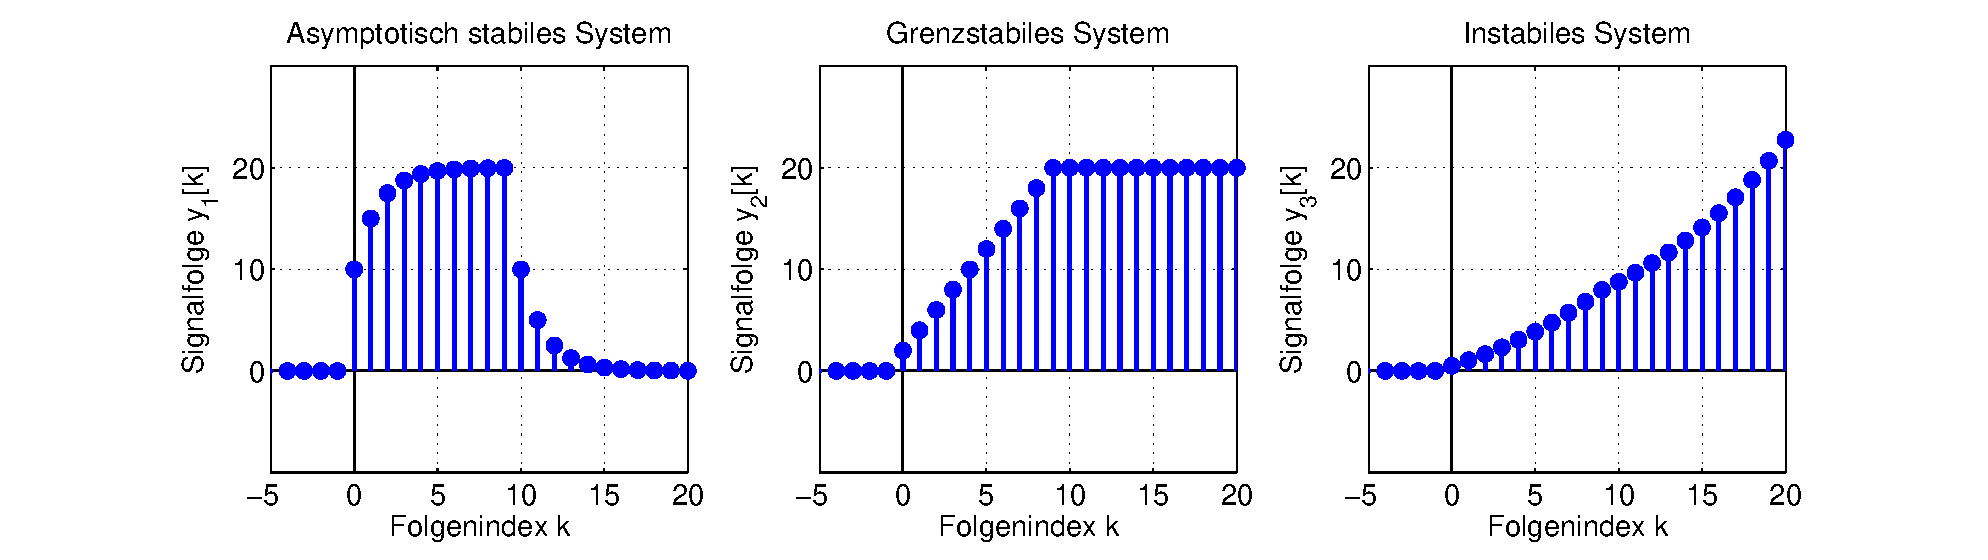
\includegraphics[width=0.5\textwidth]{Kapitel6/Bilder/image10}}
  \caption{Darstellung der G\"{u}tefunktion f\"{u}r die Alternativhypothese µ$_{1} >$ µ$_{0}$}
  \label{fig:HypothesentestFehler1}
\end{figure}

\noindent Je gr\"{o}{\ss}er der Wert µ$_{1}$ ist, desto sicherer ist die Aussage, dass die Mittelwerte voneinander abweichen. F\"{u}r µ$_{1}$ = µ$_{0}$ hat die G\"{u}te den Wert des Signifikanzniveaus $\alpha$. Angenommen der wahre Mittelwert liegt bei µ$_{1}$ = 26, dann ist die G\"{u}te dieses Tests ca. 70 \%. Ein Mittelwert µ$_{1}$ = 26 wird demnach nur mit einer Wahrscheinlichkeit von 70 \% als Fehler erkannt.

\clearpage

{\fontfamily{phv}\selectfont
\noindent\textbf{Alternativhypothese µ$_{1} <$ µ$_{0}$}}\smallskip

\noindent F\"{u}r die Alternativhypothese µ$_{1} <$ µ$_{0}$wird der Annahmebereich mit der Wahrscheinlichkeit

\begin{equation}\label{eq:sixsixtyeight}
P\left(\bar{x}>\mu _{C} |\mu =\mu _{0} \right)=P\left(\bar{x}>\mu _{0} +\dfrac{c\cdot \sigma }{\sqrt{N} } |\mu =\mu _{0} \right)=\gamma =1-\alpha
\end{equation}

\noindent berechnet. Die Grenze c ergibt sich dabei aus der inversen Standardnormalverteilung zu c = - 1.6449. Mit diesem Wert berechnet sich der Annahmebereich bei der Alternativhypothese µ$_{1} <$ µ$_{0}$ mit der Nullhypothese µ$_{0}$ = 24 zu

\begin{equation}\label{eq:sixsixtynine}
\bar{x}>\mu _{0} +\dfrac{c\cdot \sigma }{\sqrt{N} } =22.44
\end{equation}

\noindent Liegt der Stichprobenmittelwert oberhalb der kritischen Grenze µ$_{C}$ = 22.44, wird die Nullhypothese angenommen, andernfalls wird die Nullhypothese abgelehnt.\newline

\noindent Nach Festlegung des Grenzwertes µ$_{C}$ kann die G\"{u}te des Hypothesentests mit der Alternativhypothese µ$_{1} <$ µ$_{0}$ berechnet werden zu

\begin{equation}\label{eq:sixseventy}
1-\beta (\mu _{1})=P\left(\bar{x}<\mu _{C} |\mu =\mu _{1} \right)=F\left(\dfrac{\mu _{C} -\mu _{1}}{\sigma _{\bar{x}}} \right)=F\left(\dfrac{22.44-\mu _{1}}{\sqrt{0.9} } \right)
\end{equation}

\noindent Wieder ist die G\"{u}te davon abh\"{a}ngig, wie gro{\ss} der Alternativmittelwert µ$_{1}$ ist. Die G\"{u}tefunktion ist in Bild \ref{fig:HypothesentestFehler2} dargestellt.

\noindent 
\begin{figure}[H]
  \centerline{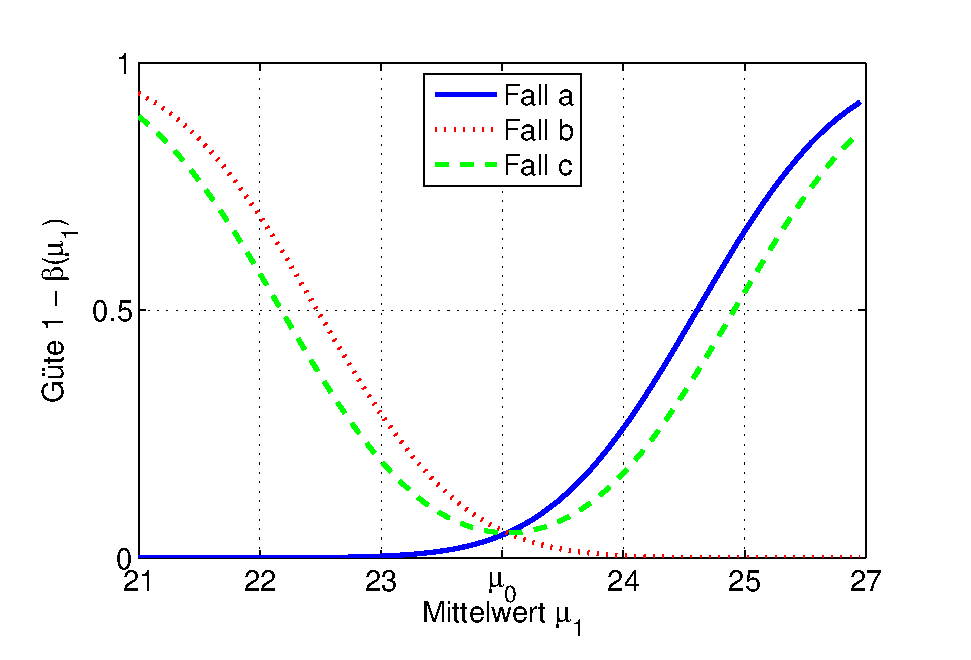
\includegraphics[width=0.5\textwidth]{Kapitel6/Bilder/image11}}
  \caption{Darstellung der G\"{u}tefunktion f\"{u}r die Alternativhypothese µ$_{1} <$ µ$_{0}$}
  \label{fig:HypothesentestFehler2}
\end{figure}

\noindent Je kleiner der Wert µ$_{1}$ ist, desto sicherer ist die Aussage, dass die Mittelwerte voneinander abweichen. F\"{u}r µ$_{1}$ = µ$_{0}$ hat die G\"{u}te den Wert des Signifikanzniveaus $\alpha$. Angenommen der wahre Mittelwert liegt bei µ$_{1}$ = 22, dann ist die G\"{u}te dieses Tests ca. 70 \%. Ein Mittelwert µ$_{1}$ = 22 wird demnach nur mit einer Wahrscheinlichkeit von ca. 70 \% als Fehler erkannt.

\clearpage

{\fontfamily{phv}\selectfont
\noindent\textbf{Alternativhypothese µ$_{1} \neq$ µ$_{0}$}}\smallskip

\noindent Die Alternativhypothese µ$_{1} \neq$ µ$_{0}$ f\"{u}hrt zu einem zweiseitigen Verwerfungsbereich der Nullhypothese. Der Annahmebereich ergibt sich aus der Definition der Annahmewahrscheinlichkeit

\begin{equation}\label{eq:sixseventyone}
P\left(\mu _{C1} <\bar{x}\le \mu _{C2} |\mu =\mu _{0} \right)=P\left(\mu _{0} +\dfrac{c_{1} \cdot \sigma }{\sqrt{N} } <\bar{x}\le \mu _{0} +\dfrac{c_{2} \cdot \sigma }{\sqrt{N} } |\mu =\mu _{0} \right)=\gamma =1-\alpha
\end{equation}

\noindent Damit ergibt sich der Annahmebereich in diesem Beispiel zu

\begin{equation}\label{eq:sixseventytwo}
22.14=\mu _{0} +\dfrac{c_{1} \cdot \sigma}{\sqrt{N}} <\bar{x}\le \mu _{0} +\dfrac{c_{2} \cdot \sigma}{\sqrt{N}} =25.86
\end{equation}

\noindent Liegt der Stichprobenmittelwert innerhalb der Grenzen µ$_{C1}$ = 22.14 und µ$_{C2}$ = 25.86 wird die Nullhypothese angenommen, andernfalls wird die Nullhypothese abgelehnt.\noindent

\noindent Bei der Berechnung der G\"{u}te m\"{u}ssen bei der Alternativhypothese µ$_{1} \neq$ µ$_{0}$ zwei Bereiche ber\"{u}cksichtigt werden. Damit ergibt sich bei einem alternativen Mittelwert µ$_{1}$ die G\"{u}tefunktion

\begin{equation}\label{eq:sixseventythree}
\begin{split}
1-\beta \left(\mu _{1} \right) & = P\left(\bar{x}<\mu _{C1} |\mu =\mu _{1} \right)+P\left(\bar{x}>\mu _{C2} |\mu =\mu _{1} \right) \\ 
& = P\left(\bar{x}<\mu _{C1} |\mu =\mu _{1} \right)+1-P\left(\bar{x}<\mu _{C2} |\mu =\mu _{1} \right)    
\end{split}
\end{equation}

\noindent Damit berechnet sich die G\"{u}tefunktion f\"{u}r das vorliegende Beispiel durch die Standardnormalverteilung aus 

\begin{equation}\label{eq:sixseventyfour}
1-\beta \left(\mu _{1} \right)=1+F\left(\dfrac{\mu _{C1} -\mu _{1} }{\sigma /\sqrt{N} } \right)-F\left(\dfrac{\mu _{C2} -\mu _{1} }{\sigma /\sqrt{N} } \right)=1+F\left(\dfrac{22.14-\mu _{1} }{\sqrt{0.9} } \right)-F\left(\dfrac{25.86-\mu _{1} }{\sqrt{0.9} } \right)
\end{equation}

\noindent Bild \ref{fig:HypothesentestFehler3} stellt die G\"{u}te des Hypothesentests mit der Alternativhypothese µ$_{1} \neq$ µ$_{0}$ als Funktion des alternativen Mittelwertes µ$_{1}$ dar. 

\noindent 
\begin{figure}[H]
  \centerline{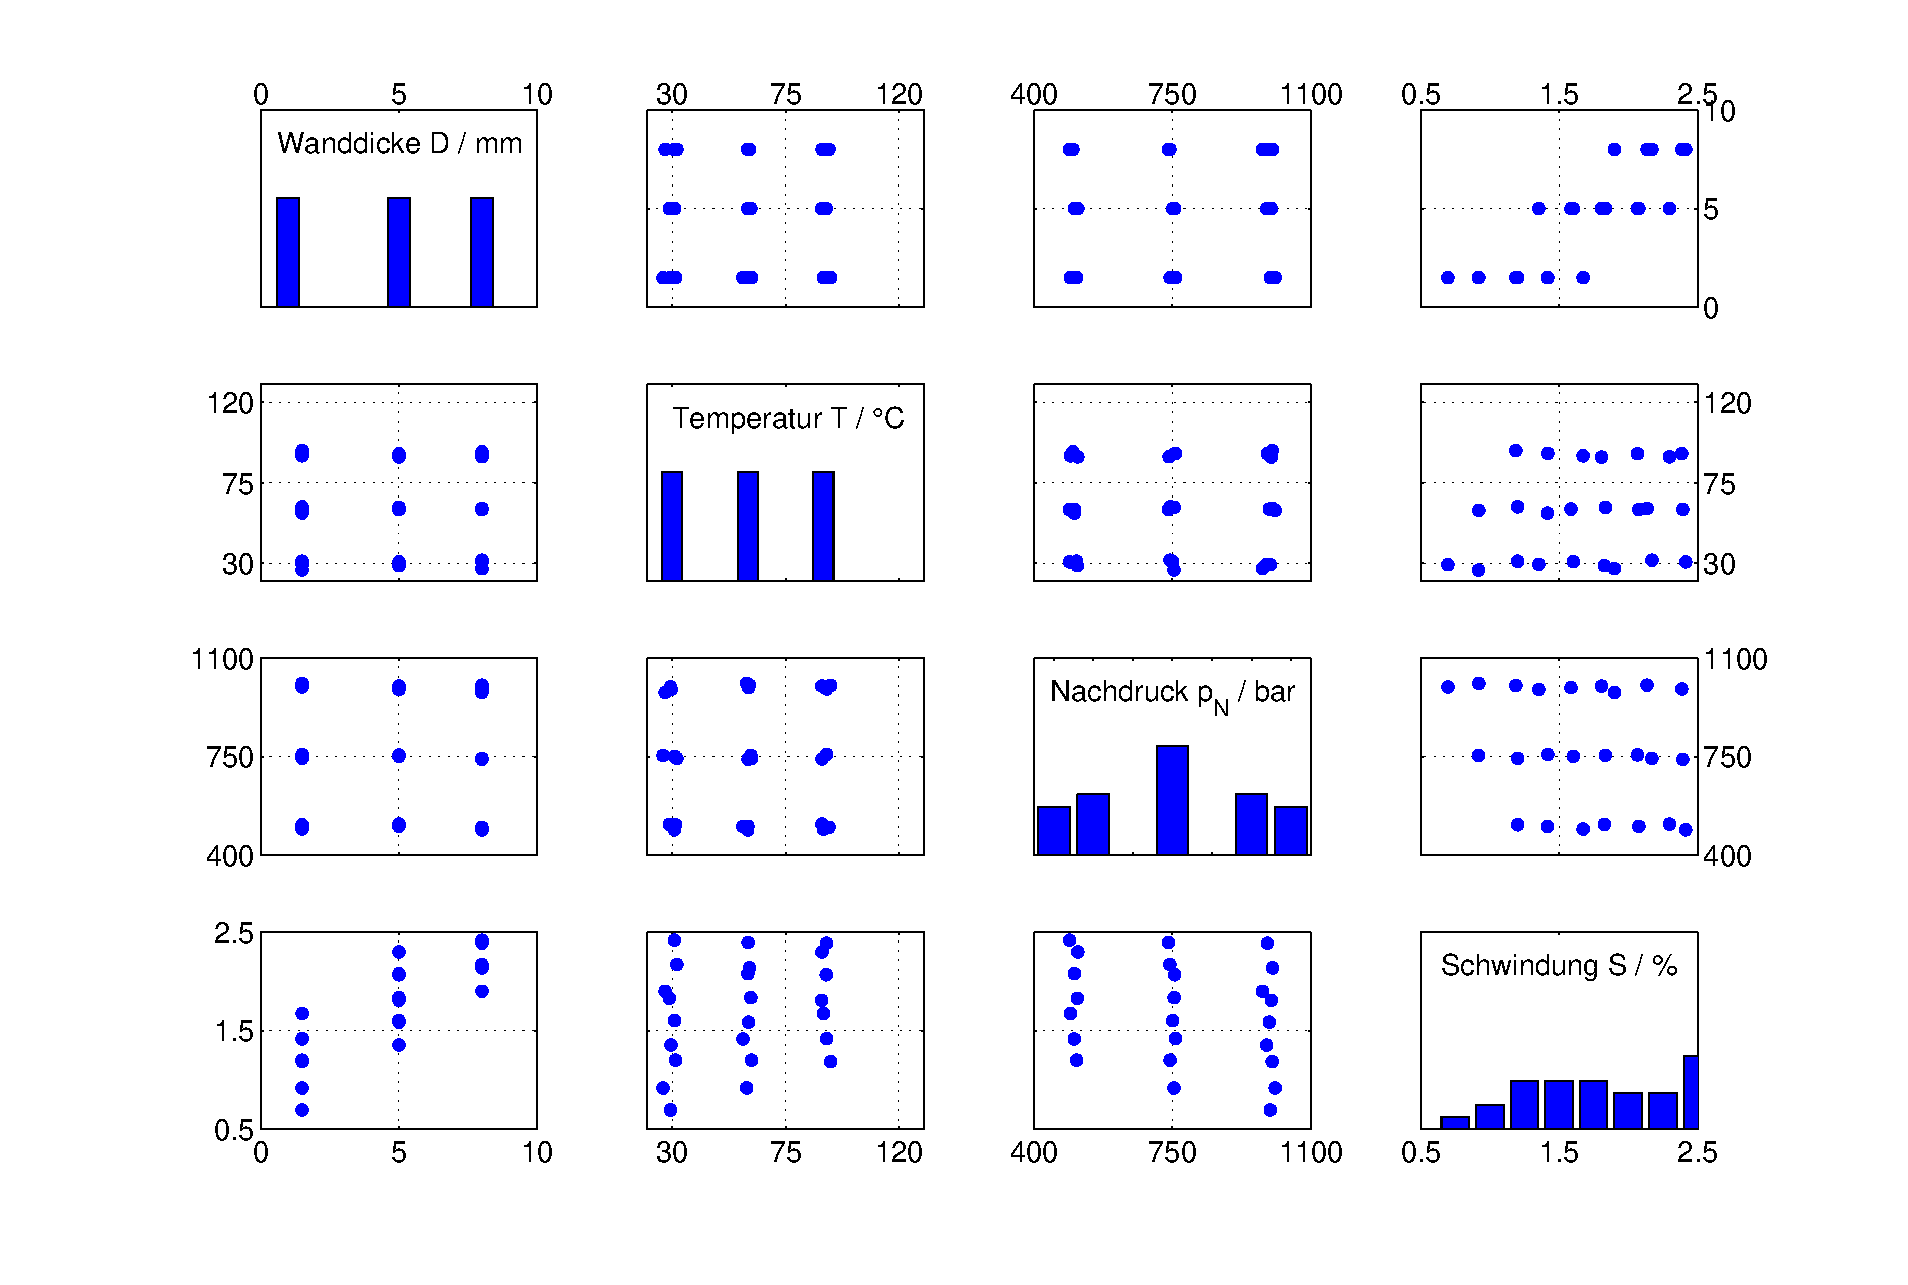
\includegraphics[width=0.5\textwidth]{Kapitel6/Bilder/image12}}
  \caption{Darstellung der G\"{u}tefunktion f\"{u}r die Alternativhypothese µ$_{1} \neq$ µ$_{0}$}
  \label{fig:HypothesentestFehler3}
\end{figure}

\noindent Je weiter der Wert µ$_{1}$ von dem Wert µ$_{0}$ abweicht, desto sicherer ist erwartungsgem\"{a}{\ss} die Aussage, dass die Mittelwerte voneinander abweichen. F\"{u}r µ$_{1}$ = µ$_{0}$ besitzt die G\"{u}te den Wert des Signifikanzniveaus $\alpha$. Angenommen der wahre Mittelwert liegt bei µ$_{1}$ = 26, dann ist die G\"{u}te dieses Tests ca. 55 \%. Ein Mittelwert µ$_{1}$ = 26 wird nur mit einer Wahrscheinlichkeit von ca. 55 \% als Fehler erkannt.\newline

\noindent W\"{u}rde der Test mit einem gr\"{o}{\ss}eren Stichprobenumfang von N = 100 durchgef\"{u}hrt, w\"{u}rde sich die Varianz des Mittelwertes verkleinern und die kritischen Grenzen erg\"{a}ben sich zu µ$_{C1}$ = 23.41 und µ$_{C2}$ = 24.59. Bild \ref{fig:HypothesentestFehler4} verdeutlicht f\"{u}r die Alternativhypothese µ$_{1}$ $\neq$ µ${}_{0}$, dass mit h\"{o}herem Stichprobenumfang die G\"{u}tefunktion des Hypothesentests einen steileren Verlauf bekommt, also eine gr\"{o}{\ss}ere Trennsch\"{a}rfe besitzt als bei kleinerem Stichprobenumfang. 

\noindent 
\begin{figure}[H]
  \centerline{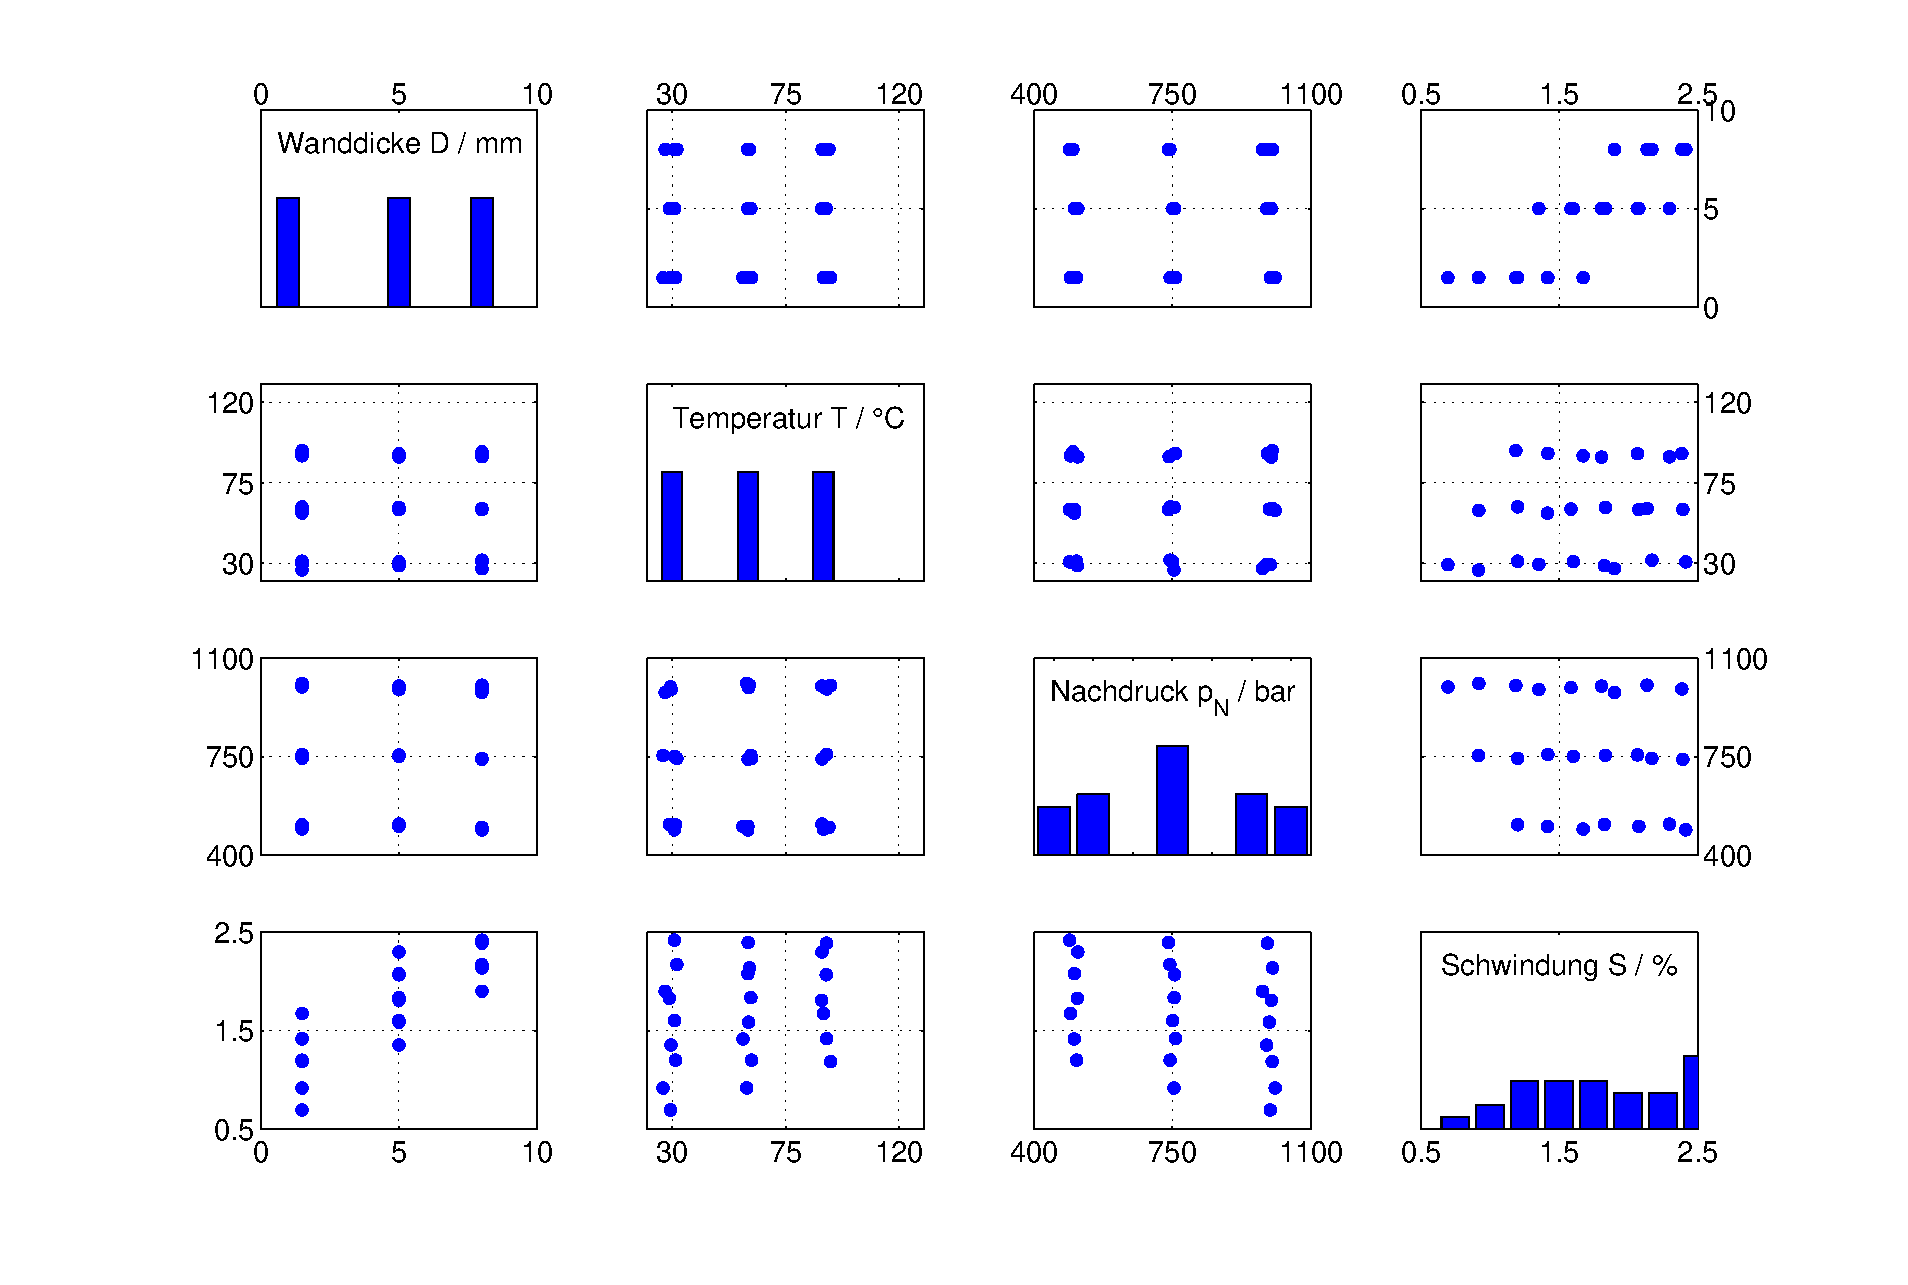
\includegraphics[width=0.5\textwidth]{Kapitel6/Bilder/image12}}
  \caption{Darstellung der G\"{u}tefunktion f\"{u}r die Alternativhypothese µ$_{1} \neq$ µ$_{0}$ mit unterschiedlichen Stichprobenumf\"{a}ngen}
  \label{fig:HypothesentestFehler4}
\end{figure}

\noindent Wird der Stichprobenumfang erh\"{o}ht, wird ein wahrer Mittelwert von µ$_{1}$ = 26 mit einer G\"{u}te von praktisch 100 \% erkannt. \newline

\noindent Allerdings muss der Stichprobenumfang in der Praxis aus Kostengr\"{u}nden so klein wie m\"{o}glich gehalten werden. Interessiert zum Beispiel eine Abweichung von $\pm$ 2 Einheiten, so ist f\"{u}r dieses Beispiel eine Stichprobe vom Umfang von N = 10 Werten zu gering, denn f\"{u}r die Werte µ = 22 und 26 betr\"{a}gt das Risiko eines Fehlers zweiter Art noch fast 50 \%. Mit einem Stichprobenumfang von N = 100 Werten reicht die Aussagesicherheit sicher aus, die Wahrscheinlichkeit f\"{u}r einen Fehler zweiter Art betr\"{a}gt f\"{u}r die Werte µ = 22 und 26 weniger als 1 ppm. Realistisch ist ein Stichprobenumfang zwischen diesen Werten. In Abschnitt 6.4.3 wird die Absch\"{a}tzung des erforderlichen Stichprobenumfangs f\"{u}r die Erkennung einer Abweichung von Mittelwerten diskutiert.\newline

\noindent Die Eigenschaften der G\"{u}tefunktion lassen sich wie folgt zusammenfassen:

\begin{itemize}
    \item Mit sinkendem Signifikanzniveau $\alpha$ sinkt die G\"{u}te des Tests und die Wahrscheinlichkeit f\"{u}r den Fehler zweiter Art steigt an.
    \item  Die G\"{u}te wird mit wachsendem Abstand der Parameter µ$_{0}$ und µ$_{1}$ gr\"{o}{\ss}er.
    \item  Mit wachsendem Stichprobenumfang N wird die Trennsch\"{a}rfe eines Hypothesentests gr\"{o}{\ss}er.
\end{itemize}

{\fontfamily{phv}\selectfont
\noindent\textbf{Absch\"{a}tzung des notwendigen Stichprobenumfang}}\smallskip

\noindent Auf Basis des Signifikanzniveaus $\alpha$ und der G\"{u}tefunktion (1 - $\beta$) kann der Stichprobenumfang abgesch\"{a}tzt werden, der f\"{u}r eine Unterscheidung von zwei Mittelwerten mit der Differenz $\Delta\mu$ mit einer definierten G\"{u}te notwendig ist. Ausgangspunkt f\"{u}r die hier dargestellte Absch\"{a}tzung ist aus Gr\"{u}nden der \"{U}bersichtlichkeit eine normalverteilte Grundgesamtheit mit der bekannten Standardabweichung $\sigma$. Die zu pr\"{u}fende Nullhypothese ist, dass die Grundgesamtheit den Mittelwert µ$_{0}$ aufweist. Als Alternativhypothese wird ein Mittelwert µ$_{1} >$ µ$_{0}$ gepr\"{u}ft. Die Nullhypothese wird mit dem Signifikanzniveau $\alpha$ gepr\"{u}ft. Damit ergibt sich f\"{u}r die Annahme des Hypothesentests eine Grenze µ$_{C}$ f\"{u}r die Annahme mit der Bedingung

\begin{equation}\label{eq:sixseventyfive}
P\left(\bar{x}<\mu _{C} |\mu =\mu _{0} \right)=P\left(\bar{x}<\mu _{0} +\dfrac{c\cdot \sigma }{\sqrt{N} } |\mu =\mu _{0} \right)=F\left(\dfrac{\mu _{C} -\mu _{0} }{\sigma /\sqrt{N}} \right)=\gamma =1-\alpha
\end{equation}

\noindent Durch Aufl\"{o}sen der Gleichung \eqref{eq:sixseventyfive} ergibt sich mit der inversen Standardnormalverteilung die Grenze des Annahmebereich µ$_{C}$ zu

\begin{equation}\label{eq:sixseventysix}
\mu _{C} =F^{-1} \left(1-\alpha \right)\cdot \dfrac{\sigma }{\sqrt{N}} +\mu _{0}
\end{equation}

\noindent Die G\"{u}tefunktion ergibt sich unter Annahme der Alternativhypothese µ$_{1} >$ µ$_{0}$ zu

\begin{equation}\label{eq:sixseventyseven}
1-\beta \left(\mu _{1} \right)=P\left(\bar{x}>\mu _{C} |\mu =\mu _{1} \right)=1-P\left(\bar{x}<\mu _{C} |\mu =\mu _{1} \right)=1-F\left(\dfrac{\mu _{C} -\mu _{1} }{\sigma /\sqrt{N} } \right)
\end{equation}

\noindent Durch Umformen von Gleichung \eqref{eq:sixseventyseven} ergibt sich ein weiterer Ausdruck f\"{u}r die Grenze des Annahmebereichs µ$_{C}$ zu

\begin{equation}\label{eq:sixseventyeight}
\mu _{C} =F^{-1} \left(\beta \left(\mu _{1} \right)\right)\cdot \dfrac{\sigma }{\sqrt{N} } +\mu _{1}
\end{equation}

\noindent Um eine Gleichung f\"{u}r die Absch\"{a}tzung des Stichprobenumfangs zu erhalten, werden Gleichung \eqref{eq:sixseventysix} und Gleichung \eqref{eq:sixseventyeight} zusammengef\"{u}hrt

\begin{equation}\label{eq:sixseventynine}
\mu _{C} =F^{-1} \left(1-\alpha \right)\cdot \dfrac{\sigma }{\sqrt{N} } +\mu _{0} =F^{-1} \left(\beta \left(\mu _{1} \right)\right)\cdot \dfrac{\sigma }{\sqrt{N} } +\mu _{1}
\end{equation}

\noindent und nach dem Stichprobenumfang N aufgel\"{o}st

\begin{equation}\label{eq:sixeighty}
N=\left(\dfrac{\sigma }{\mu _{1} -\mu _{0} } \right)^{2} \cdot \left(F^{-1} (1-\alpha)-F^{-1} \left(\beta \left(\mu _{1} \right)\right)\right)^{2} =\left(\dfrac{\sigma }{\Delta \mu } \right)^{2} \cdot \left(F^{-1} \left(1-\alpha \right)-F^{-1} \left(\beta (\mu _{1} )\right)\right)^{2}
\end{equation}

\noindent Der Stichprobenumfang steigt erwartungsgem\"{a}{\ss} mit wachsendem Verh\"{a}ltnis von Standardabweichung $\sigma$ zum Abstand $\Delta\mu$ der zu unterscheidenden Mittelwerte an. F\"{u}r ein typisches Signifikanzniveau von $\alpha$ = 5 \% und eine G\"{u}te von 1 - $\beta$ = 90 \% ergibt sich

\begin{equation}\label{eq:sixeightyone}
N=\left(\dfrac{\sigma }{\Delta \mu } \right)^{2} \cdot 8.56
\end{equation}

\noindent Die hier durchgef\"{u}hrte Herleitung gilt unter der Annahme einer einseitigen Alternative und bekannter Standardabweichung $\sigma$. Analog kann auch f\"{u}r eine zweiseitige Alternativhypothese µ$_{1} \neq$ µ$_{0}$ und eine unbekannte Standardabweichung $\sigma$ vorgegangen werden. Beide \"{A}nderungen f\"{u}hren zu einer Vergr\"{o}{\ss}erung des notwendigen Stichprobenumfangs. In der Literatur wird deshalb f\"{u}r den Stichprobenumfang die Absch\"{a}tzung

\begin{equation}\label{eq:sixeightytwo}
N=\left(\dfrac{\sigma }{\Delta \mu } \right)^{2} \cdot 30
\end{equation}

\noindent angegeben. 

\clearpage

\subsection{Hypothesentests f\"{u}r die Parameter einer Normalverteilung}

\noindent In den folgenden Abschnitten werden verschiedenen Hypothesentests f\"{u}r die Parameter einer Normalverteilung vorgestellt. Dabei wird von einem zweiseitig begrenzten Annahmebereich ausgegangen. Bei Hypothesentests f\"{u}r einseitig begrenzte Annahmebereiche muss die Grenze des Annahmebereichs µ$_{C}$ entsprechend der Alternativhypothese angepasst werden. Dieses Vorgehen wird anhand einiger Beispiele dargestellt.

\subsubsection{Test auf Mittelwert \texorpdfstring{$\mu_{0}$}{Lg} bei bekannter Varianz (Ein-Stichproben-z-Test)}

\noindent Der Test auf einen bestimmten Mittelwert $\mu_{0}$ bei bekannter Varianz wird bereits als einf\"{u}hrendes Beispiel in Abschnitt 6.1 herangezogen. Der Hypothesentest arbeitet mit den Hypothesen
\begin{itemize}
    \item Nullhypothese $H_{0} : \mu = \mu_{0}$
    \item Alternativhypothese $H_{1} : \mu \neq \mu_{0}$
\end{itemize}

\noindent Dieser Test wird auch als Gau{\ss}- oder z-Test bezeichnet. Er wird bei einer zumindest n\"{a}herungsweise normalverteilten Stichprobe mit bekannter Varianz angewendet. Das Vorgehen kann in die folgenden Prozessschritte aufgeteilt werden:

\begin{table}[H]
\setlength{\arrayrulewidth}{.1em}
\caption{Vorgehen zum Hypothesentest f\"{u}r den Mittelwert einer Normalverteilung mit bekannter Varianz}
\setlength{\fboxsep}{0pt}%
\colorbox{lightgray}{%
\arrayrulecolor{white}%
\begin{tabular}{| wc{1cm} | wc{7.5cm} | wc{7.5cm}}
\xrowht{15pt}

\fontfamily{phv}\selectfont\textbf{Nr.} & 
\multicolumn{2}{c}{\fontfamily{phv}\selectfont\textbf{Prozessschritt}}\\ \hline \xrowht{20pt}

\fontfamily{phv}\selectfont{1} &
\multicolumn{2}{c}{\fontfamily{phv}\selectfont{Wahl eines Signifikanzniveaus $\alpha$}}\\ \hline \xrowht{10pt}

\multirow{4}{*}{\fontfamily{phv}\selectfont{2}} &
\multicolumn{2}{c}{\fontfamily{phv}\selectfont{Bestimmung der zugehörigen Parameter c$_{1}$ und c$_{2}$ aus der inversen}} \\ \xrowht{10pt}
& \multicolumn{2}{c}{\fontfamily{phv}\selectfont{Standardnormalverteilung}}  \\\xrowht{25pt}
& \multicolumn{2}{c}{\fontfamily{phv}\selectfont{$F(c_{1})=\dfrac{\alpha }{2} \qquad \qquad \qquad \qquad $  und  $\qquad \qquad \qquad \qquad F(c_{2} )=1-\dfrac{\alpha }{2}$}}  \\ \hline
\xrowht{20pt}

\multirow{3}{*}{\fontfamily{phv}\selectfont{3}} &
\multicolumn{2}{c}{\fontfamily{phv}\selectfont{Berechnung des Mittelwertes aus der Stichprobe}} \\ \xrowht{10pt}
& \multicolumn{2}{c}{\fontfamily{phv}\selectfont{$\bar{x}_{0} =\dfrac{1}{N} \cdot \left(x_{1} +x_{2} +...+x_{N} \right)=\dfrac{1}{N} \cdot \sum _{n=1}^{N}x_{n}  $}}  \\ \hline
\xrowht{20pt}

\multirow{4}{*}{\fontfamily{phv}\selectfont{4}}  &
\fontfamily{phv}\selectfont{Bestimmung des Konfidenzintervalls} & \fontfamily{phv}\selectfont{Berechnung des p-Wertes mit der} \\ 
& & \fontfamily{phv}\selectfont{Standardnormalverteilung} \\ \xrowht{20pt}
& \fontfamily{phv}\selectfont{$\mu _{C1} =\mu _{0} +\dfrac{c_{1} \cdot \sigma }{\sqrt{N} } <\bar{x}_{0} \le \mu _{0} +\dfrac{c_{2} \cdot \sigma }{\sqrt{N} } =\mu _{C2} $} & \fontfamily{phv}\selectfont{$p=F\left(\dfrac{\bar{x}_{0} -\mu _{0} }{\sigma /\sqrt{N} } \right)$} \\ \hline\xrowht{15pt}

\multirow{4}{*}{\fontfamily{phv}\selectfont{5}}  &
\fontfamily{phv}\selectfont{F\"{u}r $\nu_{C1}^{2} \leq \bar{x}_{0}^{2} <  \nu_{C2}^{2}$ wird die Hypothese} & \fontfamily{phv}\selectfont{ F\"{u}r $\alpha$/2 $\leq$ p $ < $ 1 - $\alpha$/2 wird die Hypothese  } \\ \xrowht{15pt}
& \fontfamily{phv}\selectfont{angenommen, f\"{u}r $\bar{x}_{0}^{2} \leq$ $\nu_{C1}^{2}$ oder $\bar{x}_{0}^{2} > \nu_{C2}^{2}$} & \fontfamily{phv}\selectfont{angenommen, f\"{u}r p $< \alpha$/2 und p $ \ge $ 1 -- $\alpha$/2 } \\ \xrowht{15pt}
&  \fontfamily{phv}\selectfont{wird die Hypothese verworfen} & \fontfamily{phv}\selectfont{wird die Hypothese verworfen } \\ \hline

\end{tabular}%
}\bigskip
\label{tab:sixfive}
\end{table}

\noindent F\"{u}r einseitige Testbedingungen m\"{u}ssen die Grenzen µ$_{C}$ entsprechend angepasst werden. Beispiele f\"{u}r den z-Test wurde bereits im einf\"{u}hrenden Beispiel zur Prozesskontrolle und in der Diskussion zu den verschiedenen Alternativhypothesen in Abschnitt 6.1 vorgestellt.

\clearpage

\subsubsection{Test auf eine Standardabweichung \texorpdfstring{$\sigma_{0}$}{Lg} (Ein-Stichproben-Chi-Quadrat-Test)}

\noindent Bei der Herleitung des Konfidenzbereichs der Varianz wird in Abschnitt 4.7.1 gezeigt, dass die Zufallsvariable

\begin{equation}\label{eq:sixeightythree}
\chi =\dfrac{s^{2}}{\sigma ^{2}} \cdot (N-1)
\end{equation}

\noindent eine Chi-Quadrat-Verteilung mit N - 1 Freiheitsgraden besitzt. Die Wahrscheinlichkeit $\gamma$, mit der die Variable $\chiup$ innerhalb des Intervalls c$_{1}$ {\dots} c$_{2}$ liegt, ist definiert als

\begin{equation}\label{eq:sixeightyfour}
\gamma =P\left(c_{1} <\chi \le c_{2} \right)=F(c_{2})-F(c_{1})
\end{equation}

\noindent Durch Einsetzen von Gleichung~\eqref{eq:sixeightythree} in die Definitionsgleichung der Wahrscheinlichkeit $\gamma$ ergibt sich ein Ausdruck f\"{u}r den Annahmebereich der Nullhypothese.

\begin{equation}\label{eq:sixeightyfive}
\gamma =P\left(c_{1} <\dfrac{s^{2} }{\sigma _{0}^{2} } \cdot \left(N-1\right)\le c_{2} \right)=P\left(\dfrac{c_{1} }{\left(N-1\right)} \cdot \sigma _{0}^{2} <s^{2} \le \dfrac{c_{2} }{\left(N-1\right)} \cdot \sigma _{0}^{2} \right)=P\left(\sigma _{C1}^{2} <s^{2} \le \cdot \sigma _{C2}^{2} \right)
\end{equation}

\noindent Liegt die vorliegende Stichprobenvarianz s$_{0}^{2}$ in dem definierten Intervall, wird die Nullhypothese angenommen, andernfalls muss sie verworfen werden.\newline

\noindent Alternativ kann auch der p-Wert aus der Chi-Quadrat-Verteilung mit N - 1 Freiheitsgraden aus der Gleichung

\begin{equation}\label{eq:sixeightysix}
p=F\left(\dfrac{s_{0}^{2}}{\sigma _{0}^{2}} \cdot (N-1)\right)
\end{equation}

\noindent berechnet werden. Das Vorgehen kann in die folgenden Prozessschritte aufgeteilt werden:

\clearpage 

\begin{table}[H]
\setlength{\arrayrulewidth}{.1em}
\caption{Vorgehen zum Hypothesentest f\"{u}r die Varianz einer Normalverteilung}
\setlength{\fboxsep}{0pt}%
\colorbox{lightgray}{%
\arrayrulecolor{white}%
\begin{tabular}{| wc{1cm} | wc{7.5cm} | wc{7.5cm}}
\xrowht{15pt}

\fontfamily{phv}\selectfont\textbf{Nr.} & 
\multicolumn{2}{c}{\fontfamily{phv}\selectfont\textbf{Prozessschritt}}\\ \hline \xrowht{20pt}

\fontfamily{phv}\selectfont{1} &
\multicolumn{2}{c}{\fontfamily{phv}\selectfont{Wahl eines Signifikanzniveaus $\alpha$}}\\ \hline \xrowht{10pt}

\multirow{4}{*}{\fontfamily{phv}\selectfont{2}} &
\multicolumn{2}{c}{\fontfamily{phv}\selectfont{Bestimmung der zugeh\"{o}rigen Parameter c$_{1}$ und c$_{2}$ aus der inversen}} \\ \xrowht{10pt}
& \multicolumn{2}{c}{\fontfamily{phv}\selectfont{Chi-Quadrat-Verteilung mit N - 1 Freiheitsgraden}}  \\\xrowht{25pt}
& \multicolumn{2}{c}{\fontfamily{phv}\selectfont{$F(c_{1})=\dfrac{\alpha}{2} \qquad \qquad \qquad \qquad $  und  $\qquad \qquad \qquad \qquad F(c_{2} )=1-\dfrac{\alpha }{2}$}}  \\ \hline
\xrowht{20pt}

\multirow{3}{*}{\fontfamily{phv}\selectfont{3}} &
\multicolumn{2}{c}{\fontfamily{phv}\selectfont{Berechnung des Mittelwertes aus der Stichprobe}} \\ \xrowht{10pt}
& \multicolumn{2}{c}{\fontfamily{phv}\selectfont{$s_{0}^{2} =\dfrac{1}{N-1} \cdot \sum _{n=1}^{N}\left(x_{n} -\bar{x}\right)^{2}  $}}  \\ \hline
\xrowht{15pt}

\multirow{4}{*}{\fontfamily{phv}\selectfont{4}}  &
\multirow{2}{*}{\fontfamily{phv}\selectfont{Bestimmung des Annahmebereichs}} & \fontfamily{phv}\selectfont{Berechnung des p-Wertes mit der} \\ 
& & \fontfamily{phv}\selectfont{Chi-Quadrat-Verteilung} \\ \xrowht{20pt}
& \fontfamily{phv}\selectfont{$\sigma _{C1}^{2} =\dfrac{c_{1} }{\left(N-1\right)} \cdot \sigma _{0}^{2} <s_{0}^{2} \le \dfrac{c_{2} }{\left(N-1\right)} \cdot \sigma _{0}^{2} =\sigma _{C2}^{2} $} & \fontfamily{phv}\selectfont{$p=1-F\left(\dfrac{s_{0}^{2} }{\sigma _{0}^{2} } \cdot \left(N-1\right)\right)$} \\ \hline\xrowht{15pt}

\multirow{4}{*}{\fontfamily{phv}\selectfont{5}}  &
\fontfamily{phv}\selectfont{F\"{u}r $\sigma_{C1}^{2} \leq$ s$_{0}^{2} <  \sigma_{C2}^{2}$ wird die Hypothese} & \fontfamily{phv}\selectfont{ F\"{u}r $\alpha$/2 $\leq$ p $ < $ 1 - $\alpha$/2 wird die Hypothese  } \\ \xrowht{15pt}
& \fontfamily{phv}\selectfont{angenommen, f\"{u}r s$_{0}^{2}$ $\leq$ $\sigma_{C1}^{2}$ oder s$_{0}^{2} > \sigma_{C2}^{2}$} & \fontfamily{phv}\selectfont{angenommen, f\"{u}r p $< \alpha$/2 und p $ \ge $ 1 -- $\alpha$/2 } \\ \xrowht{15pt}
&  \fontfamily{phv}\selectfont{wird die Hypothese verworfen} & \fontfamily{phv}\selectfont{wird die Hypothese verworfen } \\ \hline

\end{tabular}%
}\bigskip
\label{tab:sixsix}
\end{table}

\noindent
\colorbox{lightgray}{%
\arrayrulecolor{white}%
\renewcommand\arraystretch{0.6}%
\begin{tabular}{ wl{16.5cm} }
{\fontfamily{phv}\selectfont
\noindent{Beispiel: Analyse einer Messeinrichtung}}
\end{tabular}%
}\medskip

\noindent Als Beispiel wird eine Messeinrichtung analysiert, die eine Restmenge im Kraftstofftank erfassen soll. Die Messeinrichtung gilt als wirksam, wenn die Standardabweichung $\sigma_{0}$ der Restmenge mit einer spezifizierten Wahrscheinlichkeit von $\alpha$ = 5 \% unter 0.15 l liegt. Bei einer Stichprobe von 16 Restmengen ergibt sich eine Standardabweichung von s$_{0}$ = 0.158 l. \newline

\noindent Mithilfe des Hypothesentests soll \"{u}berpr\"{u}ft werden, ob die Genauigkeit der Messeinrichtung f\"{u}r den Anwendungsfall ausreichend ist oder nicht. Dazu wird die Nullhypothese getestet, ob die Standardabweichung der zugrundeliegenden Grundgesamtheit $\sigma_{0} \le$ 0.15 l ist. Die Alternativhypothese folgt entsprechend zu $\sigma_{0} >$ 0.15 l.\newline

\noindent Die Aufgabenstellung f\"{u}hrt zu einem einseitigen Verwerfungsbereich nach Abschnitt 6.2.2. Mit der Verteilung der Zufallsvariablen aus Gleichung~\eqref{eq:sixeightynine} ergibt sich ein Annahmebereich der Nullhypothese mit der spezifizierten Wahrscheinlichkeit $\alpha$ von

\begin{equation}\label{eq:sixeightyseven}
\gamma =1-\alpha =P\left(\chi \le c\right)=P\left(\dfrac{s^{2} }{\sigma _{0}^{2} } \cdot \left(N-1\right)\le c\right)=P\left(s^{2} \le \dfrac{c}{\left(N-1\right)} \cdot \sigma _{0}^{2} \right)
\end{equation}

\noindent Mit der inversen Chi-Quadrat-Verteilung mit 15 Freiheitsgraden berechnet sich die Grenze c zu 24.9958. Durch Einsetzen in Gleichung \eqref{eq:sixeightyseven} berechnet sich der Annahmebereich des Hypothesentests zu

\begin{equation}\label{eq:sixeightyeight}
s^{2} \le \dfrac{c}{\left(N-1\right)} \cdot \sigma _{0}^{2} =\dfrac{24.9958}{\left(16-1\right)} \cdot 0.15^{2} =0.0375
\end{equation}

\noindent Da die aus der Stichprobe berechnete Varianz s$_{0}^{2}$ mit einem Wert von 0.0250 im Annahmebereich des Hypothesentests liegt, wird die Nullhypothese angenommen. Das Messsystem ist somit f\"{u}r die Messung der Restmenge im Kraftstoff mit der spezifizierten Genauigkeit geeignet.\newline

\noindent Um eine quantitative Bewertung der Aufgabenstellung durchf\"{u}hren zu k\"{o}nnen, wird der p-Wert mit den vorliegenden Stichprobenwerten berechnet. Dieser folgt zu

\begin{equation}\label{eq:sixeightynine}
p=1-F\left(\dfrac{s_{0}^{2} }{\sigma _{0}^{2}} \cdot (N-1)\right)=1-P\left(\dfrac{0.158^{2}}{0.15^{2}} \cdot (16-1)\right)=0.3407>0.05=\alpha
\end{equation}

\noindent Der Wert liegt mit 34.07 \% deutlich \"{u}ber dem Signifikanzniveau von 5 \%, sodass die Nullhypothese nicht verworfen werden muss. Dies entspricht der Bewertung des Messsystems in Gleichung \eqref{eq:sixeightyeight}.

\subsubsection{Test auf Mittelwert \texorpdfstring{$\mu_{0}$}{Lg} bei unbekannter Varianz (Ein-Stichproben-t-Test)}

\noindent Der Test auf einen bestimmten Mittelwert $\mu_{0}$ bei unbekannter Varianz wird in der Literatur als Ein-Stichproben-t-Test bezeichnet. Er arbeitet mit den Hypothesen

\begin{itemize}
    \item H$_{0} : \mu = \mu_{0}$
    \item Alternativhypothese $H_{1} : \mu \neq \mu_{0}$
\end{itemize}

\noindent Der Test auf Mittelwert $\mu_{0}$ bei normalverteilter Grundgesamtheit aber unbekannter Varianz ist vergleichbar mit dem Ein-Stichproben-z-Test. Der wesentliche Unterschied besteht in der zugrunde liegenden Verteilung. Trifft die Nullhypothese zu, besitzt die Zufallsvariable 

\begin{equation}\label{eq:sixninety}
t=\dfrac{\bar{x}-\mu _{0}}{s/\sqrt{N}}
\end{equation}

\noindent nach den Ausf\"{u}hrungen in Kapitel 5 eine t-Verteilung mit N - 1 Freiheitsgraden. Damit berechnet sich der Annahmebereich f\"{u}r die Nullhypothese zu

\begin{equation}\label{eq:sixninetyone}
\gamma =P\left(c_{1} <\dfrac{\bar{x}-\mu _{0} }{s/\sqrt{N}} \le c_{2} \right)=P\left(\mu _{0} +\dfrac{c_{1} \cdot s}{\sqrt{N}} <\bar{x}\le \mu _{0} +\dfrac{c_{2} \cdot s}{\sqrt{N}} \right)
\end{equation}

\noindent Die Konstanten c$_{1}$ und c$_{2}$ ergeben sich dabei aus der inversen t-Verteilung mit N - 1 Freiheitsgraden. Liegt der Stichprobenmittelwert in dem Annahmebereich

\begin{equation}\label{eq:sixninetytwo}
\mu _{C1} =\mu _{0} +\dfrac{c_{1} \cdot s}{\sqrt{N} } <\bar{x}_{0} \le \mu _{0} +\dfrac{c_{2} \cdot s}{\sqrt{N} } =\mu _{C2}
\end{equation}

\noindent kann die Nullhypothese beibehalten werden, andernfalls gilt die Alternativhypothese. Alternativ kann auch der p-Value mit der Gleichung

\begin{equation}\label{eq:sixninetythree}
p=F\left(\dfrac{\bar{x}_{0} -\mu _{0} }{s/\sqrt{N}} \right)
\end{equation}

\noindent berechnet werden. Das Vorgehen kann in die folgenden Prozessschritte aufgeteilt werden:

\clearpage

\begin{table}[H]
\setlength{\arrayrulewidth}{.1em}
\caption{Vorgehen zur zum Hypothesentest f\"{u}r den Mittelwert einer Normalverteilung mit unbekannter Varianz}
\setlength{\fboxsep}{0pt}%
\colorbox{lightgray}{%
\arrayrulecolor{white}%
\begin{tabular}{| wc{1cm} | wc{7.5cm} | wc{7.5cm}}
\xrowht{15pt}

\fontfamily{phv}\selectfont\textbf{Nr.} & 
\multicolumn{2}{c}{\fontfamily{phv}\selectfont\textbf{Prozessschritt}}\\ \hline \xrowht{20pt}

\fontfamily{phv}\selectfont{1} &
\multicolumn{2}{c}{\fontfamily{phv}\selectfont{Wahl eines Signifikanzniveaus $\alpha$}}\\ \hline \xrowht{10pt}

\multirow{4}{*}{\fontfamily{phv}\selectfont{2}} &
\multicolumn{2}{c}{\fontfamily{phv}\selectfont{Bestimmung der zugeh\"{o}rigen Parameter c$_{1}$ und c$_{2}$ aus der inversen}} \\ \xrowht{10pt}
& \multicolumn{2}{c}{\fontfamily{phv}\selectfont{t-Verteilung mit N - 1 Freiheitsgraden}}  \\\xrowht{25pt}
& \multicolumn{2}{c}{\fontfamily{phv}\selectfont{$F(c_{1})=\dfrac{\alpha}{2} \qquad \qquad \qquad \qquad $  und  $\qquad \qquad \qquad \qquad F(c_{2} )=1-\dfrac{\alpha }{2}$}}  \\ \hline
\xrowht{20pt}

\multirow{3}{*}{\fontfamily{phv}\selectfont{3}} &
\multicolumn{2}{c}{\fontfamily{phv}\selectfont{Berechnung des Mittelwertes aus der Stichprobe}} \\ \xrowht{10pt}
& \multicolumn{2}{c}{\fontfamily{phv}\selectfont{$\bar{x}_{0} =\dfrac{1}{N} \cdot \left(x_{1} +x_{2} +...+x_{N} \right)=\dfrac{1}{N} \cdot \sum _{n=1}^{N}x_{n}$}}  \\ \hline
\xrowht{15pt}

\multirow{4}{*}{\fontfamily{phv}\selectfont{4}}  &
\multirow{2}{*}{\fontfamily{phv}\selectfont{Bestimmung des Annahmebereichs}} & \fontfamily{phv}\selectfont{Berechnung des p-Wertes mit der} \\ 
& & \fontfamily{phv}\selectfont{t-Verteilung} \\ \xrowht{20pt}
& \fontfamily{phv}\selectfont{$\mu _{C1} =\mu _{0} +\dfrac{c_{1} \cdot s}{\sqrt{N} } <\bar{x}_{0} \le \mu _{0} +\dfrac{c_{2} \cdot s}{\sqrt{N} } =\mu _{C2} $} & \fontfamily{phv}\selectfont{$p=F\left(\dfrac{\bar{x}_{0} -\mu _{0} }{s/\sqrt{N} } \right)$} \\ \hline\xrowht{15pt}

\multirow{4}{*}{\fontfamily{phv}\selectfont{5}}  &
\fontfamily{phv}\selectfont{F\"{u}r µ$_{C1}$ $\leq$ $\bar{x}_0 < $ µ$_{C2}$ wird die Hypothese} & \fontfamily{phv}\selectfont{ F\"{u}r $\alpha$/2 $\leq$ p $ < $ 1 - $\alpha$/2 wird die Hypothese  } \\ \xrowht{15pt}
& \fontfamily{phv}\selectfont{angenommen, f\"{u}r $\bar{x}_0 \leq$ µ$_{C1}$ oder $\bar{x}_0 > $ µ$_{C2}$} & \fontfamily{phv}\selectfont{angenommen, f\"{u}r p $< \alpha$/2 und p $ \ge $ 1 -- $\alpha$/2 } \\ \xrowht{15pt}
&  \fontfamily{phv}\selectfont{wird die Hypothese verworfen} & \fontfamily{phv}\selectfont{wird die Hypothese verworfen } \\ \hline

\end{tabular}%
}\bigskip
\label{tab:sixseven}
\end{table}

\noindent
\colorbox{lightgray}{%
\arrayrulecolor{white}%
\renewcommand\arraystretch{0.6}%
\begin{tabular}{ wl{16.5cm} }
{\fontfamily{phv}\selectfont
\noindent{Beispiel: Bruchkraft von Seilen}}
\end{tabular}%
}\bigskip

\noindent Anhand eines Beispiels mit unbekannter Varianz wird dieser Hypothesentest weiter vertieft. Es handelt sich um einen Zugversuch mit N = 16 Stichproben, bei dem die Bruchkraft von Seilen untersucht wird. 

\noindent Getestet wird die Hypothese µ$_{0}$ = 45000 N gegen die Alternative µ $ < $ 45000 N. Dabei wird vorausgesetzt, dass die Bruchkraft eine normalverteilte Zufallsvariable ist. Der Wert µ$_{0}$ ist zum Beispiel der vom Hersteller angegebene Sollwert, der bei Eingangstests getestet werden soll. Als Signifikanzniveau wird $\alpha$ = 5 \% angenommen.\newline

\noindent Die Alternativhypothese µ $<$ µ$_{0}$ f\"{u}hrt zu einem einseitigen Verwerfungsbereich nach Abschnitt 6.2.3. Trifft die Nullhypothese der Aufgabenstellung zu, besitzt die Zufallsvariable

\begin{equation}\label{eq:sixninetyfour}
t=\dfrac{\bar{x}-\mu _{0} }{s/\sqrt{N}}
\end{equation}

\noindent eine t-Verteilung mit N - 1 = 15 Freiheitsgraden. Bei Annahme eines einseitigen Tests mit dem Verwerfungsbereich µ $<$ µ$_{0}$ ergibt sich die Konstante c aus der Bedingung

\begin{equation}\label{eq:sixninetyfive}
F\left(c\right)=1-\gamma =\alpha 
\end{equation}

\noindent Das Aufl\"{o}sen von Gleichung \eqref{eq:sixninetyfive} nach c f\"{u}hrt mit der inversen t-Verteilung mit 15 Freiheitsgraden zu

\begin{equation}\label{eq:sixninetysix}
c=F^{-1} (\alpha)=F^{-1} (0.05)=-1.7531
\end{equation}

\noindent F\"{u}r die Modellannahme ergibt sich ein Annahmebereich f\"{u}r den Hypothesentest aus

\begin{equation}\label{eq:sixninetyseven}
\gamma =1-\alpha =P\left(c<\dfrac{\bar{x}-\mu _{0}}{s/\sqrt{N}} \right)=P\left(\mu _{0} +\dfrac{c\cdot s}{\sqrt{N}} <\bar{x}\right)
\end{equation}

\noindent Mit einem Stichprobenmittelwert von

\begin{equation}\label{eq:sixninetyeight}
\bar{x}_{0} =44820 N
\end{equation}

\noindent und einer Standardabweichung von

\begin{equation}\label{eq:sixninetynine}
s=1150 N
\end{equation}

\noindent aus der Versuchsdurchf\"{u}hrung ergibt sich die Grenze des Annahmebereich zu

\begin{equation}\label{eq:sixonehundred}
\mu _{C} =\mu _{0} +\dfrac{c\cdot s}{\sqrt{N}} =45000+\dfrac{-1.7531\cdot 1150}{\sqrt{16}}=44495.98 N
\end{equation}

\noindent Da der Stichprobemittelwert gr\"{o}{\ss}er als die kritische Grenze µ$_{C}$ ist, wird der Hypothesentest angenommen.

\noindent Um die Fragestellung quantitativ bewerten zu k\"{o}nnen, wird alternativ zum Vergleich des Stichprobenmittelwertes $\bar{x}_0$ mit der kritischen Grenzen µ$_{C}$ die \"{U}berschreitungswahrscheinlichkeit p der Pr\"{u}fgr\"{o}{\ss}e $\bar{x}_0$ bestimmt und mit dem Signifikanzniveau $\alpha$ verglichen. F\"{u}r die obige Modellannahme mit der Alternativhypothese µ $<$ µ$_{0}$ berechnet sich die \"{U}berschreitungswahrscheinlichkeit p zu

\begin{equation}\label{eq:sixonehundredone}
p=F\left(\dfrac{\bar{x}_{0} -\mu _{0}}{s/\sqrt{N}} \right)=F\left(\dfrac{44820-45000}{1150/\sqrt{16}} \right)= 0.2703>0.05=\alpha
\end{equation}

\noindent Die Bewertung der Bruchkraft von Seilen mithilfe des p-Values f\"{u}hrt zu einem vergleichbaren Ergebnis wie der Vergleich des Stichprobenmittelwertes $\bar{x}_0$ mit der kritischen Grenzen µ$_{C}$. Die Nullhypothese muss auf Basis der vorliegenden Stichprobenwerte nicht verworfen werden.

\clearpage

\subsubsection{Zusammenfassung der Hypothesentests f\"{u}r die Parameter einer Normalverteilung}

\noindent Die in diesem Abschnitt beschriebenen Tests sind Testverfahren, die in den gebr\"{a}uchlichen Statistik-Programmen implementiert sind. Zum Nachschlagen sind in Tabelle \ref{tab:sixeight} die beschriebenen Testverfahren noch einmal kurz zusammengefasst.

\begin{table}[H]
\setlength{\arrayrulewidth}{.1em}
\caption{\"{U}bersicht \"{u}ber die Hypothesentests f\"{u}r die Parameter einer Normalverteilung }
\setlength{\fboxsep}{0pt}%
\colorbox{lightgray}{%
\arrayrulecolor{white}%
\begin{tabular}{wc{0cm} wc{2.8cm} | wc{3.9cm} | wc{2.7cm} | wc{2.7cm} | wc{2.8cm} }
\xrowht{10pt}

& \multicolumn{5}{c}{\fontfamily{phv}\selectfont\textbf{Testverfahren für die Parameter einer Normalverteilung}} \\ \hline \xrowht{10pt}

&
\fontfamily{phv}\selectfont\textbf{Parameter} &
\fontfamily{phv}\selectfont\textbf{Funktion} &
\fontfamily{phv}\selectfont\textbf{Hypothesentest} &
\fontfamily{phv}\selectfont\textbf{Verteilung} &
\fontfamily{phv}\selectfont\textbf{Bemerkungen}\\ \hline \xrowht{20pt}

& 
\fontfamily{phv}\selectfont{} &
\fontfamily{phv}\selectfont{Prüfung von einer Stich-} &
\fontfamily{phv}\selectfont{ } &
\multirow{7}{*}{\fontfamily{phv}\selectfont{Normalverteilung}} &
\fontfamily{phv}\selectfont{ }\\ \xrowht{10pt}

&
\fontfamily{phv}\selectfont{} &
\fontfamily{phv}\selectfont{probe mit Stichproben-} &
\fontfamily{phv}\selectfont{} &
\fontfamily{phv}\selectfont{ } &
\fontfamily{phv}\selectfont{Test kann einseitig}\\ \xrowht{10pt}

&
\fontfamily{phv}\selectfont{Mittelwert bei} &
\fontfamily{phv}\selectfont{umfang N einer normal-} &
\fontfamily{phv}\selectfont{Ein-Stichproben-} &
\fontfamily{phv}\selectfont{ } &
\fontfamily{phv}\selectfont{oder zweiseitig}\\ \xrowht{10pt}

&
\fontfamily{phv}\selectfont{bekannter Varianz} &
\fontfamily{phv}\selectfont{verteilten Zufallsvariable} &
\fontfamily{phv}\selectfont{z-Test} &
\fontfamily{phv}\selectfont{ } &
\fontfamily{phv}\selectfont{definiert werden}\\ \xrowht{10pt}

&
\fontfamily{phv}\selectfont{ } &
\fontfamily{phv}\selectfont{mit bekannter Varianz} &
\fontfamily{phv}\selectfont{ } &
\fontfamily{phv}\selectfont{ } &
\fontfamily{phv}\selectfont{ }\\ \xrowht{10pt}

&
\fontfamily{phv}\selectfont{ } &
\fontfamily{phv}\selectfont{auf einen Mittelwert µ$_{0}$} &
\fontfamily{phv}\selectfont{ } &
\fontfamily{phv}\selectfont{ } &
\fontfamily{phv}\selectfont{ }\\ \hline \xrowht{20pt}

%%%%%%% Row 2

&
\multirow{6}{*}{\fontfamily{phv}\selectfont{Varianz}} &
\fontfamily{phv}\selectfont{Prüfung von einer Stich-} &
\fontfamily{phv}\selectfont{ } &
\fontfamily{phv}\selectfont{ } &
\fontfamily{phv}\selectfont{ }\\ \xrowht{10pt}

&
\fontfamily{phv}\selectfont{ } &
\fontfamily{phv}\selectfont{probe mit Stichproben-} &
\fontfamily{phv}\selectfont{Ein-Stichproben-} &
\fontfamily{phv}\selectfont{Chi$^{2}$-Verteilung } &
\fontfamily{phv}\selectfont{Test kann einseitig}\\ \xrowht{10pt}

&
\fontfamily{phv}\selectfont{ } &
\fontfamily{phv}\selectfont{umfang N einer normal-} &
\fontfamily{phv}\selectfont{Chi$^{2}$-Test} &
\fontfamily{phv}\selectfont{mit N - 1 } &
\fontfamily{phv}\selectfont{oder zweiseitig}\\ \xrowht{10pt}

&
\fontfamily{phv}\selectfont{ } &
\fontfamily{phv}\selectfont{verteilten Zufallsvariable} &
\fontfamily{phv}\selectfont{ } &
\fontfamily{phv}\selectfont{Freiheitsgraden} &
\fontfamily{phv}\selectfont{definiert werden}\\ \xrowht{10pt}

&
\fontfamily{phv}\selectfont{ } &
\fontfamily{phv}\selectfont{auf die Varianz $\sigma_{0}^{2}$} &
\fontfamily{phv}\selectfont{ } &
\fontfamily{phv}\selectfont{ } &
\fontfamily{phv}\selectfont{ }\\ \hline \xrowht{20pt}

%%%%%%% Row 3

& 
\fontfamily{phv}\selectfont{} &
\fontfamily{phv}\selectfont{Prüfung von einer Stich-} &
\fontfamily{phv}\selectfont{ } &
\fontfamily{phv}\selectfont{} &
\fontfamily{phv}\selectfont{ }\\ \xrowht{10pt}

&
\fontfamily{phv}\selectfont{Mittelwert bei} &
\fontfamily{phv}\selectfont{probe mit Stichproben-} &
\fontfamily{phv}\selectfont{} &
\fontfamily{phv}\selectfont{t-Verteilung} &
\fontfamily{phv}\selectfont{Test kann einseitig}\\ \xrowht{10pt}

&
\fontfamily{phv}\selectfont{unbekannter} &
\fontfamily{phv}\selectfont{umfang N einer normal-} &
\fontfamily{phv}\selectfont{Ein-Stichproben-} &
\fontfamily{phv}\selectfont{mit N - 1 } &
\fontfamily{phv}\selectfont{oder zweiseitig}\\ \xrowht{10pt}

&
\fontfamily{phv}\selectfont{Varianz} &
\fontfamily{phv}\selectfont{verteilten Zufallsvariable} &
\fontfamily{phv}\selectfont{t-Test} &
\fontfamily{phv}\selectfont{Freiheitsgraden} &
\fontfamily{phv}\selectfont{definiert werden}\\ \xrowht{10pt}

&
\fontfamily{phv}\selectfont{ } &
\fontfamily{phv}\selectfont{mit unbekannter Varianz} &
\fontfamily{phv}\selectfont{ } &
\fontfamily{phv}\selectfont{ } &
\fontfamily{phv}\selectfont{ }\\ \xrowht{10pt}

&
\fontfamily{phv}\selectfont{ } &
\fontfamily{phv}\selectfont{auf einen Mittelwert µ$_{0}$} &
\fontfamily{phv}\selectfont{ } &
\fontfamily{phv}\selectfont{ } &
\fontfamily{phv}\selectfont{ }\\ \hline

\end{tabular}%
}\bigskip
\label{tab:sixeight}
\end{table}

\clearpage 

\subsection{Hypothesentests f\"{u}r den Vergleich zweier Normalverteilungen}

\noindent Bislang wurden Hypothesentests auf Basis einer Stichprobe durchgef\"{u}hrt. Bei der Auswertung von Labor-Versuchen tritt oft der Fall auf, dass zwei Stichproben x$_{11}$, x$_{12}$, {\dots}, x$_{1N}$ und x$_{21}$, x$_{22}$, {\dots}, x$_{2M}$ miteinander verglichen werden sollen. In der Praxis kann dabei meist von einer normalverteilten Grundgesamtheit ausgegangen werden.

\subsubsection{Test auf gleichen Mittelwert bei gepaarten Stichproben (Ein-Stichproben-t-Test)}

\noindent Der Test basiert auf zwei gleich gro{\ss}en Stichproben x$_{11}$, x$_{12}$, {\dots}, x$_{1N}$ und x$_{21}$, x$_{22}$, {\dots}, x$_{2N}$, bei denen je ein Wert der einen und ein Wert der anderen Stichprobe zusammengeh\"{o}ren, weil sie von demselben Individuum kommen. Zum Beispiel kann das ein Ma{\ss} eines Werkst\"{u}cks sein, das mit zwei unterschiedlichen Messger\"{a}ten ermittelt wurde.\newline

\noindent In diesem Fall wird die Differenz der paarweise zusammengeh\"{o}rigen Werte gebildet und die Hypothese getestet, dass die Grundgesamtheit, aus der die Differenzen stammen, den Mittelwert 0 aufweist. Der Hypothesentest arbeitet somit mit den Hypothesen

\begin{itemize}
    \item Nullhypothese H$_{0}$: µ = 0
    \item  Alternativhypothese H$_{1}$: µ $\neq$ 0
\end{itemize}

\noindent Ist die Varianz bekannt, entspricht das Vorgehen dem Ein-Stichproben-z-Test. Bei unbekannter Varianz wird der ein-Stichproben-t-Test mit N - 1 Freiheitsgraden verwendet.\newline

\noindent Falls ein Experiment noch in der Planungsphase ist, ist diese Variante des Vergleichs der Mittelwerte zweier Verteilungen zu bevorzugen, weil dabei die Variabilit\"{a}t zwischen den Versuchsobjekten eliminiert wird und sich so klarere Ergebnisse ergeben.

\subsubsection{Test auf gleiche Mittelwerte bei bekannter Varianz (Zwei-Stichproben-z-Test)}

\noindent Der Test auf einen bestimmten Mittelwert µ$_{0}$ bei bekannter Varianz wurde bereits als einf\"{u}hrendes Beispiel in Abschnitt 6.1 beschrieben. Der Hypothesentest auf gleiche Mittelwerte zweier Stichproben geht analog vor. Dabei wird die Differenz der Mittelwerte µ$_{1}$ - µ$_{2}$ gebildet. Der Hypothesentest arbeitet mit den Hypothesen

\begin{itemize}
    \item Nullhypothese H$_{0}$: µ = µ$_{1}$ - µ$_{2}$ = µ$_{0}$
    \item Alternativhypothese H$_{1}$: µ = µ$_{1}$ - µ$_{2}$ $\neq$
\end{itemize}

\noindent Die Messwerte der beiden Stichproben entsprechen unabh\"{a}ngigen normalverteilten Zufallsvariablen mit dem arithmetischen Mittelwert

\begin{equation}\label{eq:sixonehundredtwo}
\bar{x}_{1} =\dfrac{1}{N} \cdot \sum _{n=1}^{N}x_{1n}
\end{equation}

\noindent beziehungsweise

\begin{equation}\label{eq:sixonehundredthree}
\bar{x}_{2} =\dfrac{1}{M} \cdot \sum _{m=1}^{M}x_{2m}
\end{equation}

\noindent und der Varianz $\sigma^{2}$ der Grundgesamtheit. Der Mittelwert der Differenz der beiden Stichproben berechnet sich aus

\begin{equation}\label{eq:sixonehundredfour}
\bar{x}=\bar{x}_{1} -\bar{x}_{2}
\end{equation}

\noindent Mit den Rechenregeln f\"{u}r mehrere Zufallsvariablen in Kapitel 4 ist bekannt, dass der Mittelwert der Differenz zweier Zufallsvariablen den Mittelwert

\begin{equation}\label{eq:sixonehundredfive}
\mu =\mu _{1} -\mu _{2}
\end{equation}

\noindent und eine Varianz von

\begin{equation}\label{eq:sixonehundredsix}
\sigma _{\bar{x}}^{2} =\sigma _{\bar{x}_{1} }^{2} +\sigma _{\bar{x}_{2} }^{2} =\dfrac{\sigma ^{2} }{N} +\dfrac{\sigma ^{2} }{M} =\sigma ^{2} \cdot \left(\dfrac{1}{N} +\dfrac{1}{M} \right)
\end{equation}

\noindent besitzt. Mit der Standardisierung der Zufallsvariablen

\begin{equation}\label{eq:sixonehundredseven}
z=\dfrac{\bar{x}-\mu }{\sqrt{\sigma _{\bar{x}}^{2} } } =\dfrac{\bar{x}-\mu }{\sqrt{\sigma ^{2} \cdot \left(\dfrac{1}{N} +\dfrac{1}{M} \right)} }
\end{equation}

\noindent geht die Verteilung in eine Standardnormalverteilung \"{u}ber, sie weist also den Mittelwert µ$_{z}$ = 0 und die Standardabweichung $\sigma_{z}$ = 1 auf. Mit dieser Verteilung wird die Wahrscheinlichkeit~$\gamma$, mit der die Variable z in dem Intervall c$_{1}$ ... c$_{2}$ liegt, definiert als

\begin{equation}\label{eq:sixonehundredeight}
P(c_{1} <z\le c_{2})=F(c_{2} )-F(c_{1} )=\gamma
\end{equation}

\noindent Bei Annahme eines symmetrischen Hypothesentests ergeben sich die Konstanten c$_{1}$ und c$_{2}$ aus den Bedingungen

\begin{equation}\label{eq:sixonehundrednine}
F(c_{1})=\dfrac{1-\gamma }{2}
\end{equation}

\noindent und 

\begin{equation}\label{eq:sixonehundredten}
F(c_{2})=1-\dfrac{1-\gamma }{2} =\dfrac{1+\gamma }{2}
\end{equation}

\noindent Aufl\"{o}sen nach c$_{1}$ und c$_{2}$ f\"{u}hrt zu

\begin{equation}\label{eq:sixonehundredeleven}
c_{1} =F^{-1} \left(\dfrac{1-\gamma }{2} \right)
\end{equation}

\noindent und

\begin{equation}\label{eq:sixonehundredtwelve}
c_{2} =F^{-1} \left(\dfrac{1+\gamma }{2} \right)
\end{equation}

\noindent Mit der gew\"{a}hlten Wahrscheinlichkeit $\gamma$ liegt die Differenz zweier Mittelwerte µ$_{1}$ - µ$_{2}$ unter Annahme der Nullhypothese in dem Intervall

\begin{equation}\label{eq:sixonehundredthirteen}
\gamma =P\left(c_{1} <\dfrac{\bar{x}-\mu _{0} }{\sqrt{\sigma ^{2} \cdot \left(\dfrac{1}{N} +\dfrac{1}{M} \right)} } \le c_{2} \right)=P\left(\mu _{0} +c_{1} \cdot \sqrt{\sigma ^{2} \cdot \left(\dfrac{1}{N} +\dfrac{1}{M} \right)} <\bar{x}\le \mu _{0} +c_{2} \cdot \sqrt{\sigma ^{2} \cdot \left(\dfrac{1}{N} +\dfrac{1}{M} \right)} \right)
\end{equation}

\noindent Aus Gleichung \eqref{eq:sixonehundredthirteen} folgt der Annahmebereich der Nullhypothese zu

\begin{equation}\label{eq:sixonehundredfourteen}
\mu _{C1} =\mu _{0} +c_{1} \cdot \sqrt{\sigma ^{2} \cdot \left(\dfrac{1}{N} +\dfrac{1}{M} \right)} <\bar{x}\le \mu _{0} +c_{2} \cdot \sqrt{\sigma ^{2} \cdot \left(\dfrac{1}{N} +\dfrac{1}{M} \right)} =\mu _{C2}
\end{equation}

\noindent Liegt die Differenz der Stichprobenmittelwerte in dem durch Gleichung \eqref{eq:sixonehundredthirteen} definierten Intervall, kann die Nullhypothese beibehalten werden. \newline

\noindent Das Vorgehen zur Bestimmung des Annahmebereichs f\"{u}r die Differenz zweier Mittelwerte bei bekannter Varianz der Grundgesamtheit wird in Tabelle \ref{tab:sixnine} zusammengefasst.

\begin{table}[H]
\setlength{\arrayrulewidth}{.1em}
\caption{Durchf\"{u}hrung eines Hypothesentests auf gleiche Mittelwerte bei bekannter Varianz}
\setlength{\fboxsep}{0pt}%
\colorbox{lightgray}{%
\arrayrulecolor{white}%
\begin{tabular}{| wc{1cm} | wc{7.5cm} | wc{7.5cm}}
\xrowht{15pt}

\fontfamily{phv}\selectfont\textbf{Nr.} & 
\multicolumn{2}{c}{\fontfamily{phv}\selectfont\textbf{Prozessschritt}}\\ \hline \xrowht{20pt}

\fontfamily{phv}\selectfont{1} &
\multicolumn{2}{c}{\fontfamily{phv}\selectfont{Wahl eines Signifikanzniveaus $\alpha$}}\\ \hline \xrowht{10pt}

\multirow{4}{*}{\fontfamily{phv}\selectfont{2}} &
\multicolumn{2}{c}{\fontfamily{phv}\selectfont{Bestimmung der zugehörigen Parameter c$_{1}$ und c$_{2}$ aus der inversen}} \\ \xrowht{10pt}
& \multicolumn{2}{c}{\fontfamily{phv}\selectfont{Standardnormalverteilung}}  \\\xrowht{25pt}
& \multicolumn{2}{c}{\fontfamily{phv}\selectfont{$F(c_{1})=\dfrac{\alpha }{2} \qquad \qquad \qquad \qquad $  und  $\qquad \qquad \qquad \qquad F(c_{2} )=1-\dfrac{\alpha }{2}$}}  \\ \hline
\xrowht{20pt}

\multirow{4}{*}{\fontfamily{phv}\selectfont{3}} &
\multicolumn{2}{c}{\fontfamily{phv}\selectfont{Berechnung des Mittelwertes aus der Stichprobe}} \\ \xrowht{30pt}
& \multicolumn{2}{c}{\fontfamily{phv}\selectfont{$\bar{x}_{0} =\bar{x}_{1} -\bar{x}_{2} =\dfrac{1}{N} \cdot \sum _{n=1}^{N}x_{1n}  -\dfrac{1}{M} \cdot \sum _{m=1}^{M}x_{2m}$}}  \\ \hline
\xrowht{20pt}

\multirow{4}{*}{\fontfamily{phv}\selectfont{4}}  &
\fontfamily{phv}\selectfont{Bestimmung der unteren Annahmegrenze} & \fontfamily{phv}\selectfont{Bestimmung der oberen Annahmegrenze} \\  \xrowht{30pt}
& \fontfamily{phv}\selectfont{$\mu _{C1} =\mu _{0} +c_{1} \cdot \sqrt{\sigma ^{2} \cdot \left(\dfrac{1}{N} +\dfrac{1}{M} \right)} $} & \fontfamily{phv}\selectfont{$\mu _{C2} =\mu _{0} +c_{2} \cdot \sqrt{\sigma ^{2} \cdot \left(\dfrac{1}{N} +\dfrac{1}{M} \right)} $} \\ \hline\xrowht{15pt}

\multirow{6}{*}{\fontfamily{phv}\selectfont{5}}  &
\fontfamily{phv}\selectfont{Bestimmung des Annahmebereichs} & \fontfamily{phv}\selectfont{Berechnung des p-Values mit der} \\
& & \fontfamily{phv}\selectfont{Standardnormalverteilung} \\ \xrowht{40pt}
& \fontfamily{phv}\selectfont{$\mu _{C1} <\bar{x}_{0} \le \mu _{C2} $} & \fontfamily{phv}\selectfont{$p=F\left(\dfrac{\bar{x}_{0} -\mu _{0} }{\sqrt{\sigma ^{2} \cdot \left(\dfrac{1}{N} +\dfrac{1}{M} \right)} } \right)$} \\ \hline\xrowht{15pt}

\multirow{4}{*}{\fontfamily{phv}\selectfont{6}}  &
\fontfamily{phv}\selectfont{F\"{u}r µ$_{C1}$ $\leq$ $\bar{x}_0 < $ µ$_{C2}$ wird die Hypothese} & \fontfamily{phv}\selectfont{ F\"{u}r $\alpha$/2 $\leq$ p $ < $ 1 - $\alpha$/2 wird die Hypothese  } \\ \xrowht{15pt}
& \fontfamily{phv}\selectfont{angenommen, f\"{u}r $\bar{x}_0 \leq$ µ$_{C1}$ oder $\bar{x}_0 > $ µ$_{C2}$} & \fontfamily{phv}\selectfont{angenommen, f\"{u}r p $< \alpha$/2 und p $ \ge $ 1 -- $\alpha$/2 } \\ \xrowht{15pt}
&  \fontfamily{phv}\selectfont{wird die Hypothese verworfen} & \fontfamily{phv}\selectfont{wird die Hypothese verworfen } \\ \hline


\end{tabular}%
}\bigskip
\label{tab:sixnine}
\end{table}

\noindent F\"{u}r einseitige Testbedingungen m\"{u}ssen die Grenzen µ$_{C}$ entsprechend angepasst werden.

\clearpage

\subsubsection{Test auf gleiche Mittelwerte bei unbekannter Varianz (Zwei-Stichproben-t-Test)}

\noindent Sind die Varianzen der beiden Versuchsergebnisse nicht bekannt, muss die Berechnung des Mittelwertes auf die t-Verteilung zur\"{u}ckgef\"{u}hrt werden. Dies ist allerdings nur dann m\"{o}glich, wenn die beiden Grundgesamtheiten dieselbe unbekannte Varianz $\sigma^{2}$ aufweisen. Es wird daher davon ausgegangen, dass die Stichprobe 1 einer normalverteilten Grundgesamtheit mit Mittelwert µ$_{1}$ und einer unbekannten Varianz $\sigma^{2}$ und die Stichprobe 2 einer normalverteilten Grundgesamtheit mit Mittelwert µ$_{2}$ und derselben Varianz $\sigma^{2}$ entstammt. Der Hypothesentest arbeitet wieder mit den Hypothesen

\begin{itemize}
    \item Nullhypothese H$_{0}$: µ = µ$_{1}$ - µ$_{2}$ = µ$_{0}$
    \item Alternativhypothese H$_{1}$: µ = µ$_{1}$ - µ$_{2}$ $\neq$
\end{itemize}

\noindent Die Stichprobenmittelwerte ergeben sich zu

\begin{equation}\label{eq:sixonehundredfifteen}
\bar{x}_{1} =\dfrac{1}{N} \cdot \sum _{n=1}^{N}x_{1n}
\end{equation}

\noindent beziehungsweise

\begin{equation}\label{eq:sixonehundredsixteen}
\bar{x}_{2} =\dfrac{1}{M} \cdot \sum _{m=1}^{M}x_{2m}
\end{equation}

\noindent und die Varianz der Stichprobe folgt zu

\begin{equation}\label{eq:sixonehundredseventeen}
s_{1}^{2} =\dfrac{1}{N-1} \cdot \sum _{n=1}^{N}\left(x_{1n} -\bar{x}_{1} \right)^{2}
\end{equation}

\noindent beziehungsweise

\begin{equation}\label{eq:sixonehundredeighteen}
s_{2}^{2} =\dfrac{1}{M-1} \cdot \sum _{m=1}^{M}\left(x_{2m} -\bar{x}_{2} \right)^{2}
\end{equation}

\noindent Um den Mittelwert der Differenz der beiden Mittelwerte zu berechnen, wird eine neue Zufallsvariable eingef\"{u}hrt.

\begin{equation}\label{eq:sixonehundrednineteen}
\bar{x}=\bar{x}_{1} -\bar{x}_{2}
\end{equation}

\noindent Mit den Ausf\"{u}hrungen bez\"{u}glich der Rechenregeln zum Umgang mit mehreren Zufallsvariablen besitzt diese eine Varianz von

\begin{equation}\label{eq:sixonehundredtwenty}
s^{2} =\dfrac{\sum _{n=1}^{N}\left(x_{1n} -\bar{x}_{1} \right)^{2}  +\sum _{m=1}^{M}\left(x_{2m} -\bar{x}_{2} \right)^{2}  }{N+M-2} =\dfrac{\left(N-1\right)\cdot s_{1}^{2} +\left(M-1\right)\cdot s_{2}^{2} }{N+M-2}
\end{equation}

\noindent Weiterhin gilt, dass der Mittelwert der Differenz zweier Zufallsvariablen den Mittelwert

\begin{equation}\label{eq:sixonehundredtwentyone}
\mu =\mu _{1} -\mu _{2}
\end{equation}

\noindent und eine Varianz von

\begin{equation}\label{eq:sixonehundredtwentytwo}
\sigma _{\bar{X}}^{2} =\sigma _{\bar{X}_{1} }^{2} +\sigma _{\bar{X}_{2} }^{2} =\dfrac{\sigma ^{2} }{N} +\dfrac{\sigma ^{2} }{M} =\sigma ^{2} \cdot \left(\dfrac{1}{N} +\dfrac{1}{M} \right)
\end{equation}

\noindent besitzt. Damit besitzt die Zufallsvariable

\begin{equation}\label{eq:sixonehundredtwentythree}
z=\dfrac{\bar{x}-\mu }{\sqrt{\sigma _{\bar{X}}^{2} } } =\dfrac{\bar{x}-\mu }{\sqrt{\sigma ^{2} \cdot \left(\dfrac{1}{N} +\dfrac{1}{M} \right)} }
\end{equation}

\noindent eine Standardnormalverteilung. Analog zu der chi-quadrat-verteilten Zufallsvariablen aus Gleichung \eqref{eq:fivethirtynine} besitzt die Zufallsvariable 

\begin{equation}\label{eq:sixonehundredtwentyfour}
\chi =\dfrac{\left(N+M-2\right)\cdot s^{2} }{\sigma ^{2} }
\end{equation}

\noindent eine Chi-Quadrat-Verteilung mit N + M - 2 Freiheitsgraden. Mit der Zufallsvariablen aus Gleichung \eqref{eq:sixonehundredtwentythree} und der Zufallsvariablen aus Gleichung \eqref{eq:sixonehundredtwentyfour} kann nach Gleichung \eqref{eq:fourtwohundredfourty} die Zufallsvariable t der t-Verteilung gebildet werden.

\begin{equation}\label{eq:sixonehundredtwentyfive}
t=\dfrac{z}{\sqrt{\dfrac{\chi }{\nu } } } =\dfrac{\bar{x}-\mu }{\sqrt{\sigma ^{2} \cdot \left(\dfrac{1}{N} +\dfrac{1}{M} \right)} \cdot \sqrt{\dfrac{\left(N+M-2\right)\cdot s^{2} }{\sigma ^{2} \cdot \left(N+M-2\right)} } } =\dfrac{\bar{x}-\mu }{\sqrt{\dfrac{1}{N} +\dfrac{1}{M} } \cdot s}
\end{equation}

\noindent Die Zufallsvariable t aus Gleichung \eqref{eq:sixonehundredtwentyfive} besitzt eine t-Verteilung mit N + M - 2 Freiheitsgraden. Damit wird die Wahrscheinlichkeit $\gamma$, mit der die Variable t in dem Intervall c$_{1}$ {\dots} c$_{2}$ liegt, definiert werden als

\begin{equation}\label{eq:sixonehundredtwentysix}
P\left(c_{1} <t\le c_{2} \right)=F(c_{2})-F(c_{1})=\gamma
\end{equation}

\noindent Bei Annahme einer symmetrischen Alternativhypothese ergeben sich die Konstanten c${}_{1}$ und c${}_{2}$ aus den Bedingungen

\begin{equation}\label{eq:sixonehundredtwentyseven}
F\left(c_{1} \right)=\dfrac{1-\gamma }{2}
\end{equation}

\noindent und 

\begin{equation}\label{eq:sixonehundredtwentyeight}
F(c_{2})=1-\dfrac{1-\gamma }{2} =\dfrac{1+\gamma }{2}
\end{equation}

\noindent Aufl\"{o}sen nach c${}_{1}$ und c${}_{2}$ f\"{u}hrt zu

\begin{equation}\label{eq:sixonehundredtwentynine}
c_{1} =F^{-1} \left(\dfrac{1-\gamma }{2} \right)
\end{equation}

\noindent und

\begin{equation}\label{eq:sixonehundredthirty}
c_{2} =F^{-1} \left(\dfrac{1+\gamma }{2} \right)
\end{equation}

\noindent Mit der gew\"{a}hlten Wahrscheinlichkeit $\gamma$ liegt die Differenz zweier Mittelwert µ$_{1}$ - µ$_{2}$ unter Annahme der Nullhypothese in dem Annahmeintervall

\begin{equation}\label{eq:sixonehundredthirtyone}
\gamma =P\left(c_{1} <\dfrac{\bar{x}-\mu _{0} }{\sqrt{\dfrac{1}{N} +\dfrac{1}{M} } \cdot s} \le c_{2} \right)=P\left(\mu _{0} +c_{1} \cdot \sqrt{\dfrac{1}{N} +\dfrac{1}{M} } \cdot s<\bar{x}\le \mu _{0} +c_{2} \cdot \sqrt{\dfrac{1}{N} +\dfrac{1}{M} } \cdot s\right)
\end{equation}

\noindent Durch Umformungen ergibt sich ein Ausdruck f\"{u}r den Annahmebereich der Differenz zweier Mittelwerte bei unbekannter Varianz.

\begin{equation}\label{eq:sixonehundredthirtytwo}
\mu _{C1} =\mu _{0} +c_{1} \cdot \sqrt{\dfrac{1}{N} +\dfrac{1}{M} } \cdot s<\bar{x}\le \mu _{0} +c_{2} \cdot \sqrt{\dfrac{1}{N} +\dfrac{1}{M} } \cdot s=\mu _{C2}
\end{equation}

\noindent Das Vorgehen zur Bestimmung des Konfidenzintervalls f\"{u}r die Differenz zweier Mittelwerte bei unbekannter Varianz wird in Tabelle \ref{tab:sixten} zusammengefasst.

\clearpage 

\begin{table}[H]
\setlength{\arrayrulewidth}{.1em}
\caption{Vorgehen zur Durchf\"{u}hrung eines Hypothesentests auf gleiche Mittelwerte bei unbekannter Varianz}
\setlength{\fboxsep}{0pt}%
\colorbox{lightgray}{%
\arrayrulecolor{white}%
\begin{tabular}{| wc{1cm} | wc{7.5cm} | wc{7.5cm}}
\xrowht{15pt}

\fontfamily{phv}\selectfont\textbf{Nr.} & 
\multicolumn{2}{c}{\fontfamily{phv}\selectfont\textbf{Prozessschritt}}\\ \hline \xrowht{20pt}

\fontfamily{phv}\selectfont{1} &
\multicolumn{2}{c}{\fontfamily{phv}\selectfont{Wahl eines Signifikanzniveaus $\alpha$}}\\ \hline \xrowht{10pt}

\multirow{4}{*}{\fontfamily{phv}\selectfont{2}} &
\multicolumn{2}{c}{\fontfamily{phv}\selectfont{Bestimmung der zugehörigen Parameter c$_{1}$ und c$_{2}$ aus der inversen}} \\ \xrowht{10pt}
& \multicolumn{2}{c}{\fontfamily{phv}\selectfont{Standardnormalverteilung}}  \\\xrowht{25pt}
& \multicolumn{2}{c}{\fontfamily{phv}\selectfont{$F(c_{1})=\dfrac{\alpha }{2} \qquad \qquad \qquad \qquad $  und  $\qquad \qquad \qquad \qquad F(c_{2} )=1-\dfrac{\alpha }{2}$}}  \\ \hline
\xrowht{20pt}

\multirow{4}{*}{\fontfamily{phv}\selectfont{3}} &
\multicolumn{2}{c}{\fontfamily{phv}\selectfont{Berechnung des Mittelwertes aus der Stichprobe}} \\ \xrowht{30pt}
& \multicolumn{2}{c}{\fontfamily{phv}\selectfont{$\bar{x}_{0} =\bar{x}_{1} -\bar{x}_{2} =\dfrac{1}{N} \cdot \sum _{n=1}^{N}x_{1n}  -\dfrac{1}{M} \cdot \sum _{m=1}^{M}x_{2m}$}}  \\ \hline
\xrowht{20pt}

\multirow{4}{*}{\fontfamily{phv}\selectfont{4}} &
\multicolumn{2}{c}{\fontfamily{phv}\selectfont{Berechnung der Varianz der Stichproben}} \\ \xrowht{30pt}
& \multicolumn{2}{c}{\fontfamily{phv}\selectfont{$s^{2} =\dfrac{\sum _{n=1}^{N}\left(x_{1n} -\bar{x}_{1} \right)^{2}  +\sum _{m=1}^{M}\left(x_{2m} -\bar{x}_{2} \right)^{2}  }{N+M-2} =\dfrac{\left(N-1\right)\cdot s_{1}^{2} +\left(M-1\right)\cdot s_{2}^{2} }{N+M-2} $}}  \\ \hline
\xrowht{20pt}

\multirow{4}{*}{\fontfamily{phv}\selectfont{5}}  &
\fontfamily{phv}\selectfont{Bestimmung der unteren Annahmegrenze} & \fontfamily{phv}\selectfont{Bestimmung der oberen Annahmegrenze} \\  \xrowht{30pt}
& \fontfamily{phv}\selectfont{$\mu _{C1} =\mu _{0} +c_{1} \cdot \sqrt{\dfrac{1}{N} +\dfrac{1}{M} } \cdot s$} & \fontfamily{phv}\selectfont{$\mu _{C2} =\mu _{0} +c_{2} \cdot \sqrt{\dfrac{1}{N} +\dfrac{1}{M} } \cdot s$} \\ \hline\xrowht{15pt}

\multirow{6}{*}{\fontfamily{phv}\selectfont{6}}  &
\fontfamily{phv}\selectfont{Bestimmung des Annahmebereichs} & \fontfamily{phv}\selectfont{Berechnung des p-Values mit der} \\
& & \fontfamily{phv}\selectfont{t-Verteilung} \\ \xrowht{40pt}
& \fontfamily{phv}\selectfont{$\mu _{C1} <\bar{x}_{0} \le \mu _{C2} $} & \fontfamily{phv}\selectfont{$p=F\left(\dfrac{\bar{x}_{0} -\mu _{0} }{\sqrt{\dfrac{1}{N} +\dfrac{1}{M} } \cdot s} \right)$} \\ \hline\xrowht{15pt}

\multirow{4}{*}{\fontfamily{phv}\selectfont{7}}  &
\fontfamily{phv}\selectfont{F\"{u}r µ$_{C1}$ $\leq$ $\bar{x}_0 < $ µ$_{C2}$ wird die Hypothese} & \fontfamily{phv}\selectfont{ F\"{u}r $\alpha$/2 $\leq$ p $ < $ 1 - $\alpha$/2 wird die Hypothese  } \\ \xrowht{15pt}
& \fontfamily{phv}\selectfont{angenommen, f\"{u}r $\bar{x}_0 \leq$ µ$_{C1}$ oder $\bar{x}_0 > $ µ$_{C2}$} & \fontfamily{phv}\selectfont{angenommen, f\"{u}r p $< \alpha$/2 und p $ \ge $ 1 -- $\alpha$/2 } \\ \xrowht{15pt}
&  \fontfamily{phv}\selectfont{wird die Hypothese verworfen} & \fontfamily{phv}\selectfont{wird die Hypothese verworfen } \\ \hline


\end{tabular}%
}\bigskip
\label{tab:sixten}
\end{table}

\noindent F\"{u}r einseitige Testbedingungen m\"{u}ssen die Grenzen µ$_{C}$ entsprechend angepasst werden.\bigskip

\noindent
\colorbox{lightgray}{%
\arrayrulecolor{white}%
\renewcommand\arraystretch{0.6}%
\begin{tabular}{ wl{16.5cm} }
{\fontfamily{phv}\selectfont
\noindent{Beispiel: Reproduzierbarkeit zweier Messmethoden}}
\end{tabular}%
}\medskip

\noindent Eine Messmethode muss reproduzierbar sein, das bedeutet, dass bei mehrmaligen Messen der gleichen Eigenschaft unter gleichen Bedingungen die Ergebnisse vergleichbar sein m\"{u}ssen. Jedes neue Messverfahren muss hinsichtlich seiner Reproduzierbarkeit verifiziert werden. Im Folgenden soll eine bei der Abk\"{u}hlung von Gasen verwendete Messmethode mithilfe eines Hypothesentests auf seine Reproduzierbarkeit \"{u}berpr\"{u}ft werden. Dabei soll die Frage beantwortet werden, ob der Unterschied der Mittelwerte beider Versuchsreihen signifikant ist.

\clearpage

\begin{table}[H]
\setlength{\arrayrulewidth}{.1em}
\caption{Stichprobenwerte zur \"{U}berpr\"{u}fung des Messverfahrens hinsichtlich seiner Reproduzierbarkeit}
\setlength{\fboxsep}{0pt}%
\colorbox{lightgray}{%
\arrayrulecolor{white}%
\begin{tabular}{| wc{2.4cm} | wc{2.4cm} | wc{2.4cm} | wc{2.4cm} | wc{2.4cm} | wc{2.4cm} }
\hline\xrowht{15pt}

\fontfamily{phv}\selectfont\textbf{n} & 1 & 2 & 3 & 4 & 5 \\ \hline \xrowht{15pt}

\fontfamily{phv}\selectfont\textbf{T$_{1}$ / $\si{\degree}$C} & 106.9 & 106.3 & 107.0 & 106.0 & 104.9\\ \hline\xrowht{15pt}

\fontfamily{phv}\selectfont\textbf{T$_{2}$ / $\si{\degree}$C} & 106.5 & 106.7 & 106.8 & 106.1 & 105.6\\ \hline

\end{tabular}%
}
\label{tab:sixeleven}
\end{table}

\clearpage

\noindent Die Auswertung der Stichproben liefert die arithmetischen Mittelwerte von

\begin{equation}\label{eq:sixonehundredthirtythree}
\bar{x}_{1} =\dfrac{1}{N} \cdot \sum _{n=1}^{N}x_{1n}  =106.22
\end{equation}

\noindent beziehungsweise

\begin{equation}\label{eq:sixonehundredthirtyfour}
\bar{x}_{2} =\dfrac{1}{M} \cdot \sum _{m=1}^{M}x_{2m}  =106.34
\end{equation}

\noindent und die Varianzen der Stichprobe von

\begin{equation}\label{eq:sixonehundredthirtyfive}
s_{1}^{2} =\dfrac{1}{N-1} \cdot \sum _{n=1}^{N}\left(x_{1n} -\bar{x}_{1} \right)^{2}  =0.717
\end{equation}

\noindent beziehungsweise

\begin{equation}\label{eq:sixonehundredthirtysix}
s_{2}^{2} =\dfrac{1}{M-1} \cdot \sum _{m=1}^{M}\left(x_{2m} -\bar{x}_{2} \right)^{2}  =0.243
\end{equation}

\noindent Die f\"{u}r die Bewertung der Problemstellung ben\"{o}tigte Differenz der beiden Mittelwerte folgt zu

\begin{equation}\label{eq:sixonehundredthirtyseven}
\bar{x}_{0} =\bar{x}_{1} -\bar{x}_{2} =-0.12
\end{equation}

\noindent und die Varianz berechnet sich aus Gleichung \eqref{eq:sixonehundredtwenty} zu

\begin{equation}\label{eq:sixonehundredthirtyeight}
s^{2} =\dfrac{(N-1)\cdot s_{1}^{2} +(M-1)\cdot s_{2}^{2} }{N+M-2} =0.48
\end{equation}

\noindent Es wird die Hypothese µ$_{1}$ = µ$_{2}$ gegen die Hypothese µ$_{1}$ $\neq$ µ$_{2}$ f\"{u}r eine Signifikanz von $\alpha$ = 5 \% getestet. Damit folgt, dass die Differenz der Mittelwerte µ$_{1}$ und µ$_{2}$ auf 0 getestet wird. Mit der inversen t-Verteilung lassen sich die Konstanten c$_{1}$ und c$_{2}$ berechnen. Diese folgen mit dem gew\"{a}hlten Signifikanzniveau zu c$_{1}$ = - 2.3060 und c$_{2}$ = 2.3060.\newline

\noindent Der Annahmebereich f\"{u}r die Nullhypothese berechnet sich mit den Kenngr\"{o}{\ss}en der Stichproben und den obigen Annahmen zu

\begin{equation}\label{eq:sixonehundredthirtynine}
-0.7001=\mu _{0} +c_{1} \cdot \sqrt{\dfrac{1}{N} +\dfrac{1}{M} } \cdot s<\bar{x}_{0} =-0.12\le \mu _{0} +c_{2} \cdot \sqrt{\dfrac{1}{N} +\dfrac{1}{M} } \cdot s=0.7001
\end{equation}

\noindent Da der berechnete Wert der Abweichung der Stichprobenmittelwerte in dem Annahmebereich liegt, wird die Nullhypothese µ$_{0}$ = 0 beibehalten. Die Mittelwerte µ$_{1}$ und µ$_{2}$ unterscheiden sich demnach nicht signifikant. Die Reproduzierbarkeit der Messmethode ist somit gegeben.\newline

\noindent Um eine quantitative Bewertung der Aufgabenstellung durchf\"{u}hren zu k\"{o}nnen, wird der p-Value mit den vorliegenden Stichprobenwerten berechnet. Dieser folgt zu

\begin{equation}\label{eq:sixonehundredfourty}
p=F\left(\dfrac{\bar{x}_{0} -\mu _{0} }{\sqrt{\dfrac{1}{N} +\dfrac{1}{M} } \cdot s} \right)=P\left(\dfrac{-0.12}{\sqrt{\left(\dfrac{1}{5} +\dfrac{1}{5} \right)\cdot 0.48}} \right)=0.3956
\end{equation}

\noindent Da der berechnete p-Value in dem Bereich

\begin{equation}\label{eq:sixonehundredfourtyone}
0.025=\dfrac{\alpha }{2} \le p=0.3956<1-\dfrac{\alpha }{2} =0.975
\end{equation}

\noindent liegt, muss die Nullhypothese nicht verworfen werden. Dies entspricht der Bewertung des Messsystems in Gleichung \eqref{eq:sixonehundredthirtynine}.

\subsubsection{Test auf gleiche Varianz zweier Normalverteilungen (F-Test)}

\noindent In der Praxis m\"{u}ssen auch immer wieder die Varianzen \"{u}berpr\"{u}ft werden, zum Beispiel um die Gleichm\"{a}{\ss}igkeit einer Produktion zu untersuchen. Ob zwei Normalverteilungen, deren Mittelwerte $\muup$ nicht bekannt zu sein brauchen, gleiche Varianzen haben, kann mit dem im Folgenden dargestellten Hypothesentest \"{u}berpr\"{u}ft werden. Er beruht auf einer f-Verteilung. Der Stichprobenumfang muss nicht gleich sein und wird im Folgenden mit N und M bezeichnet. Der Hypothesentest arbeitet mit den Hypothesen

\begin{itemize}
    \item Nullhypothese H$_{0}$: $\sigma_{12}$/ $\sigma_{22}$ = v$_{0}$
    \item  Alternativhypothese H$_{1}$: $\sigma_{12}$/ $\sigma_{22}$ $\neq$ v$_{0}$
\end{itemize}

\noindent Die Messwerte der Stichproben werden hierbei wiederum als unabh\"{a}ngige normalverteilte Zufallsvariablen mit den arithmetischen Mittelwerten

\begin{equation}\label{eq:sixonehundredfourtytwo}
\bar{x}_{1} =\dfrac{1}{N} \cdot \sum _{n=1}^{N}x_{1n}
\end{equation}

\noindent beziehungsweise

\begin{equation}\label{eq:sixonehundredfourtythree}
\bar{x}_{2} =\dfrac{1}{M} \cdot \sum _{m=1}^{M}x_{2m}
\end{equation}

\noindent und den Stichprobenvarianzen

\begin{equation}\label{eq:sixonehundredfourtyfour}
s_{1}^{2} =\dfrac{1}{N-1} \cdot \sum _{n=1}^{N}\left(x_{1n} -\bar{x}_{1} \right)^{2}
\end{equation}

\noindent beziehungsweise

\begin{equation}\label{eq:sixonehundredfourtyfive}
s_{2}^{2} =\dfrac{1}{M-1} \cdot \sum _{m=1}^{M}\left(x_{2m} -\bar{x}_{2} \right)^{2}
\end{equation}

\noindent betrachtet. Das Verh\"{a}ltnis der beiden Stichprobenvarianzen

\begin{equation}\label{eq:sixonehundredfourtysix}
f=\dfrac{\dfrac{(N-1)\cdot s_{1}^{2}}{\sigma _{1}^{2}} \cdot \dfrac{1}{(N-1)}}{\dfrac{(M-1)\cdot s_{2}^{2}}{\sigma _{2}^{2}} \cdot \dfrac{1}{(M-1)}} =\dfrac{s_{1}^{2}}{s_{2}^{2}} \cdot \dfrac{\sigma _{2}^{2}}{\sigma _{1}^{2}}
\end{equation}

\noindent besitzt nach Gleichung \eqref{eq:fourtwohundredthirtysix} eine f-Verteilung mit (N - 1{\textbar}M - 1) Freiheitsgraden. Mit der Zufallsvariablen f aus Gleichung \eqref{eq:fivehundredthree} wird die Wahrscheinlichkeit $\gamma$, mit der die Variable f in dem Intervall c$_{1}$ {\dots} c$_{2}$ liegt, definiert als

\begin{equation}\label{eq:sixonehundredfourtyseven}
P(c_{1} <f\le c_{2})=F(c_{2})-F(c_{1})=\gamma
\end{equation}

\noindent Bei Annahme einer symmetrischen Alternativhypothese ergeben sich die Konstanten c$_{1}$ und c$_{2}$ mit der inversen f-Verteilung mit (N - 1{\textbar}M - 1) Freiheitsgraden aus den Bedingungen

\begin{equation}\label{eq:sixonehundredfourtyeight}
F(c_{1})=\dfrac{1-\gamma}{2}
\end{equation}

\noindent und 

\begin{equation}\label{eq:sixonehundredfourtynine}
F(c_{2})=1-\dfrac{1-\gamma}{2} =\dfrac{1+\gamma}{2}
\end{equation}

\noindent Aufl\"{o}sen nach c$_{1}$ und c$_{2}$ f\"{u}hrt zu

\begin{equation}\label{eq:sixonehundredfifty}
c_{1} =F^{-1} \left(\dfrac{1-\gamma}{2} \right)
\end{equation}

\noindent und

\begin{equation}\label{eq:sixonehundredfiftyone}
c_{2} =F^{-1} \left(\dfrac{1+\gamma }{2} \right)
\end{equation}

\noindent Mit der gew\"{a}hlten Wahrscheinlichkeit $\gamma$ liegt das Verh\"{a}ltnis zweier Stichprobenvarianzen unter Annahme der Nullhypothese in dem Bereich

\begin{equation}\label{eq:eq:sixonehundredfiftytwo}
\gamma =P\left(c_{1} <\dfrac{s_{1}^{2} }{s_{2}^{2} } \cdot \dfrac{\sigma _{2}^{2} }{\sigma _{1}^{2} } \le c_{2} \right)=P\left(c_{1} \cdot \dfrac{\sigma _{1}^{2} }{\sigma _{2}^{2} } <\dfrac{s_{1}^{2} }{s_{2}^{2} } \le c_{2} \cdot \dfrac{\sigma _{1}^{2} }{\sigma _{2}^{2} } \right)=P\left(c_{1} \cdot v_{0} <\dfrac{s_{1}^{2} }{s_{2}^{2} } \le c_{2} \cdot v_{0} \right)
\end{equation}

\noindent Durch Umformungen ergibt sich ein Ausdruck f\"{u}r den Annahmebereich der Nullhypothese des Verh\"{a}ltnisses zweier Varianzen

\begin{equation}\label{eq:sixonehundredfiftythree}
c_{1} \cdot v_{0} =c_{1} \cdot \dfrac{\sigma _{1}^{2} }{\sigma _{2}^{2} } <\dfrac{s_{1}^{2} }{s_{2}^{2} } \le c_{2} \cdot \dfrac{\sigma _{1}^{2} }{\sigma _{2}^{2} } =c_{2} \cdot v_{0}
\end{equation}

\noindent Das Vorgehen zur Durchf\"{u}hrung des Hypothesentests f\"{u}r das Verh\"{a}ltnis zweier Stichprobenvarianzen wird in Tabelle 6.12 zusammengefasst.

\clearpage

\begin{table}[H]
\setlength{\arrayrulewidth}{.1em}
\caption{Vorgehen zur Durchf\"{u}hrung eines Hypothesentests auf gleiche Varianz zweier Normalverteilungen}
\setlength{\fboxsep}{0pt}%
\colorbox{lightgray}{%
\arrayrulecolor{white}%
\begin{tabular}{| wc{1cm} | wc{7.5cm} | wc{7.5cm}}
\xrowht{15pt}

\fontfamily{phv}\selectfont\textbf{Nr.} & 
\multicolumn{2}{c}{\fontfamily{phv}\selectfont\textbf{Prozessschritt}}\\ \hline \xrowht{20pt}

\fontfamily{phv}\selectfont{1} &
\multicolumn{2}{c}{\fontfamily{phv}\selectfont{Wahl eines Signifikanzniveaus $\alpha$}}\\ \hline \xrowht{10pt}

\multirow{4}{*}{\fontfamily{phv}\selectfont{2}} &
\multicolumn{2}{c}{\fontfamily{phv}\selectfont{Bestimmung der zugehörigen Parameter c$_{1}$ und c$_{2}$ aus der inversen}} \\ \xrowht{10pt}
& \multicolumn{2}{c}{\fontfamily{phv}\selectfont{Standardnormalverteilung}}  \\\xrowht{25pt}
& \multicolumn{2}{c}{\fontfamily{phv}\selectfont{$F(c_{1})=\dfrac{\alpha }{2} \qquad \qquad \qquad \qquad $  und  $\qquad \qquad \qquad \qquad F(c_{2} )=1-\dfrac{\alpha }{2}$}}  \\ \hline
\xrowht{20pt}

\multirow{4}{*}{\fontfamily{phv}\selectfont{3}} &
\multicolumn{2}{c}{\fontfamily{phv}\selectfont{Berechnung der Stichprobenvarianzen}} \\ \xrowht{30pt}
& \multicolumn{2}{c}{\fontfamily{phv}\selectfont{$s_{1}^{2} =\dfrac{1}{N-1} \cdot \sum _{n=1}^{N}(x_{1n} -\bar{x}_{1} )^{2} \qquad \qquad \qquad \qquad $  und  $\qquad \qquad \qquad \qquad s_{2}^{2} =\dfrac{1}{M-1} \cdot \sum _{m=1}^{M}(x_{2m} -\bar{x}_{2})^{2}$}}  \\ \hline
\xrowht{20pt}

\multirow{6}{*}{\fontfamily{phv}\selectfont{4}}  &
\fontfamily{phv}\selectfont{Bestimmung des Annahmebereichs} & \fontfamily{phv}\selectfont{Berechnung des p-Values mit der} \\
& & \fontfamily{phv}\selectfont{f-Verteilung} \\ \xrowht{40pt}
& \fontfamily{phv}\selectfont{$c_{1} \cdot v_{0} =c_{1} \cdot \dfrac{\sigma _{1}^{2} }{\sigma _{2}^{2} } <\dfrac{s_{1}^{2} }{s_{2}^{2} } \le c_{2} \cdot \dfrac{\sigma _{1}^{2} }{\sigma _{2}^{2} } =c_{2} \cdot v_{0} $} & 
\fontfamily{phv}\selectfont{$p=1-F\left(\dfrac{s_{1}^{2} }{s_{2}^{2} } \cdot \dfrac{1}{v_{0} } \right)$} \\ \hline\xrowht{15pt}

\multirow{4}{*}{\fontfamily{phv}\selectfont{5}}  &
\fontfamily{phv}\selectfont{F\"{u}r $c_{1}\cdot v_{0} < s_{1}^{2}$/$s_{2}^{2} < c_{2}\cdot v_{0}$ wird die Hypothese} & 
\fontfamily{phv}\selectfont{F\"{u}r $\alpha$/2 $\leq$ p $ < $ 1 - $\alpha$/2 wird die Hypothese  } \\ \xrowht{15pt}
& \fontfamily{phv}\selectfont{angenommen, f\"{u}r c$_{1}\cdot v_{0} > s_{1}^{2}$/$s_{2}^{2}$ oder } & \fontfamily{phv}\selectfont{angenommen, f\"{u}r p $< \alpha$/2 und p $ \ge $ 1 -- $\alpha$/2 } \\ \xrowht{15pt}
&  \fontfamily{phv}\selectfont{$s_{1}^{2}$/$s_{2}^{2} > c_{2}\cdot v_{0}$ wird die Hypothese verworfen} & \fontfamily{phv}\selectfont{wird die Hypothese verworfen } \\ \hline

\end{tabular}%
}\bigskip
\label{tab:sixtwelve}
\end{table}

\noindent F\"{u}r einseitige Testbedingungen m\"{u}ssen die Grenzen des Annahmebereichs entsprechend angepasst werden.\bigskip

\noindent
\colorbox{lightgray}{%
\arrayrulecolor{white}%
\renewcommand\arraystretch{0.6}%
\begin{tabular}{ wl{16.5cm} }
{\fontfamily{phv}\selectfont
\noindent{Beispiel: Untersuchung von Schrauben}}
\end{tabular}%
}\bigskip

\noindent Bei der Untersuchung von 16 Schrauben mit gewalztem und gefr\"{a}stem Gewinde wurde der Flankendurchmesser bestimmt. F\"{u}r gewalzte Gewinde ergibt sich der Mittelwert 

\begin{equation}\label{eq:sixonehundredfiftyfour}
\bar{x}_{1} =23.189
\end{equation}

\noindent und f\"{u}r gefr\"{a}ste Gewinde der Mittelwert

\begin{equation}\label{eq:sixonehundredfiftyfive}
\bar{x}_{2} =23.277
\end{equation}

\noindent Die entsprechenden Varianzen berechnen sich zu

\begin{equation}\label{eq:sixonehundredfiftysix}
s_{1}^{2} =0.001382
\end{equation}

\noindent und

\begin{equation}\label{eq:sixonehundredfiftyseven}
s_{2}^{2} =0.000433
\end{equation}

Unter der Annahme, dass Normalverteilungen vorliegen, wird die Nullhypothese $\sigma_{1}^{2}$ = $\sigma_{2}^{2}$ gegen die Alternativhypothese $\sigma_{1}^{2} > \sigma_{2}^{2}$ f\"{u}r ein Signifikanzniveau $\alpha$ = 0.05 getestet. Die Stichprobenumf\"{a}nge sind N = M = 16. Damit ergeben sich die Konstante c aus der inversen f-Verteilung mit (15{\textbar}15)-Freiheitsgraden zu c = 2.4034. Mit diesen Werten berechnet sich der Annahmebereich der Nullhypothese zu

\begin{equation}\label{eq:sixonehundredfiftyeight}
\dfrac{s_{1}^{2}}{s_{2}^{2}} \le c_{2} \cdot v_{0} = 2.4034
\end{equation}

\noindent Das Verh\"{a}ltnis der Stichprobenvarianzen liegt mit 3.1916 nicht in dem durch Gleichung \eqref{eq:sixonehundredfiftyeight} berechneten Annahmebereich. Die Nullhypothese muss auf Basis der vorliegenden Stichprobenwerte verworfen werden.\newline

\noindent F\"{u}r die quantitative Bewertung der Fragestellung wird zus\"{a}tzlich der p-Value berechnet. Dieser folgt zu

\begin{equation}\label{eq:sixonehundredfiftynine}
p=1-F\left(\dfrac{s_{1}^{2}}{s_{2}^{2}} \cdot \dfrac{\sigma _{2}^{2}}{\sigma _{1}^{2}} \right)=1-P\left(\dfrac{0.001382}{0.000433} \right)= 0.0156
\end{equation}

\noindent Da der berechnete p-Value kleiner ist als das gew\"{a}hlte Signifikanzniveau $\alpha$ des Hypothesentests, muss die Nullhypothese verworfen werden. Dies entspricht der Bewertung des Messsystems mithilfe des Annahmebereichs. Der Unterschied zwischen den beiden Varianzen ist also signifikant, sodass die gefr\"{a}sten Schrauben als qualitativ h\"{o}herwertig anzusehen sind.

\subsubsection{Zusammenfassung der Hypothesentests f\"{u}r den Vergleich zweier Normalverteilungen}

\noindent Die in diesem Abschnitt beschriebenen Tests sind Testverfahren, die in den gebr\"{a}uchlichen Statistik-Programmen implementiert sind. Zum Nachschlagen sind in Tabelle \ref{tab:sixthirteen} die beschriebenen Testverfahren noch einmal kurz beschrieben. Alle Tests k\"{o}nnen ein- oder zweiseitig durchgef\"{u}hrt werden.

\begin{table}[H]
\setlength{\arrayrulewidth}{.1em}
\caption{\"{U}bersicht \"{u}ber die Hypothesentests f\"{u}r den Vergleich zweier Normalverteilungen}
\setlength{\fboxsep}{0pt}%
\colorbox{lightgray}{%
\arrayrulecolor{white}%
\begin{tabular}{wc{0cm} wc{3cm} | wc{5.9cm} | wc{3cm} | wc{3.2cm} }
\xrowht{10pt}

& \multicolumn{4}{c}{\fontfamily{phv}\selectfont\textbf{Testverfahren für die Parameter einer Normalverteilung}} \\ \hline \xrowht{10pt}

&
\fontfamily{phv}\selectfont\textbf{Parameter} &
\fontfamily{phv}\selectfont\textbf{Funktion} &
\fontfamily{phv}\selectfont\textbf{Hypothesentest} &
\fontfamily{phv}\selectfont\textbf{Verteilung}\\ \hline \xrowht{10pt}

& 
\multirow{1.5}{*}{\fontfamily{phv}\selectfont{Differenz}} &
\fontfamily{phv}\selectfont{Prüfung von zwei gepaarten} &
\fontfamily{phv}\selectfont{Ein-Stichproben-} &
\fontfamily{phv}\selectfont{ }\\ \xrowht{7pt}

&
\fontfamily{phv}\selectfont{der Mittelwerte} &
\fontfamily{phv}\selectfont{Stichproben mit Stichprobenumfang} &
\fontfamily{phv}\selectfont{z-Test} &
\fontfamily{phv}\selectfont{Normalverteilung}\\ \xrowht{7pt}

&
\fontfamily{phv}\selectfont{bei gepaarten} &
\fontfamily{phv}\selectfont{N auf die Differenz} &
\fontfamily{phv}\selectfont{oder} &
\fontfamily{phv}\selectfont{oder}\\ \xrowht{7pt}

&
\fontfamily{phv}\selectfont{Stichproben} &
\fontfamily{phv}\selectfont{der Mittelwerte µ$_{0}$} &
\fontfamily{phv}\selectfont{Ein-Stichproben-} &
\fontfamily{phv}\selectfont{t-Verteilung}\\ \xrowht{7pt}

&
\fontfamily{phv}\selectfont{ } &
\fontfamily{phv}\selectfont{ } &
\fontfamily{phv}\selectfont{t-Test} &
\fontfamily{phv}\selectfont{}\\ \hline \xrowht{10pt}

%%%%%%% Row 2

&
\multirow{1.5}{*}{\fontfamily{phv}\selectfont{Differenz}} &
\fontfamily{phv}\selectfont{Prüfung von zwei Stichproben} &
\fontfamily{phv}\selectfont{ } &
\multirow{6}{*}{\fontfamily{phv}\selectfont{Normalverteilung}}\\ \xrowht{7pt}

&
\fontfamily{phv}\selectfont{der Mittelwerte} &
\fontfamily{phv}\selectfont{mit unterschiedlichem} &
\fontfamily{phv}\selectfont{ } &
\fontfamily{phv}\selectfont{}\\ \xrowht{7pt}

&
\fontfamily{phv}\selectfont{bei bekannter} &
\fontfamily{phv}\selectfont{Stichprobenumfang mit bekannter} &
\fontfamily{phv}\selectfont{Zwei-Stichproben-} &
\fontfamily{phv}\selectfont{}\\ \xrowht{7pt}

&
\fontfamily{phv}\selectfont{Varianz} &
\fontfamily{phv}\selectfont{Varianz auf die Differenz} &
\fontfamily{phv}\selectfont{z-Test} &
\fontfamily{phv}\selectfont{}\\ \xrowht{7pt}

&
\fontfamily{phv}\selectfont{ } &
\fontfamily{phv}\selectfont{der Mittelwerte µ$_{0}$} &
\fontfamily{phv}\selectfont{ } &
\fontfamily{phv}\selectfont{ }\\ \hline \xrowht{10pt}

%%%%%%% Row 3

& 
\multirow{1.5}{*}{\fontfamily{phv}\selectfont{Differenz}} &
\fontfamily{phv}\selectfont{Prüfung von zwei Stichproben} &
\fontfamily{phv}\selectfont{ } &
\fontfamily{phv}\selectfont{ }\\ \xrowht{7pt}

&
\fontfamily{phv}\selectfont{der Mittelwert} &
\fontfamily{phv}\selectfont{mit unterschiedlichem } &
\fontfamily{phv}\selectfont{} &
\fontfamily{phv}\selectfont{t-Verteilung}\\ \xrowht{7pt}

&
\fontfamily{phv}\selectfont{bei unbekannter} &
\fontfamily{phv}\selectfont{Stichprobenumfang mit unbekannter} &
\fontfamily{phv}\selectfont{Zwei-Stichproben-} &
\fontfamily{phv}\selectfont{mit N + M - 2 }\\ \xrowht{7pt}

&
\fontfamily{phv}\selectfont{Varianz} &
\fontfamily{phv}\selectfont{Varianz auf die Differenz} &
\fontfamily{phv}\selectfont{z-Test} &
\fontfamily{phv}\selectfont{Freiheitsgraden}\\ \xrowht{7pt}

&
\fontfamily{phv}\selectfont{ } &
\fontfamily{phv}\selectfont{der Mittelwert µ$_{0}$} &
\fontfamily{phv}\selectfont{ } &
\fontfamily{phv}\selectfont{ }\\ \hline\xrowht{10pt}

%%%%%%% Row 4

&
\fontfamily{phv}\selectfont{} &
\fontfamily{phv}\selectfont{Prüfung von zwei Stichproben } &
\multirow{5}{*}{\fontfamily{phv}\selectfont{F-Test}} &
\fontfamily{phv}\selectfont{f-Verteilung mit}\\ \xrowht{7pt}

&
\fontfamily{phv}\selectfont{Verhältnis} &
\fontfamily{phv}\selectfont{mit unterschiedlichem } &
\fontfamily{phv}\selectfont{ } &
\fontfamily{phv}\selectfont{(N - 1, M - 1)}\\ \xrowht{7pt}

&
\fontfamily{phv}\selectfont{der Varianzen} &
\fontfamily{phv}\selectfont{Stichprobenumfang einer auf } &
\fontfamily{phv}\selectfont{ } &
\fontfamily{phv}\selectfont{Freiheitsgraden}\\ \xrowht{7pt}

&
\fontfamily{phv}\selectfont{ } &
\fontfamily{phv}\selectfont{das Verhältnis der Varianzen v$_{0}$} &
\fontfamily{phv}\selectfont{ } &
\fontfamily{phv}\selectfont{}\\ \hline

\end{tabular}%
}\bigskip
\label{tab:sixthirteen}
\end{table}

\clearpage

\subsection{Anwendungsbeispiel: Diagnose von Feuchtesensoren}

\noindent Hypothesentests werden in der Stochastik zur quantifizierten Pr\"{u}fung von statistischen Aussagen eingesetzt. In diesem Abschnitt wird gezeigt, dass sie auch f\"{u}r technische Fragestellungen eingesetzt werden k\"{o}nnen. \newline

\noindent Systemfunktionen im Motorsteuerger\"{a}t erfordern zuverl\"{a}ssige Sensoren und Aktoren. Um ihre Verf\"{u}gbarkeit und Genauigkeit sicherzustellen, werden Diagnosefunktionen eingesetzt. Die Diagnosefunktionen dienen zur Information des Fahrers \"{u}ber aufgetretene Fehler und zur Aktivierung von Notlauffunktionen, die einen sicheren Betrieb des Fahrzeugs sicherstellen.\newline

\noindent In diesem Anwendungsbeispiel wird gepr\"{u}ft, wie im Steuerger\"{a}t durch den Einsatz von redundanten Sensoren und von einem Hypothesentest eine belastbare Diagnosefunktion implementiert werden kann. 


\subsubsection{Feuchtesensoren im Motormanagement}

\noindent F\"{u}r die Minimierung von Fahrzeugemissionen wird der vom Motor angesaugte Luftmassenstrom gemessen. Eine wesentliche St\"{o}rgr\"{o}{\ss}e bei der Erfassung des Luftmassenstroms ist die Luftfeuchte. Deshalb verf\"{u}gen einige Luftmassenmesser \"{u}ber ein Modul zur Messung der Luftfeuchte. Kern dieses Moduls sind kapazitive Feuchtesensoren, wie sie zum Beispiel in Bild \ref{fig:Feuchtesensor} dargestellt sind.

\noindent 
\begin{figure}[H]
  \centerline{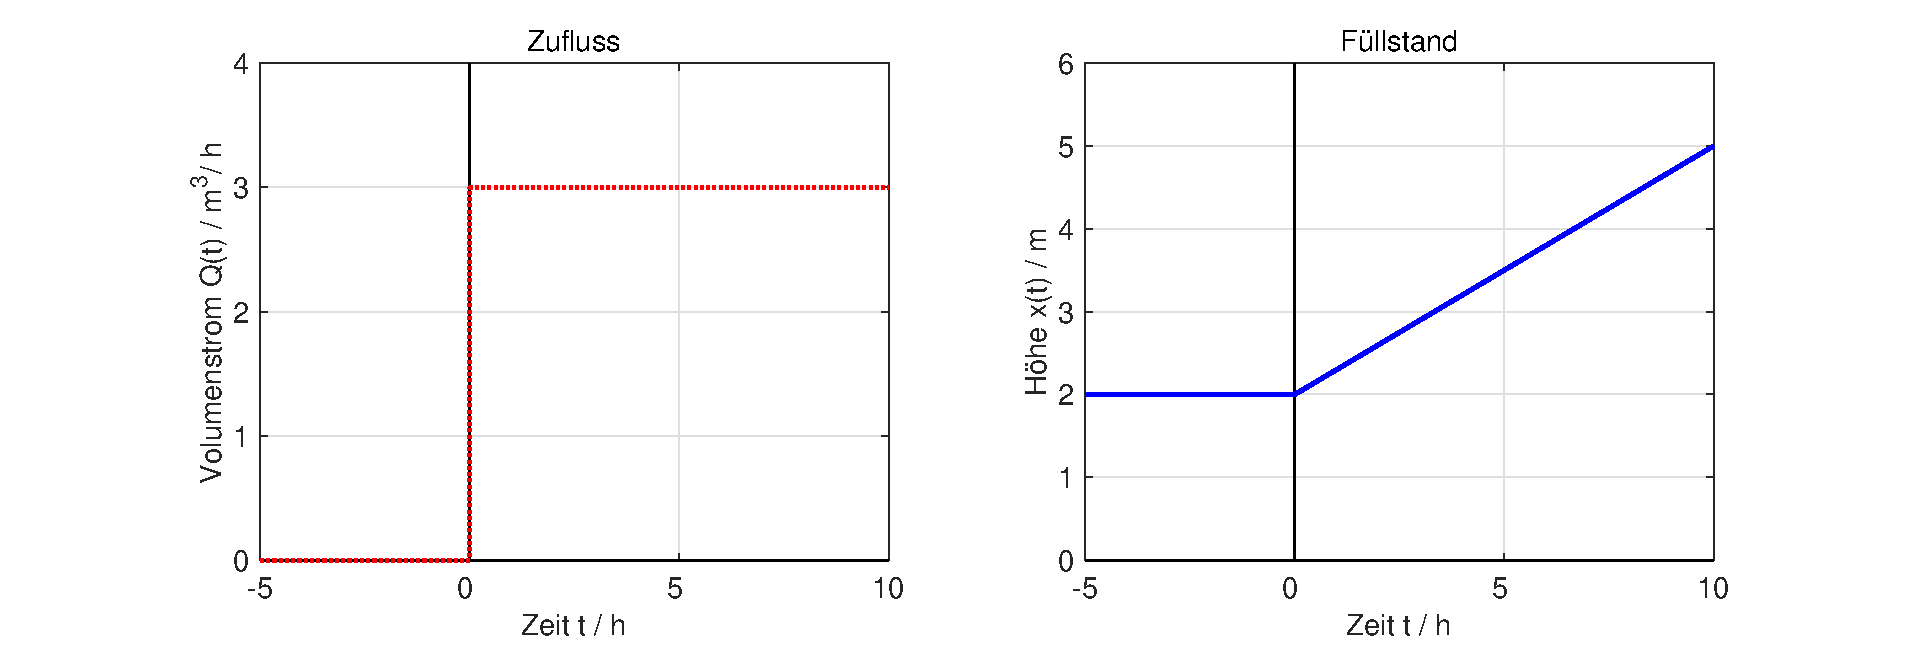
\includegraphics[width=0.3\textwidth]{Kapitel6/Bilder/image14}}
  \caption{Kapazitiver Feuchtesensor}
  \label{fig:Feuchtesensor}
\end{figure}

\noindent Der Sensor besteht aus einem Kondensator, der mit einem Dielektrikum gef\"{u}llt ist, das bei Aufnahme von Luftfeuchtigkeit seine Permittivit\"{a}tszahl $\epsilon_{R}$ \"{a}ndert. Es ergibt sich ein weitgehend linearer Zusammenhang zwischen Kapazit\"{a}t des Sensors und relativer Luftfeuchte. Die elektrische Auswertung f\"{u}hrt zu einem Sensorsignal, das vom Motorsteuerger\"{a}t erfasst wird.

\subsubsection{Hypothesentest als Diagnosefunktion f\"{u}r Feuchtesensoren}

\noindent Als M\"{o}glichkeit der Sensor\"{u}berwachung soll eine redundante Sensoranordnung bewertet werden. Dabei werden zwei identische Sensoren in das Modul integriert. Weichen beide Sensorsignale signifikant voneinander ab, ist zumindest einer der beiden Sensoren defekt.\newline

\noindent Zur mathematischen Beschreibung der Diagnoseaufgabe wird das Messergebnis des einen Sensors als x$_{1}$ und das Messergebnis des zweiten Sensors mit x$_{2}$ bezeichnet. F\"{u}r die Berechnung wird die Differenz des jeweiligen Messwertes x$_{n}$ zu seinem Sollverhalten $\mu_{n}$ bewertet. Unter diesen Bedingungen besitzt die Variable 

\begin{equation}\label{eq:sixonehundredsixty}
z=\dfrac{x_{1} -\mu _{1} -(x_{2} -\mu _{2})}{\sqrt{\sigma _{1}^{2} +\sigma _{2}^{2}}}
\end{equation}

\noindent eine Standardnormalverteilung. Die beiden Varianzen $\sigma_{1}^{2}$ und $\sigma_{2}^{2}$ sind gleich gro{\ss} und werden als $\sigma^{2}$ bezeichnet. Weiter wird davon ausgegangen, dass die aus der Erprobung der Sensoren bekannte Standardabweichung $\sigma$ typisch f\"{u}r den Einsatz der Sensoren im Kraftfahrzeug ist. Die Abweichungen der beiden Messwerte x$_{1}$ und x$_{2}$ sowie der beiden Mittelwerte $\mu_{1}$ und $\mu_{2}$ werden zusammengefasst, zu den Abweichungen $\Delta$x und $\Delta\mu$. Damit ergibt sich die standardnormalverteilte Variable

\begin{equation}\label{eq:sixonehundredsixtyone}
z=\dfrac{x_{1} -\mu _{1} -(x_{2} -\mu _{2})}{\sqrt{\sigma _{1}^{2} +\sigma _{2}^{2}}} =\dfrac{\Delta x-\Delta \mu }{\sqrt{2\cdot \sigma ^{2}}}
\end{equation}

\noindent Die Bewertung der Messergebnisse kann damit als Hypothesentest formuliert werden, bei dem gepr\"{u}ft wird, ob beide Sensoren voneinander abweichen.

\begin{itemize}
    \item Nullhypothese H$_{0}$: $\Delta$µ = 0
    \item Alternativhypothese H$_{1}$: $\Delta$µ $\neq$ 0
\end{itemize}

\noindent Unter der Annahme, dass die Nullhypothese richtig ist, ist $\Delta\mu$ = 0. Damit gilt unter dieser Annahme

\begin{equation}\label{eq:sixonehundredsixtytwo}
z=\dfrac{\Delta x}{\sqrt{2\cdot \sigma ^{2}}}
\end{equation}

\noindent Mit diesen Vor\"{u}berlegungen kann der Hypothesentest grafisch dargestellt werden.

\noindent 
\begin{figure}[H]
  \centerline{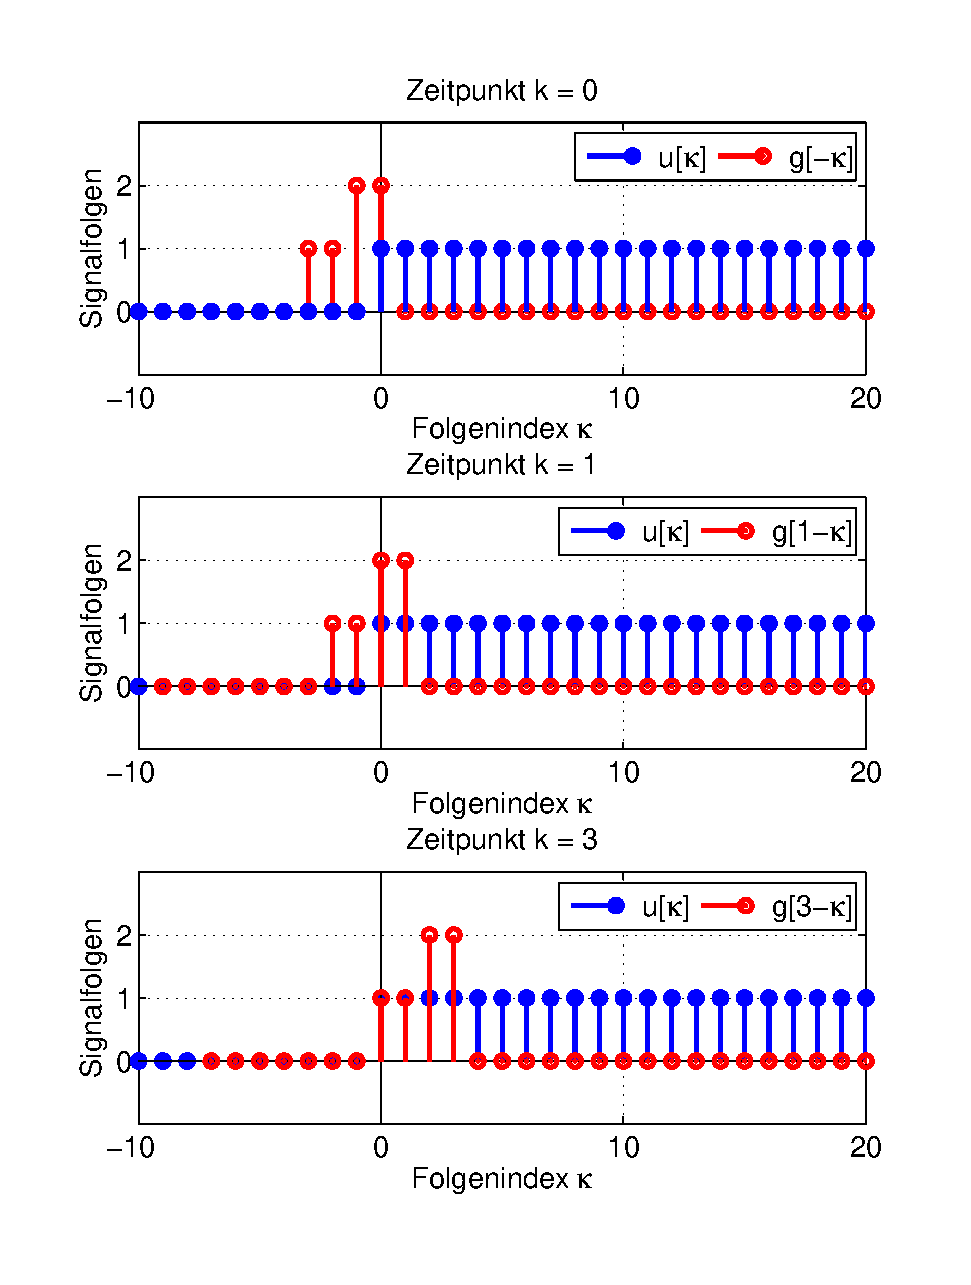
\includegraphics[width=0.5\textwidth]{Kapitel6/Bilder/image15}}
  \caption{Grafische Darstellung des Hypothesentests zur \"{U}berwachung zweier Feuchtesensoren}
  \label{fig:DiagnoseFeuchtesensor2}
\end{figure}

\noindent Damit eine \"{u}ber die Stichprobe gesch\"{a}tzte Abweichung $\Delta$x mit einer spezifizierten Wahrscheinlichkeit zu der Normalverteilung geh\"{o}rt, muss dieser in dem Intervall $\Delta$µ$_{C1} < \Delta$x $\leq$ $\Delta$µ$_{C2}$ liegen. Wird die Wahrscheinlichkeit daf\"{u}r mit $\gamma$ bezeichnet, gilt die Gleichung

\begin{equation}\label{eq:sixonehundredsixtythree}
P\left(\Delta \mu _{C1} <\Delta x\le \Delta \mu _{C2} \right)=\gamma
\end{equation}

\noindent Zur Berechnung der Grenzen $\Delta$µ$_{C1}$ und $\Delta$µ$_{C2}$ wird auf die standardnormalverteilte Zufallsvariable z zur\"{u}ckgegriffen. Mit der Definition der Zufallsvariable z in Gleichung \eqref{eq:sixonehundredsixtytwo} ist die Wahrscheinlichkeit $\gamma$, mit der die Variable z innerhalb des Intervalls c$_{1}$ {\dots} c$_{2}$ liegt, definiert als

\begin{equation}\label{eq:sixonehundredsixtyfour}
\gamma =P\left(c_{1} <z\le c_{2} \right)=F(c_{2})-F(c_{1})
\end{equation}

\noindent Da die Sensoren eine positive oder negative Drift aufweisen k\"{o}nnen, handelt es sich um einen symmetrischen Test. Damit ergeben sich die Konstanten c$_{1}$ und c$_{2}$ aus den Bedingungen

\begin{equation}\label{eq:sixonehundredsixtyfive}
F(c_{1})=\dfrac{1-\gamma}{2} =\dfrac{\alpha}{2}
\end{equation}

\noindent und

\begin{equation}\label{eq:sixonehundredsixtysix}
F(c_{2})=1-\dfrac{1-\gamma}{2} =1-\dfrac{\alpha}{2}
\end{equation}

\noindent Aufl\"{o}sen nach c$_{1}$ und c$_{2}$ f\"{u}hrt zu

\begin{equation}\label{eq:sixonehundredsixtyseven}
c_{1} =F^{-1} \left(\dfrac{\alpha}{2} \right)
\end{equation}

\noindent und

\begin{equation}\label{eq:sixonehundredsixtyeight}
c_{2} =F^{-1} \left(1-\dfrac{\alpha }{2} \right)
\end{equation}

\noindent Durch Umformungen von Gleichung \eqref{eq:sixonehundredsixtyfour} ergibt sich ein Ausdruck f\"{u}r den Annahmebereich der Nullhypothese

\begin{equation}\label{eq:sixonehundredsixtynine}
\gamma =P\left(c_{1} <\dfrac{\Delta x}{\sqrt{2\cdot \sigma ^{2} } } \le c_{2} \right)=P\left(c_{1} \cdot \sqrt{2\cdot \sigma ^{2} } <\Delta x\le c_{2} \cdot \sqrt{2\cdot \sigma ^{2} } \right)
\end{equation}

\noindent Zur numerischen Berechnung der Grenzwerte m\"{u}ssen die Konstanten c$_{1}$ und c$_{2}$ sowie die Varianz $\sigma^{2}$ bestimmt werden. Aus Kapitel 2 ist bekannt, dass die Wahrscheinlichkeit, mit der ein funktionst\"{u}chtiger Sensor als defekt eingestuft wird, klein gehalten werden muss. Deshalb wird ein Signifikanzniveau von $\alpha$ = 10 ppm gew\"{a}hlt. Daraus ergeben sich die Grenzen

\begin{equation}\label{eq:sixonehundredseventy}
c_{1} =F^{-1} \left(\dfrac{\alpha }{2} \right)=-4.4172
\end{equation}

\noindent und

\begin{equation}\label{eq:sixonehundredseventyone}
c_{2} =F^{-1} \left(1-\dfrac{\alpha }{2} \right)=4.4172
\end{equation}

\noindent Im Rahmen von Freigabeerprobungen wurden Sensoren unterschiedlichen Tests unterzogen. Bei diesen Tests wurden funktionsf\"{a}hige Sensoren im laufenden Betrieb bewertet. Eine Zusammenfassung der Messergebnisse zeigt Bild \ref{fig:DiagnoseFeuchtesensor3}.

\noindent 
\begin{figure}[H]
  \centerline{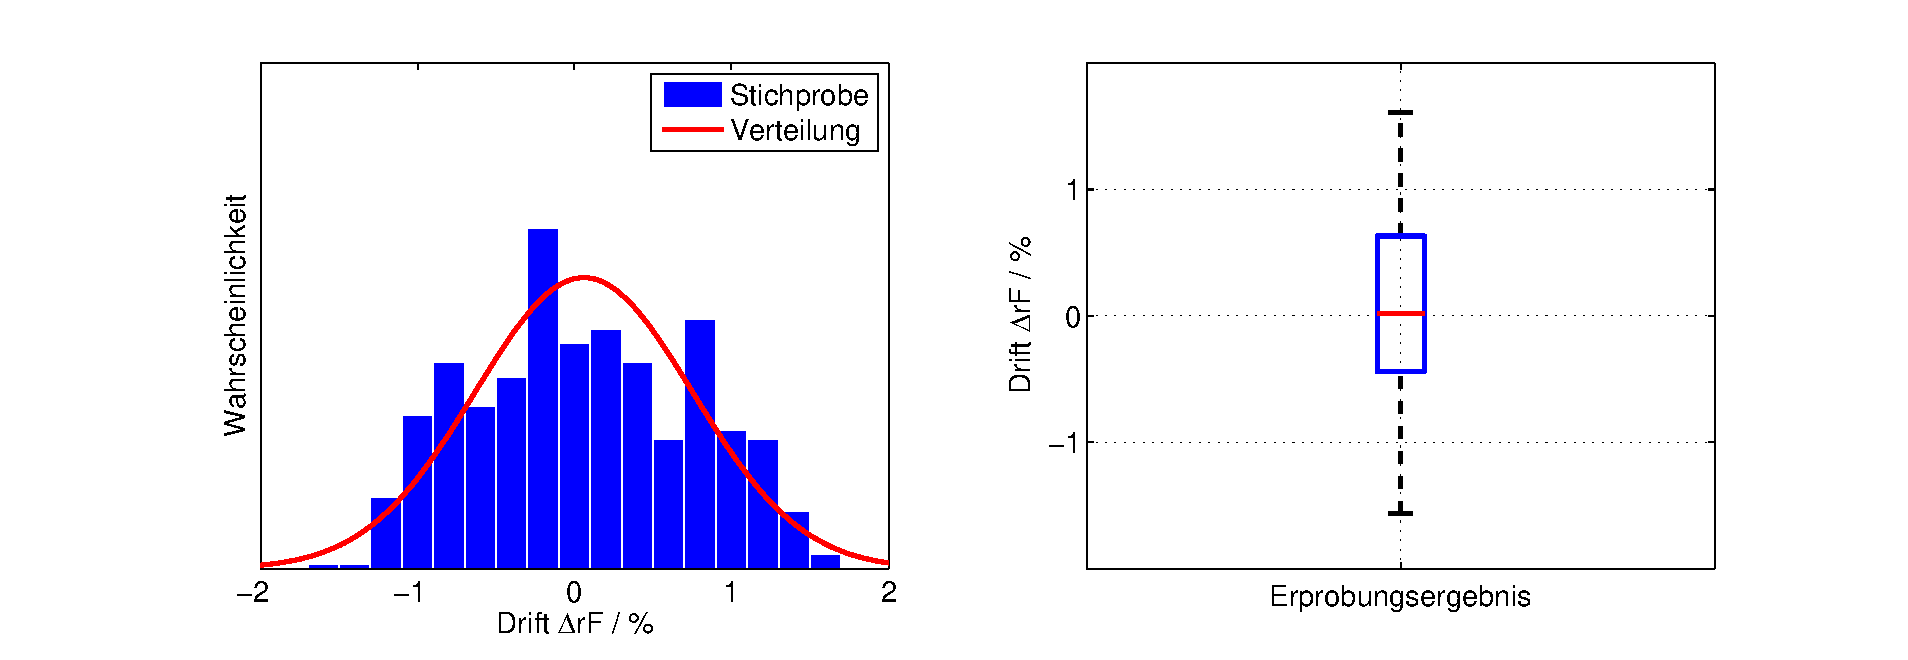
\includegraphics[width=1\textwidth]{Kapitel6/Bilder/image16}}
  \caption{Statistische Zusammenfassung aller Driften bei einer Freigabeerprobung}
  \label{fig:DiagnoseFeuchtesensor3}
\end{figure}

\noindent Die Stichprobe weist eine Standardabweichung von s = 0.6931 \% auf. Die Messergebnisse werden als repr\"{a}sentativ f\"{u}r Driften im Fahrzeugbetrieb angenommen. Es wird deshalb von einer Standardabweichung der Grundgesamtheit von $\sigma$ = 0.6931 \% ausgegangen. Daraus ergeben sich f\"{u}r die Annahme der Hypothese die Grenzen

\begin{equation}\label{eq:sixonehundredseventytwo}
-4.4172\cdot \sqrt{2} \cdot 0.6931 <\Delta x\le 4.4172\cdot \sqrt{2} \cdot 0.6931
\end{equation}

\noindent beziehungsweise

\begin{equation}\label{eq:sixonehundredseventythree}
- 4.3298 \% <\Delta x\le 4.3298 \%
\end{equation}

\noindent Liegt die Abweichung $\Delta$x bei einer Feuchte von rF = 85 \% au{\ss}erhalb dieser Grenzen, ist der Sensor als defekt einzustufen.

\subsubsection{G\"{u}te der Diagnosefunktion f\"{u}r Feuchtesensoren}

\noindent Die Diagnosegrenzen werden unter Annahme der Nullhypothese $\Delta\mu$ = 0 mit dem Fehler erster Art festgelegt. Im Betrieb der Diagnosefunktion bleiben die Diagnosegrenzen fest. Liegt der Stichprobenwert in den Grenzen

\begin{equation}\label{eq:sixonehundredseventyfour}
-  4.3298 \% <\Delta x\le  4.3298 \%
\end{equation}

\noindent wird der Sensor als funktionsf\"{a}hig eingestuft. Der Sensor wird als defekt eingestuft, wenn ein Stichprobenwert $\Delta$x unterhalb der Grenze $\Delta$x $\leq$ - 4.3298 oder oberhalb der Grenze $\Delta$x $ > $ 4.3298 liegt. Da der Stichprobenwert $\Delta$x von der wahren Differenz der Sensordriften $\Delta\mu$ abh\"{a}ngt, ist auch die Wahrscheinlichkeit der Einstufung des Sensors als defekter Sensor eine Funktion der Gr\"{o}{\ss}e $\Delta\mu$. Sie ist definiert als 

\begin{equation}\label{eq:sixonehundredseventyfive}
1-\beta \left(\Delta \mu \right)=1-P\left(c_{1} <\dfrac{\Delta x-\Delta \mu }{\sqrt{2\cdot \sigma ^{2} } } \le c_{2} \right)
\end{equation}

\noindent Da die Variable z mit den dargestellten Annahmen standardnormalverteilt ist, kann die G\"{u}te mit den bekannten Grenzen c$_{1}$ und c$_{2}$ sowie der Standardabweichung $\sigma$ = 0.6931 \% berechnet werden aus 

\begin{equation}\label{eq:sixonehundredseventysix}
\begin{split}
1-\beta \left(\Delta \mu \right) & = 1-F\left(\dfrac{\Delta \mu _{C1} -\Delta \mu }{\sqrt{2\cdot \sigma ^{2}}} \right)+F\left(\dfrac{\Delta \mu _{C2} -\Delta \mu }{\sqrt{2\cdot \sigma ^{2}}} \right) \\ 
& = 1-F\left(\dfrac{-4.3298 \% -\Delta \mu }{0.9802} \right)+F\left(\dfrac{4.3298 \% -\Delta \mu }{0.9802} \right)   
\end{split}
\end{equation}

Bild \ref{fig:DiagnoseFeuchtesensor4} stellt die G\"{u}te des Hypothesentests mit der Alternativhypothese $\Delta$µ $\neq$ 0 als Funktion des alternativen Mittelwertes $\Delta$µ dar. 

\noindent 
\begin{figure}[H]
  \centerline{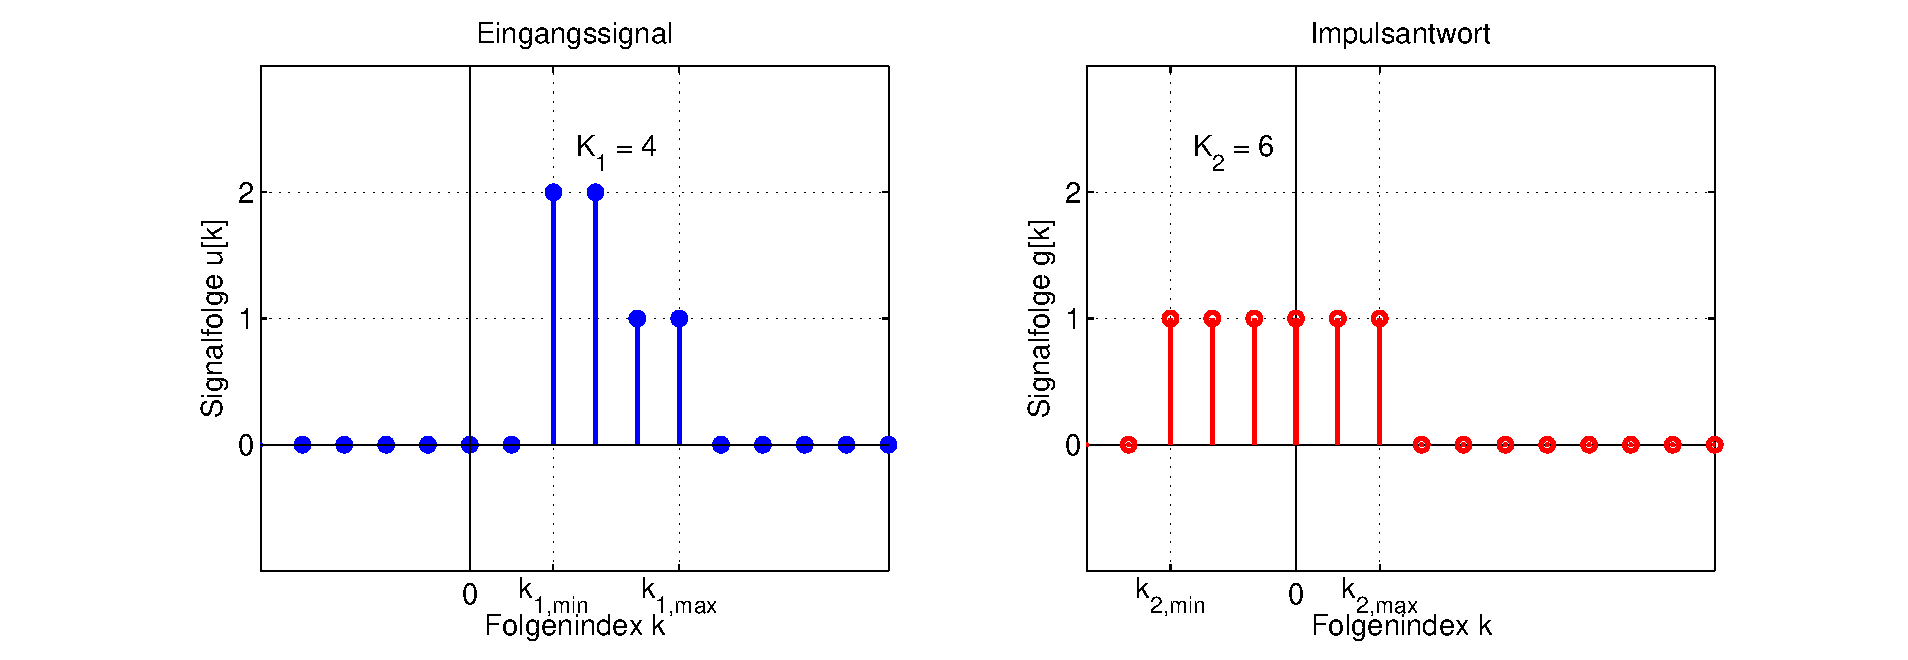
\includegraphics[width=0.5\textwidth]{Kapitel6/Bilder/image17}}
  \caption{Darstellung der G\"{u}tefunktion f\"{u}r die Alternative $\Delta$µ $\neq$ 0}
  \label{fig:DiagnoseFeuchtesensor4}
\end{figure}

\noindent Mit steigendem Abstand $\Delta\mu$ von dem Wert $\Delta\mu$ = 0 steigt die Wahrscheinlichkeit f\"{u}r die Einstufung als defekten Sensor. Eine Sensordrift von $\Delta\mu$ = - 5 \% wird mit einer Wahrscheinlichkeit von 75.2 \% richtig diagnostiziert.

\clearpage

\subsection{Literatur}

\begin{tabular}{|p{0.6in}|p{5.6in}|} \hline 
[Krey91] & Kreyszig, Erwin: Statistische Methoden und ihre Anwendungen\newline 4., unver\"{a}nderter Nachdruck der 7. Auflage\newline Vandenhoeck \& Ruprecht, G\"{o}ttingen, 1991 \\ \hline 
[Fahr06] & Fahrmeir, Ludwig; K\"{u}nstler, Rita; Pigeot, Iris; Tutz, Gerhard: Der Weg zur Datenanalyse\newline 6. Auflage\newline Springer Berlin Heidelberg New York, 2006 \\ \hline 
[Ross06] & Ross, M. Sheldon: Statistik f\"{u}r Ingenieure und Naturwissenschaftler\newline 3. Auflage\newline Spektrum Akademischer Verlag, M\"{u}nchen, 2006 \\ \hline 
[Papu01] & Papula, Lothar: Mathematik f\"{u}r Ingenieure und Naturwissenschaftler Band 3\newline 4., verbesserte Auflage\newline Vieweg Teubner, Braunschweig / Wiesbaden, 2008 \\ \hline 
\end{tabular}
